\section{Results}
\label{sec:DiHiggs:results}

The set up used for the profile likelihood fit is described in section~\ref{sec:DiHiggs:analysis}.
In section~\ref{sec:DiHiggs:lephadonly}, results obtained from 
\lephad only fit (using only the \lephad signal regions and the \ZHF\ control region)
are presented.
The result from the likelihood fit shows that the data is compatible with
the null hypothesis for all signals. Therefore, the data is used to set
upper limits at 95\% C.L.\ on the signal cross-sections. 
The likelihood fit is performed again on the \lephad and 
\hadhad signal regions and the \ZHF\ control region,
and the results are presented in
section~\ref{sec:DiHiggs:combination-bbtautau}.
The fit results in \bbtt channel are then combined with the \bbyy channel
for upper limits on the non-resonant SM $HH$ production cross-section and 
limits on the self-coupling modifier \kl,
and with the \bbyy, \bbbb channels for upper limits
on the narrow-width scalar $X$ production cross-section as a function of resonance mass.
These combinations results are presented in section~\ref{sec:DiHiggs:combination-HH}.

\subsection{Fit setup}
\label{sec:DiHiggs:analysis}

The profile likelihood fit is first performed on the MVA output in the \lephad SLT, LTT regions, 
together with the $m_{ll}$ distribution in the 
\ZHF\ control region, referred to as \lephad only fit. After checking the \lephad only fit results, 
a likelihood fit is then performed simultaneously on the MVA output in all three signal regions, the \lephad SLT, LTT
and the \hadhad regions, together with the $m_{ll}$ distribution in the \ZHF\ control region.
As described in Section~\ref{sec:DiHiggs:MVA}, for the resonant $HH$ production, PNNs are used for 
signal extraction, and for the non-resonant production, a neural network is used in the \lephad channel 
(a Boosted Decision Tree, BDT is used for the non-resonant production in the \hadhad signal region).  
% For each tested signal hypothesis a binned profile likelihood ratio fit is performed on the MVA output distributions.

The normalisation of the $t\bar{t}$ background and the normalisation of the \ZHF\ background 
are determined in the fit as freely floating parameter.  
Relative acceptance uncertainties between CR and SRs are applied on 
these normalisations in the signal regions included in the fit as described in Section~\ref{sec:DiHiggs:systematics}.

The Parameter Of Interest (POI) is the signal strength $\mu$.  
As described in section TODO: ref the theory section For the non-resonant SM case, the $\mu$ is relative to the ggF+VBF input signal cross-section 
of (31.05 + 1.726 ) fb$\times \text{BR}_{HH\rightarrow bb\tau\tau}$ =  32.776 fb$\times \text{BR}_{HH\rightarrow bb\tau\tau}$,
% Fits considering only ggF signal and neglecting VBF are also performed as a cross check where the $\mu$ is relative to the ggF input signal cross-section of 31.05 x BR. 
and for the resonant case,  the $\mu$  is relative to the input cross-section of 1 pb$\times \text{BR}_{HH\rightarrow bb\tau\tau}$.

In the \lephad channel, the MVA outputs are binned in 1090 bins, where 990 bins with equal width are in the range from 0 to 0.99 
and 100 bins with equal width are in the range from 0.99 to 1.
A rebinning procedure is performed on the MVA output. 
First, a rebinning metric is defined as:
\begin{equation}
Z(I[k,l]) = 10 \frac{n_{s}(I[k,l])}{N_{s}} + 5 \frac{n_{b}(I[k,l])}{N_{b}},
\end{equation}
where
\begin{itemize}
\item $I[k,l]$ is an interval of the histograms, containing the bins between bin $k$ and bin $l$;
\item $N_{s}$ is the total number of signal events in the histogram;
\item $N_{b}$ is the total number of background events in the histogram;
\item $n_{s}(I[k,l])$ is the total number of signal events in the interval $I[k,l]$;
\item $n_{b}(I[k,l])$ is the total number of background events in the interval $I[k,l]$.
\end{itemize}
The re-binning is then conducted using the following procedure:
\begin{enumerate}
\item Starting from the first bin $k_0$ on the right end of the MVA output histogram (MVA output = 1), 
increase the range of the interval $I(k_0, l)$ 
by adding one after the other to the left;
\item Calculate the value of Z at each step;
\item Once $Z(I[k_{0}, l]) > 1$, rebin all the bins in the interval $I(k_{0}, l)$ into a single bin;
\item Repeat steps 1-3, starting this time from the last bin on the right (bin $l+1$, the next bin to the left of bin $l$)
until reaches the left end (0) of the histogram.
\end{enumerate}
In addition, binning algorithm requires at least 5 background events in each bin. 

All sources of systematic uncertainties described in Section~\ref{sec:DiHiggs:systematics} 
are considered as nuisance parameters
in the profile likelihood. 
Correlations of NPs across the four regions are included in the fit.
All experimental uncertainties,
modelling uncertainties from the same source 
(except for the fake background which was estimated using different
method in the \lephad and \hadhad channel ),
\ttbar\ and \ZHF\ background normalisations and 
relative acceptance uncertainties on \ttbar\ and \ZHF\ backgrounds
are correlated across the three signal regions and one control region. 


Each NP is split into shape and normalisation effects. 
The shape uncertainties are included as alternative histograms while the
normalisation effects are implemented as either flat (for the floating backgrounds)
or Gaussian priors. 
The NPs are then processed to be symmetrised, smoothed and pruned:
for one-sided experimental systematics and systematics with up and 
down variation going to the same side, symmetrisation is applied to 
avoid under-constraint problems and to improve the stability of fitting;
and then, smoothing is applied on systematics with large 
statistical fluctuations to avoid instabilities;
finally, systematics which have less impact are pruned away to speed up
the fitting process.






\subsection{\lephad channel results}
\label{sec:DiHiggs:lephadonly}
The profile likelihood fit is first performed on the two signal regions 
in the \lephad and the \ZHF\ control region. 
This section describes the fit reults obtained with this setting. 

\subsubsection{Post-fit background events yields}

The expected signal and background events yields  
passing the signal region event pre-selection after the \lephad only fit 
are shown in Table~\ref{tab:LepHadSLTPostfitYields} 
(\ref{tab:LepHadLTTPostfitYields}) for the SLT (LTT) channel, extacted from the 
fit result using NN output SM $HH$ as input. 



\begin{table}[htbp]
\centering
\begin{tabular}{|c|c|c|}
    \hline
\hline
SampleName &  Integral & Error \\
\hline
\multicolumn{3}{|c|}{\textbf{Signal Samples}} \\
\hline
ggF+VBF Non-resonant   & 6& 1   \\ 
\hline
\multicolumn{3}{|c|}{\textbf{Background Samples}} \\
\hline
Fake & 33100 & 1600\\
\ttbar & 58500 & 1500\\
single top & 3730 & 480\\
Ztthf & 1640 & 140\\
Zhf & 921 & 83\\
Zttlf & 80 & 22\\
Zlf & 57 & 19\\
SM Higgs & 153 & 19\\
diboson & 150 & 36\\
W & 73 & 30\\
Wtt & 5 & 2.2\\
DYtt & 1.7 & 1.9\\
DY & 12.8 & 3.7\\
\hline
total Bkg & 98450 & 680\\
\hline
data & 98456 & \\
\hline
%   Signal & 6 $\pm$ 1\\
%   SignalExpected & 6 $\pm$ 1\\
\end{tabular}
\caption{Post-fit event yields in the SLT signal region for the data, 
background and signal. Background names conventions are the same as used in 
Table~\ref{tab:LepHadSLTYields}.}
\label{tab:LepHadSLTPostfitYields}
\end{table}

\begin{table}[htbp]
\centering
\begin{tabular}{|c|c|c|}
\hline
\hline
SampleName &  Integral & Error \\
\hline
\multicolumn{3}{|c|}{\textbf{Signal Samples}} \\
\hline
ggF+VBF Non-resonant   & 1.44&0.24    \\ 
\hline
\multicolumn{3}{|c|}{\textbf{Background Samples}} \\
\hline
Fake & 1540 & 180\\
\ttbar & 3940 & 190\\
single top & 203 & 40\\
Ztthf & 537 & 65\\
Zhf & 52.6 & 7.1\\
Zttlf & 42 & 12\\
Zlf & 2.1 & 1.1\\
SM Higgs & 24 & 4.8\\
diboson & 19.9 & 4.6\\
W & 1.27 & 0.6\\
Wtt & 2.6 & 1.1\\
DYtt & 0.27 & 0.13\\
DY & 0.62 & 0.28\\
\hline
total Bkg & 6359 & 80\\
\hline
data & 6351 & \\ 
\hline
% \hline
% Signal & 1.44 $\pm$ 0.24\\
% SignalExpected & 1.44 $\pm$ 0.24\\

\end{tabular}
\caption{Post-fit event yields in the LTT signal region for the data, 
background and signal. Background names conventions are the same as used in 
Table~\ref{tab:LepHadLTTYields}.}
\label{tab:LepHadLTTPostfitYields}
\end{table}

The determined floating normalisations of the \ttbar\ and \ZHF\ background
are shown in Table~\ref{tab:LepHadNormfactor}.
The normalisation factors depend on which MVA output is used  
as input for the fit, as a result of different binnings which 
were optimised for different MVA output.


\begin{table}[htbp]
\centering
\begin{tabular}{|c|c|c|}
\hline
Mass point & \ZHF\ norm. factor & \ttbar\ norm. factor \\  
\hline
SM & 1.38 $\pm$ 0.11 &  0.96 $\pm$ 0.03 \\
300 GeV & 1.38 $\pm$ 0.11 &  0.97 $\pm$ 0.04 \\
500 GeV & 1.37 $\pm$ 0.11 &  0.97 $\pm$ 0.04 \\
1000 GeV & 1.39 $\pm$ 0.11 &  0.97 $\pm$ 0.04 \\
1600 GeV & 1.37 $\pm$ 0.11 &  0.97 $\pm$ 0.04 \\
\hline
\end{tabular}
\caption{Post-fit normalisation factors of \ttbar\ and \ZHF\ background obtained from the \lephad only fit 
for SM $HH$, 300, 500, 1000 and 1600 GeV resonance fit.}
\label{tab:LepHadNormfactor}
\end{table}



\subsubsection{Post-fit MVA input and output distributions}

The post fit MVA input variables distributions are shown in Figure~\ref{fig:sltmvainputspostfit} 
(\ref{fig:lttmvainputspostfit})
for the SLT (LTT) channel.
The post-fit PNN score distributions for the 300, 
500, 1000, 1600 GeV resonant mass points and 
the post-fit SM NN distribution in the SLT and LTT
channel are shown in Figure~\ref{fig:LepHadPostfitPNNScoreDistributions}.
As compared to the pre-fit MVA input and output distributions presented in section~\ref{sec:DiHiggs:MVA}, 
the post-fit distributions show much better MC and data agreement. 
The uncertainties are also more constrained with the help of the \ZHF\ control region. 

To validate the background modelling, the post-fit NN/PNNs distributions are 
checked in the 1-$b$-tag where the same signal region selection is applied except for
requiring exactly one \bjet. The background distributions are plotted against the data, as 
shown in Figure~\ref{fig:lephadmvaCRoutputpostfit} in Appendix~\ref{sec:appendix:result}.
In this validation region, the data is well modelled by the MC simulation within uncertainties.


\begin{figure}[htbp]
\centering
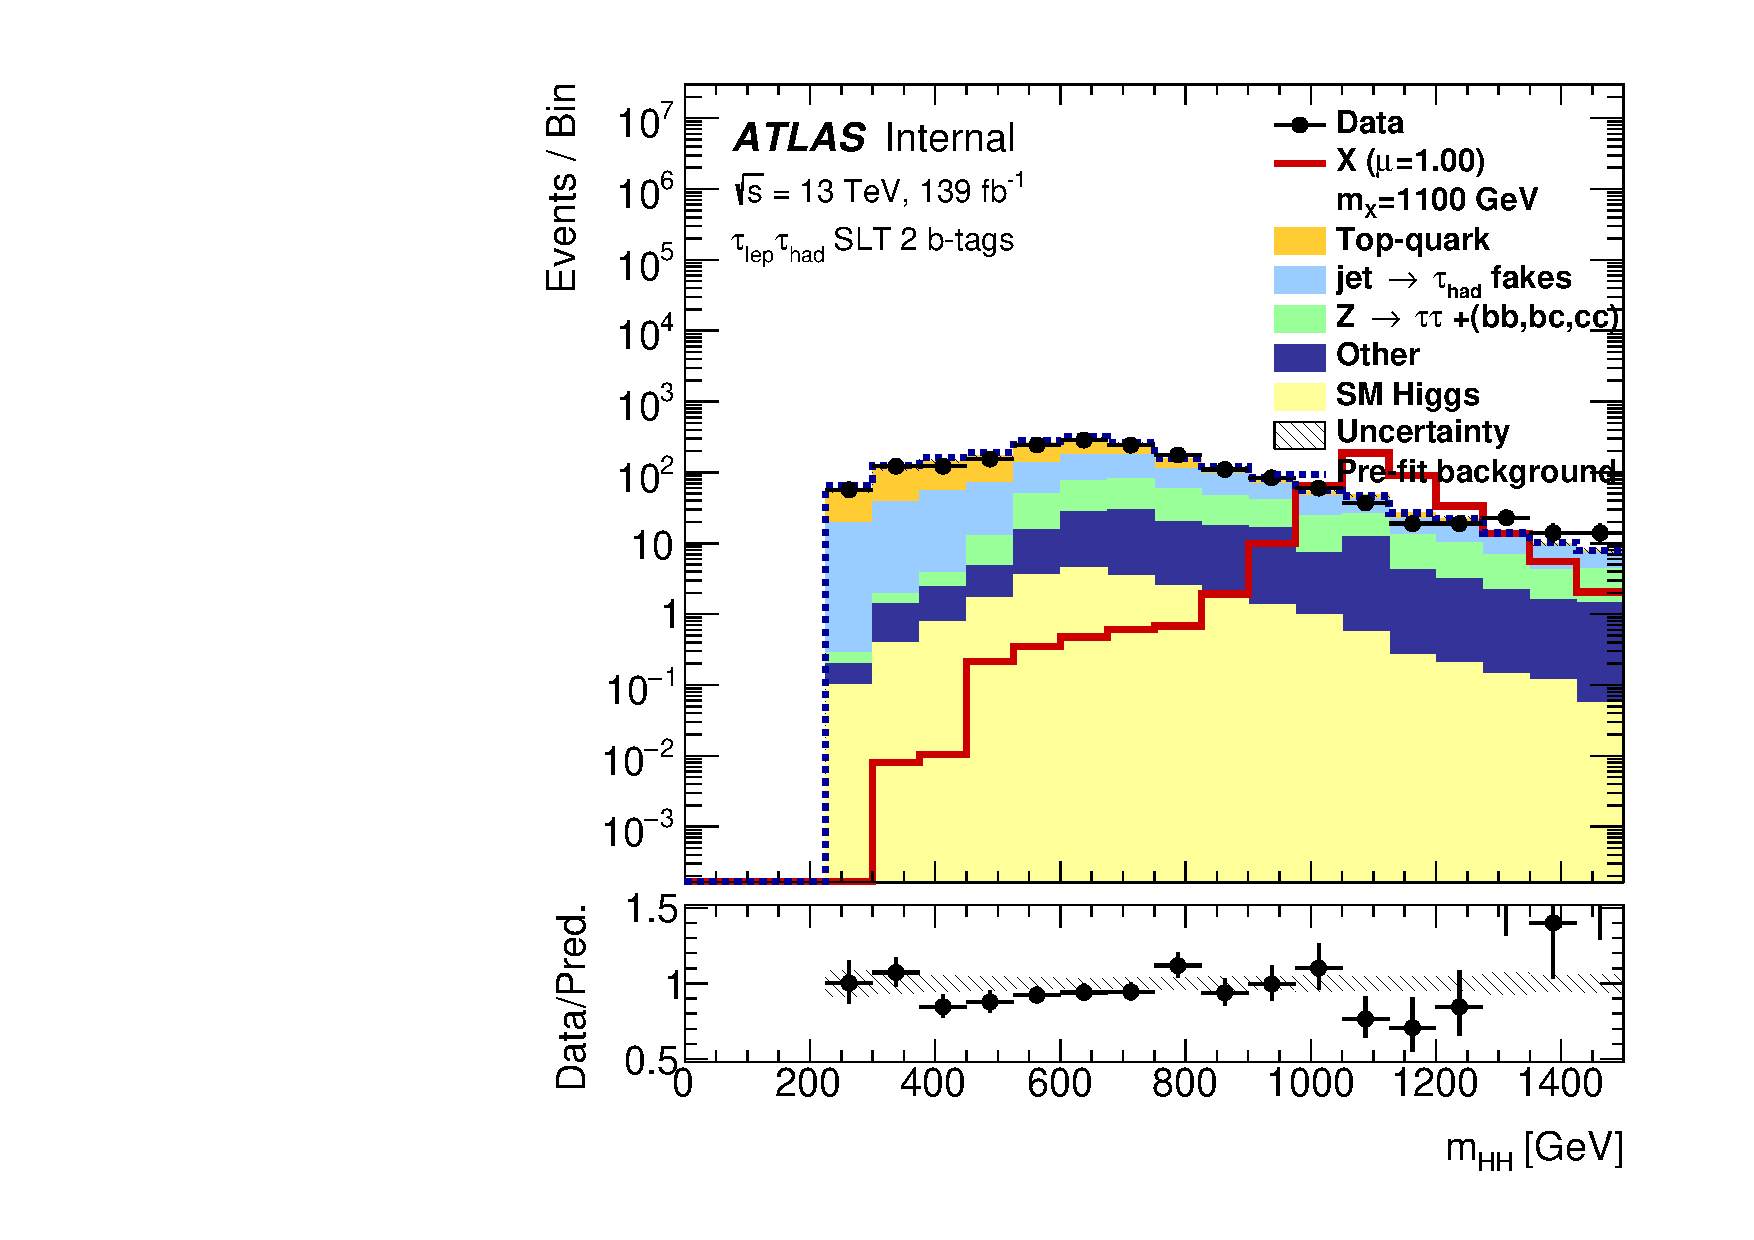
\includegraphics[width=.32\textwidth]{diHiggs/plots/MVA/postfit/Region_BMin0_incJet1_distMhh_J2_D_T2_SpcTauLH_Y2015_LTT0_L1_GlobalFit_conditionnal_mu0log.pdf}
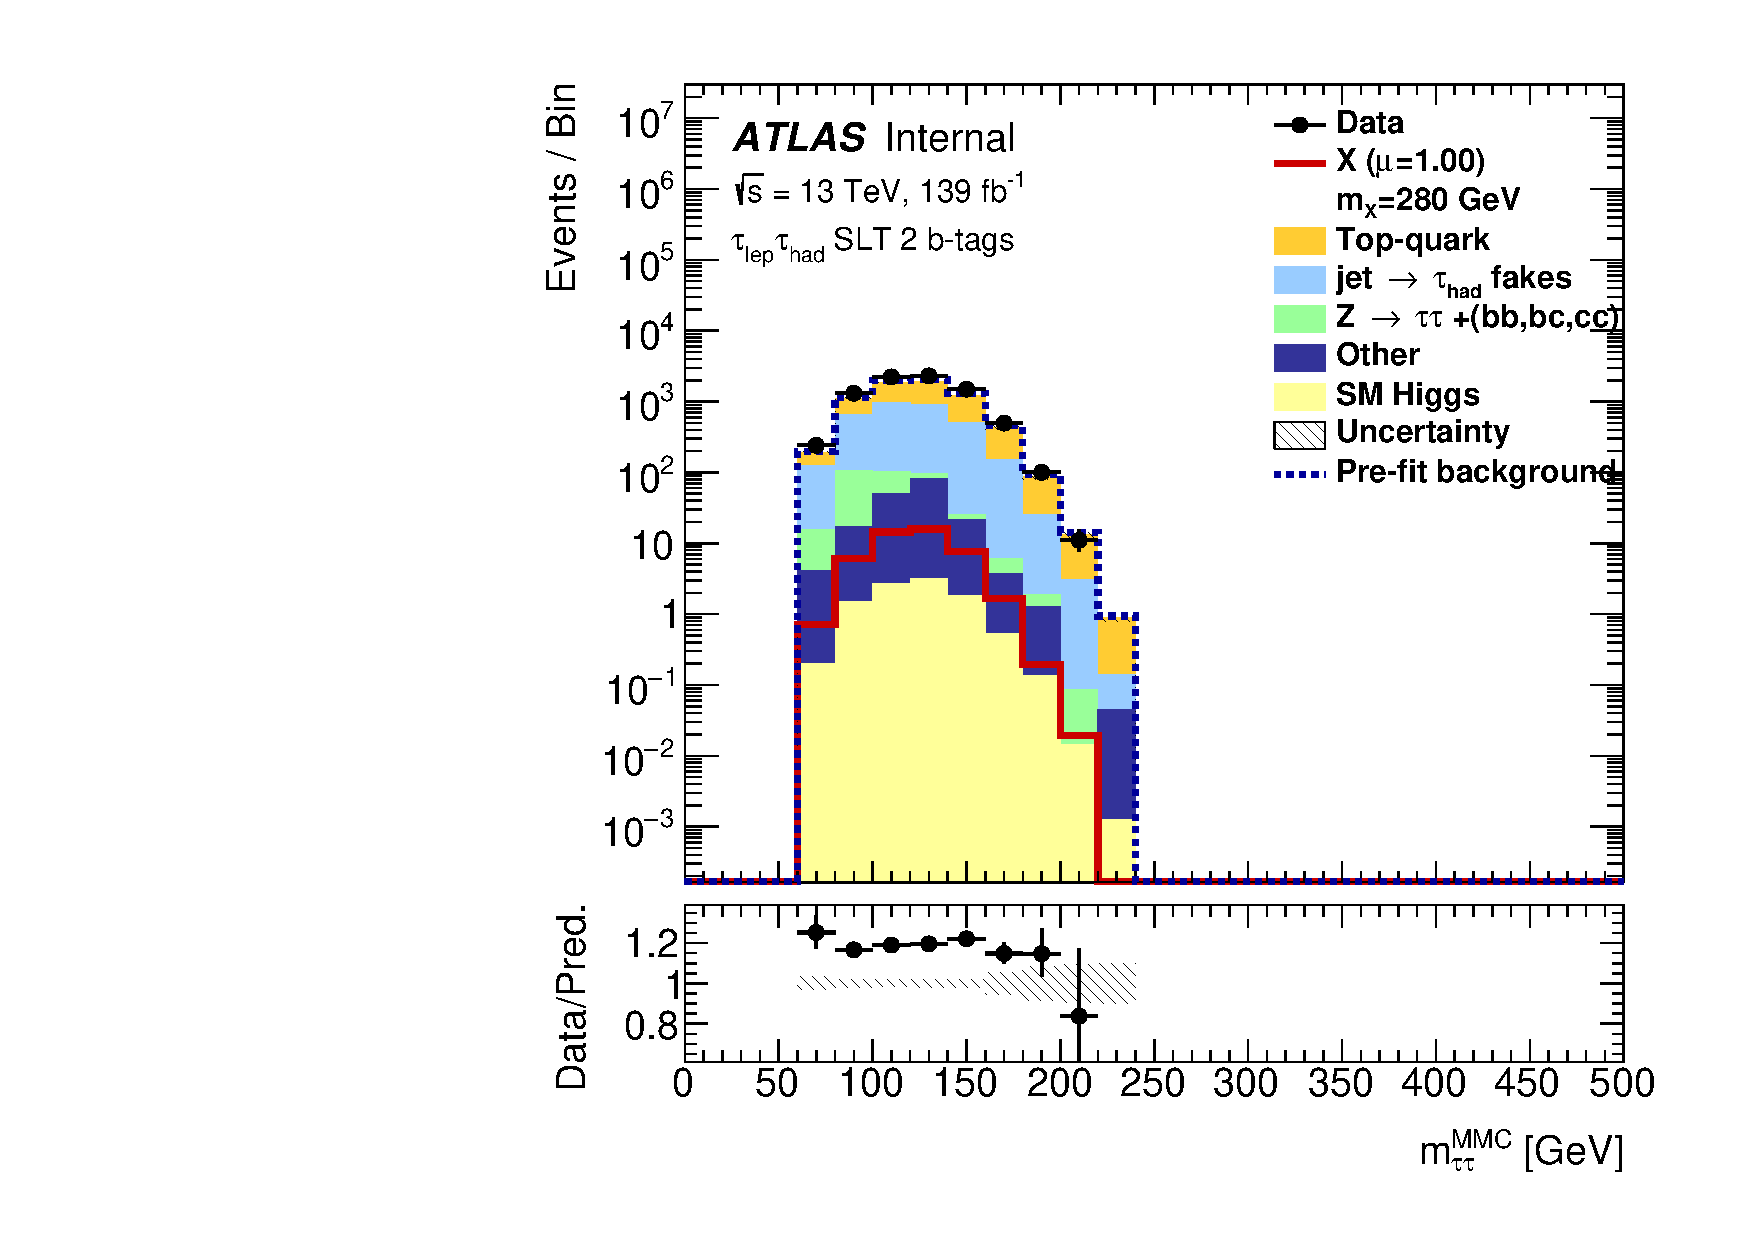
\includegraphics[width=.32\textwidth]{diHiggs/plots/MVA/postfit/Region_BMin0_incJet1_distmMMC_J2_D_T2_SpcTauLH_Y2015_LTT0_L1_GlobalFit_conditionnal_mu0log.pdf}
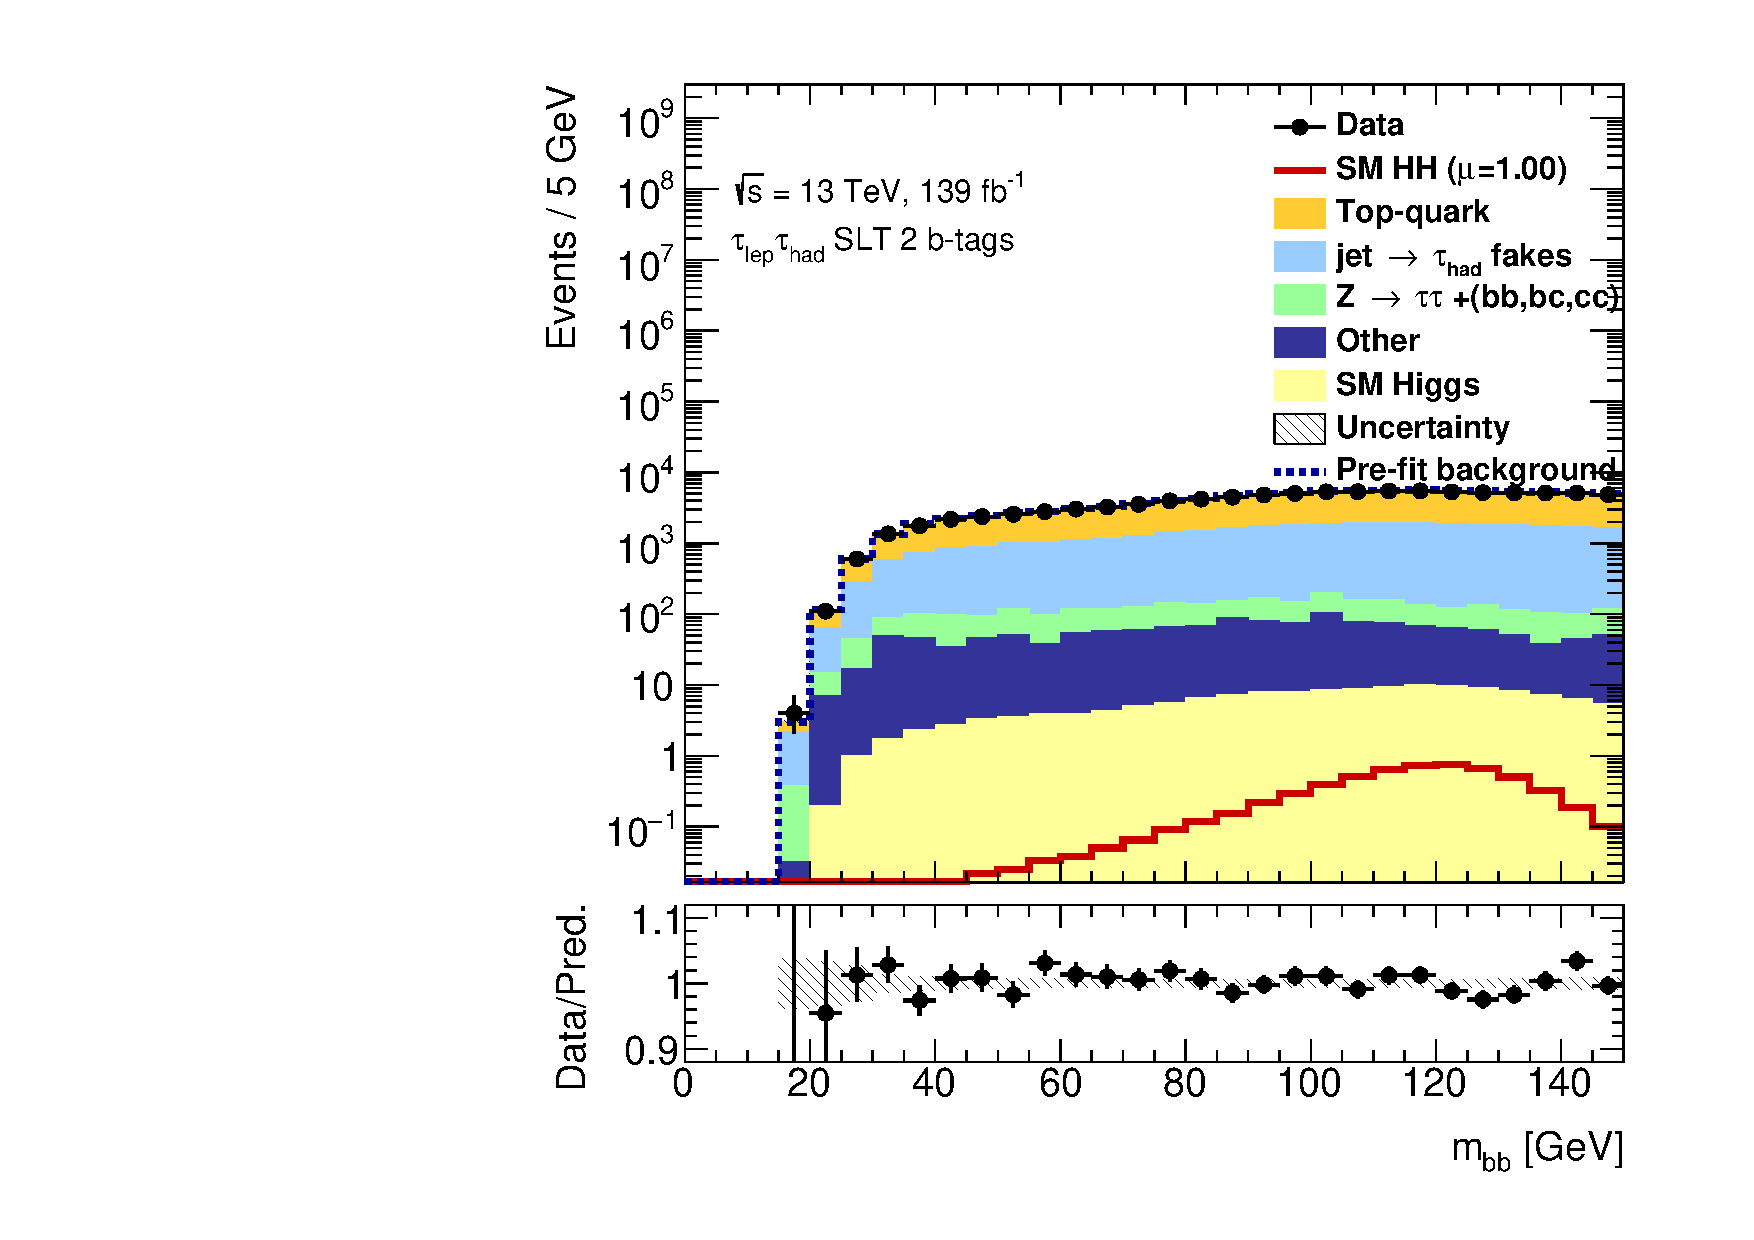
\includegraphics[width=.32\textwidth]{diHiggs/plots/MVA/postfit/Region_BMin0_incJet1_distmbb_J2_D_T2_SpcTauLH_Y2015_LTT0_L1_GlobalFit_conditionnal_mu0log.pdf} \\
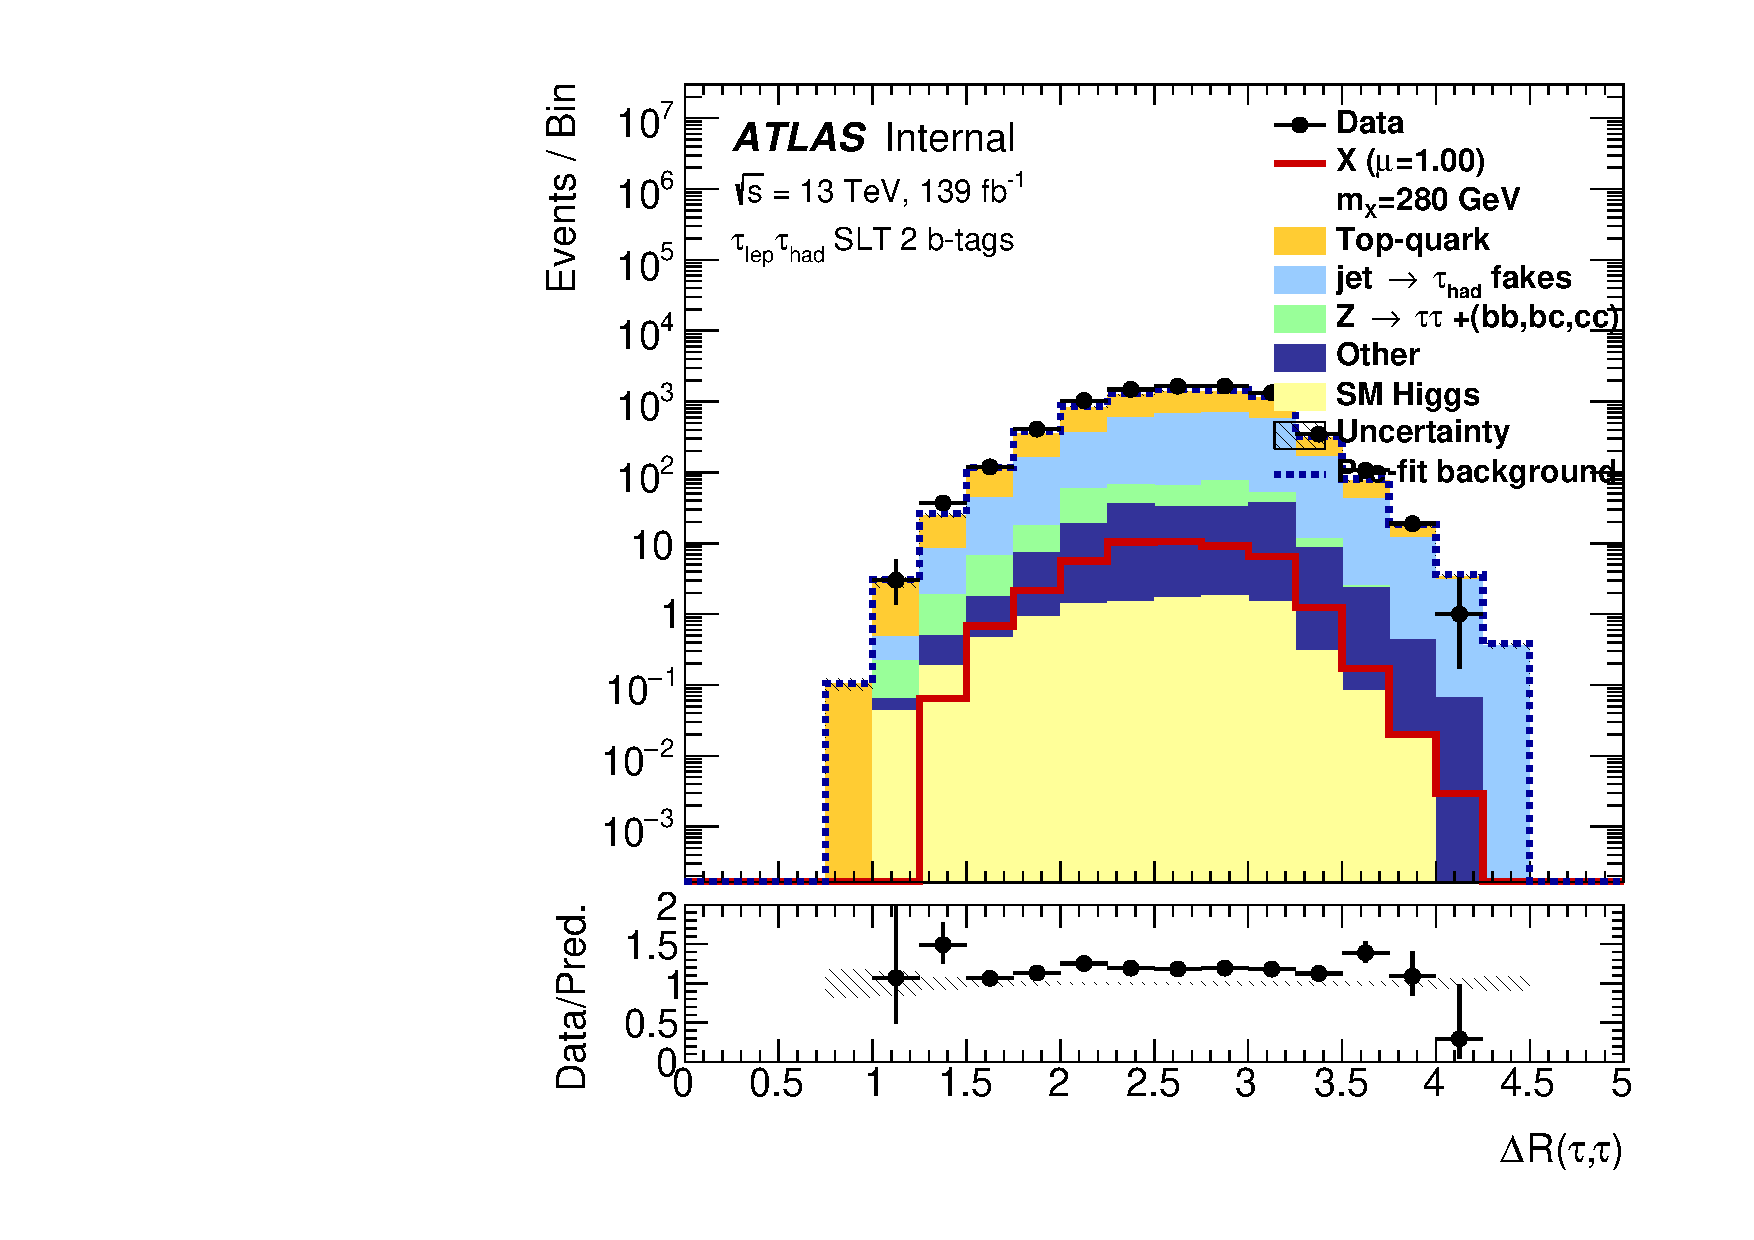
\includegraphics[width=.32\textwidth]{diHiggs/plots/MVA/postfit/Region_BMin0_incJet1_distDRTauTau_J2_D_T2_SpcTauLH_Y2015_LTT0_L1_GlobalFit_conditionnal_mu0log.pdf}
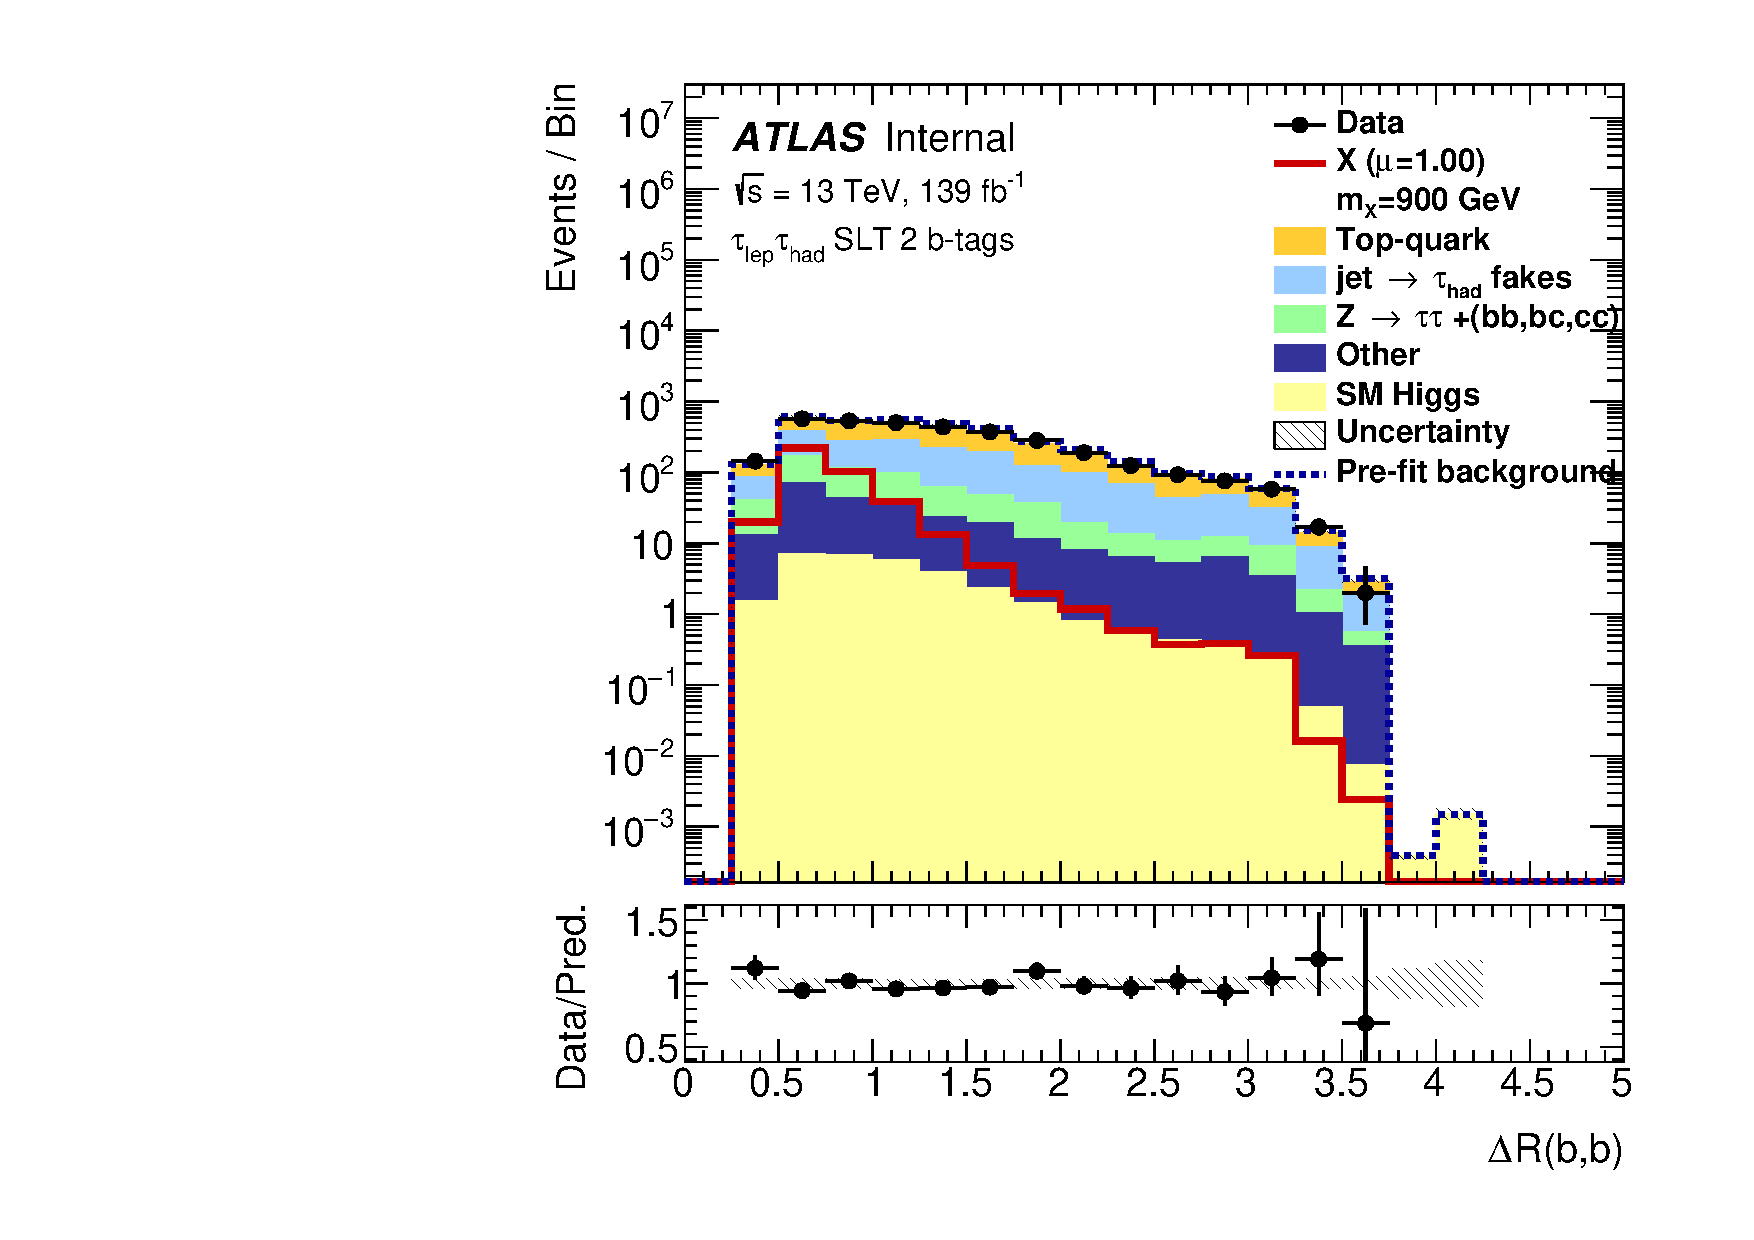
\includegraphics[width=.32\textwidth]{diHiggs/plots/MVA/postfit/Region_BMin0_incJet1_distdRbb_J2_D_T2_SpcTauLH_Y2015_LTT0_L1_GlobalFit_conditionnal_mu0log.pdf}
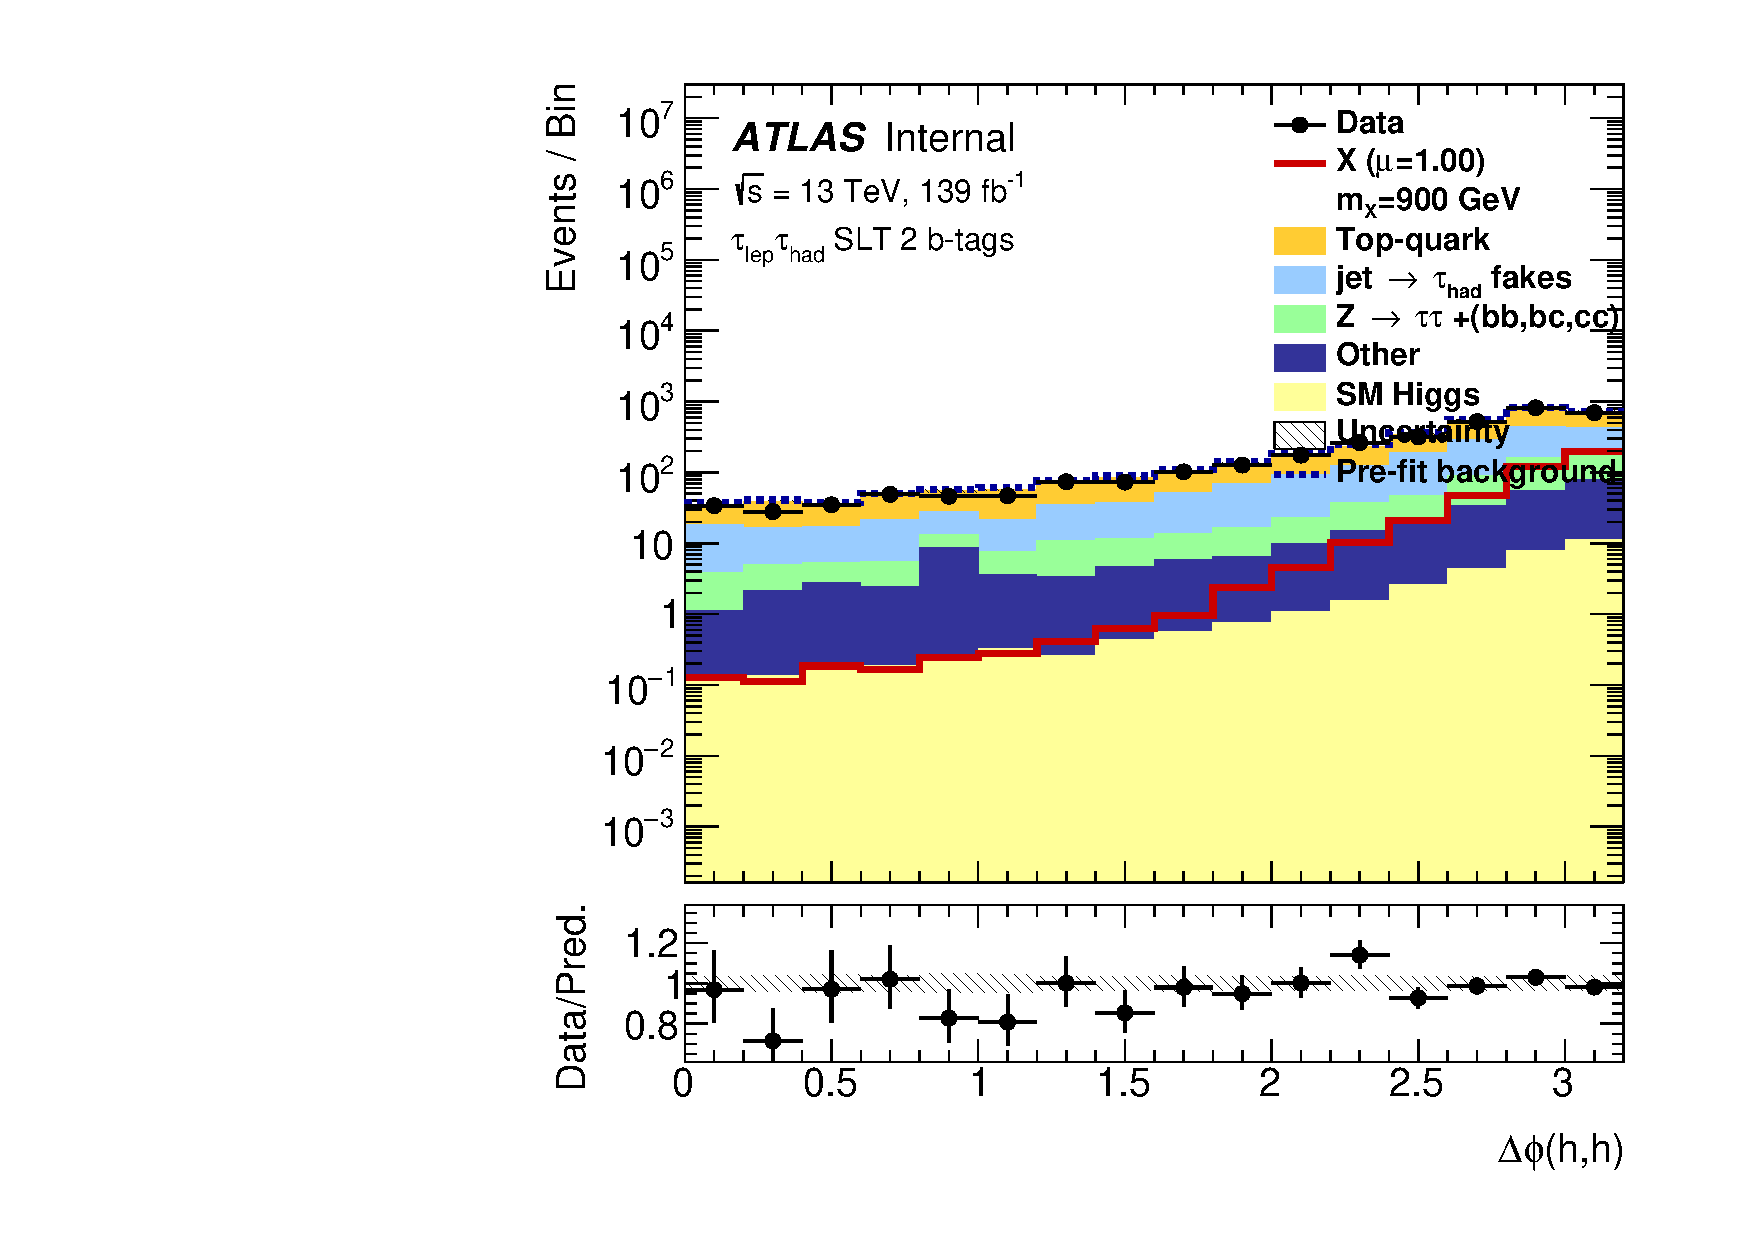
\includegraphics[width=.32\textwidth]{diHiggs/plots/MVA/postfit/Region_BMin0_incJet1_distdPhiHBB_J2_D_T2_SpcTauLH_Y2015_LTT0_L1_GlobalFit_conditionnal_mu0log.pdf} \\
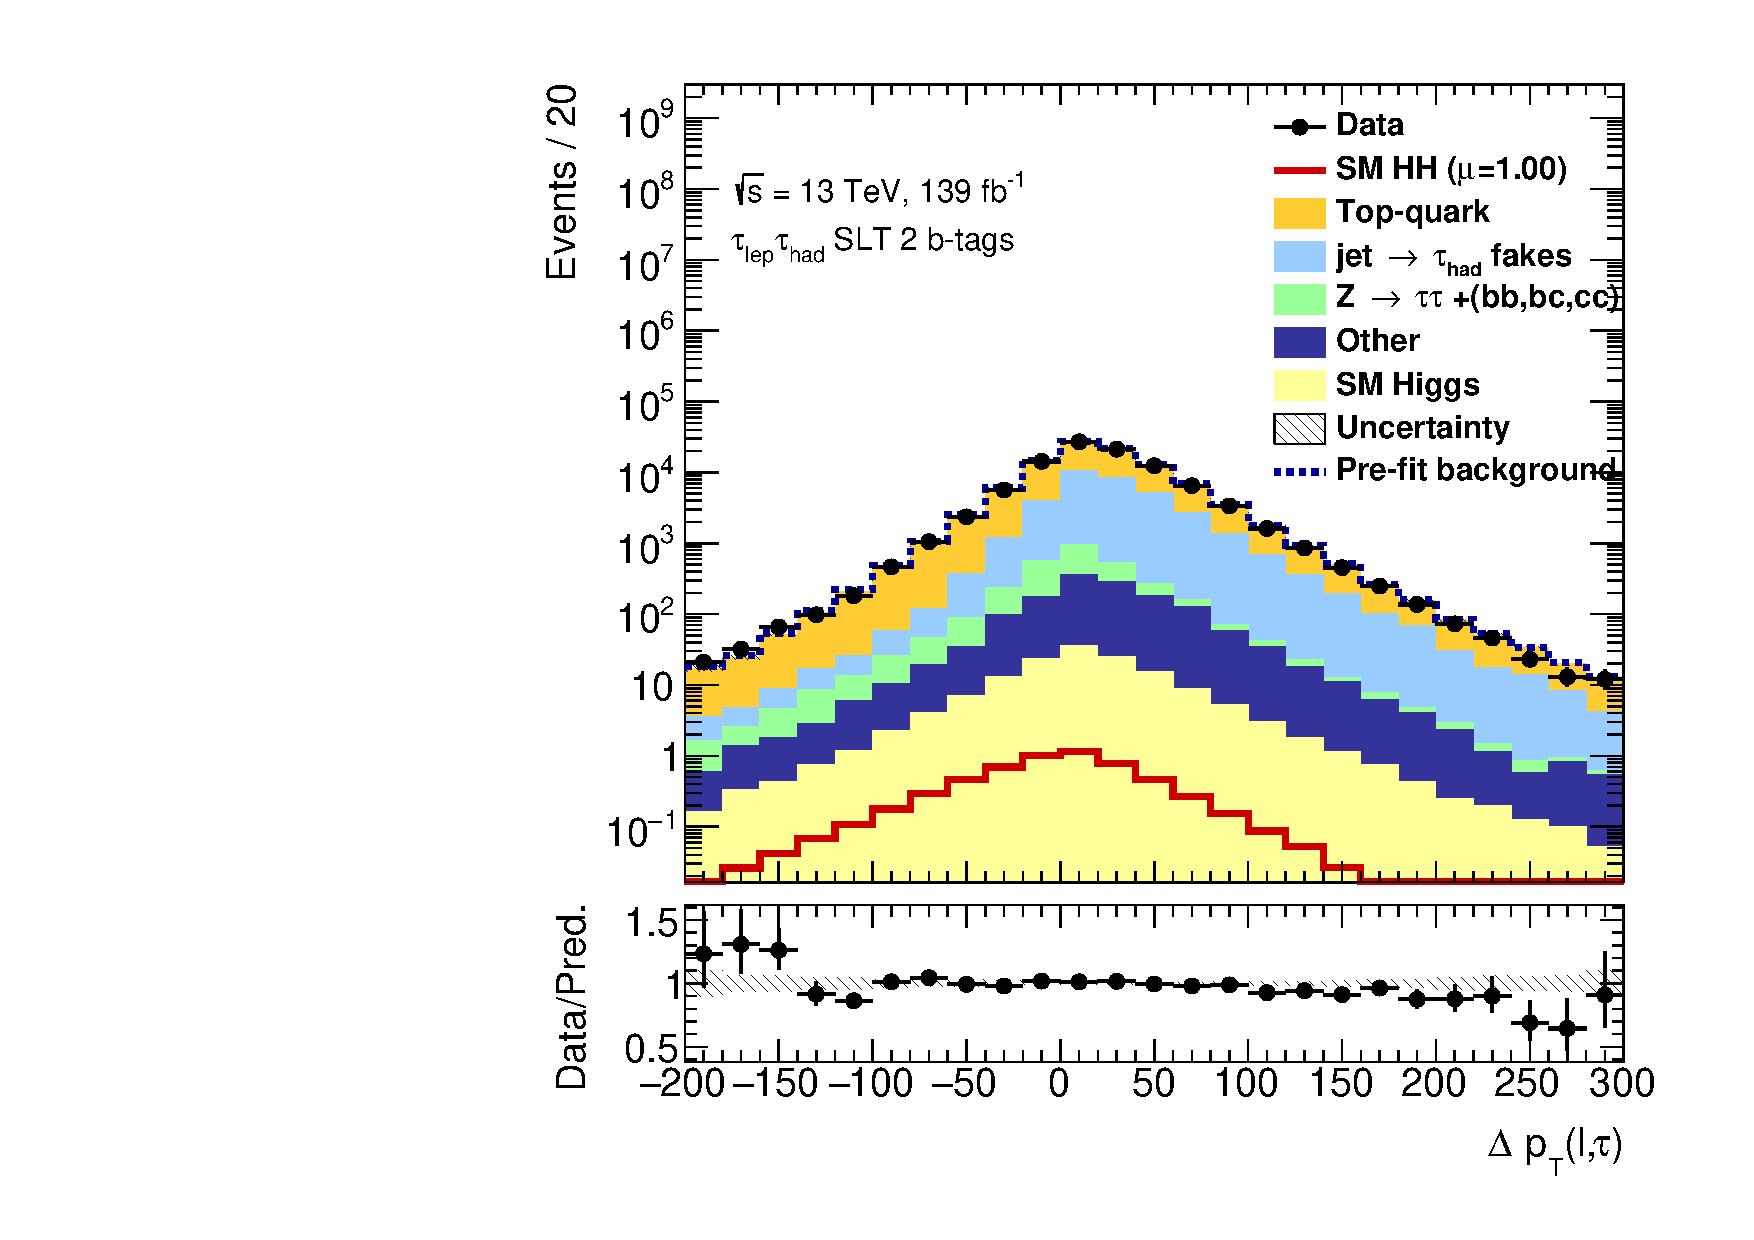
\includegraphics[width=.32\textwidth]{diHiggs/plots/MVA/postfit/Region_BMin0_incJet1_distdPtLepTau_J2_D_T2_SpcTauLH_Y2015_LTT0_L1_GlobalFit_conditionnal_mu0log.pdf}
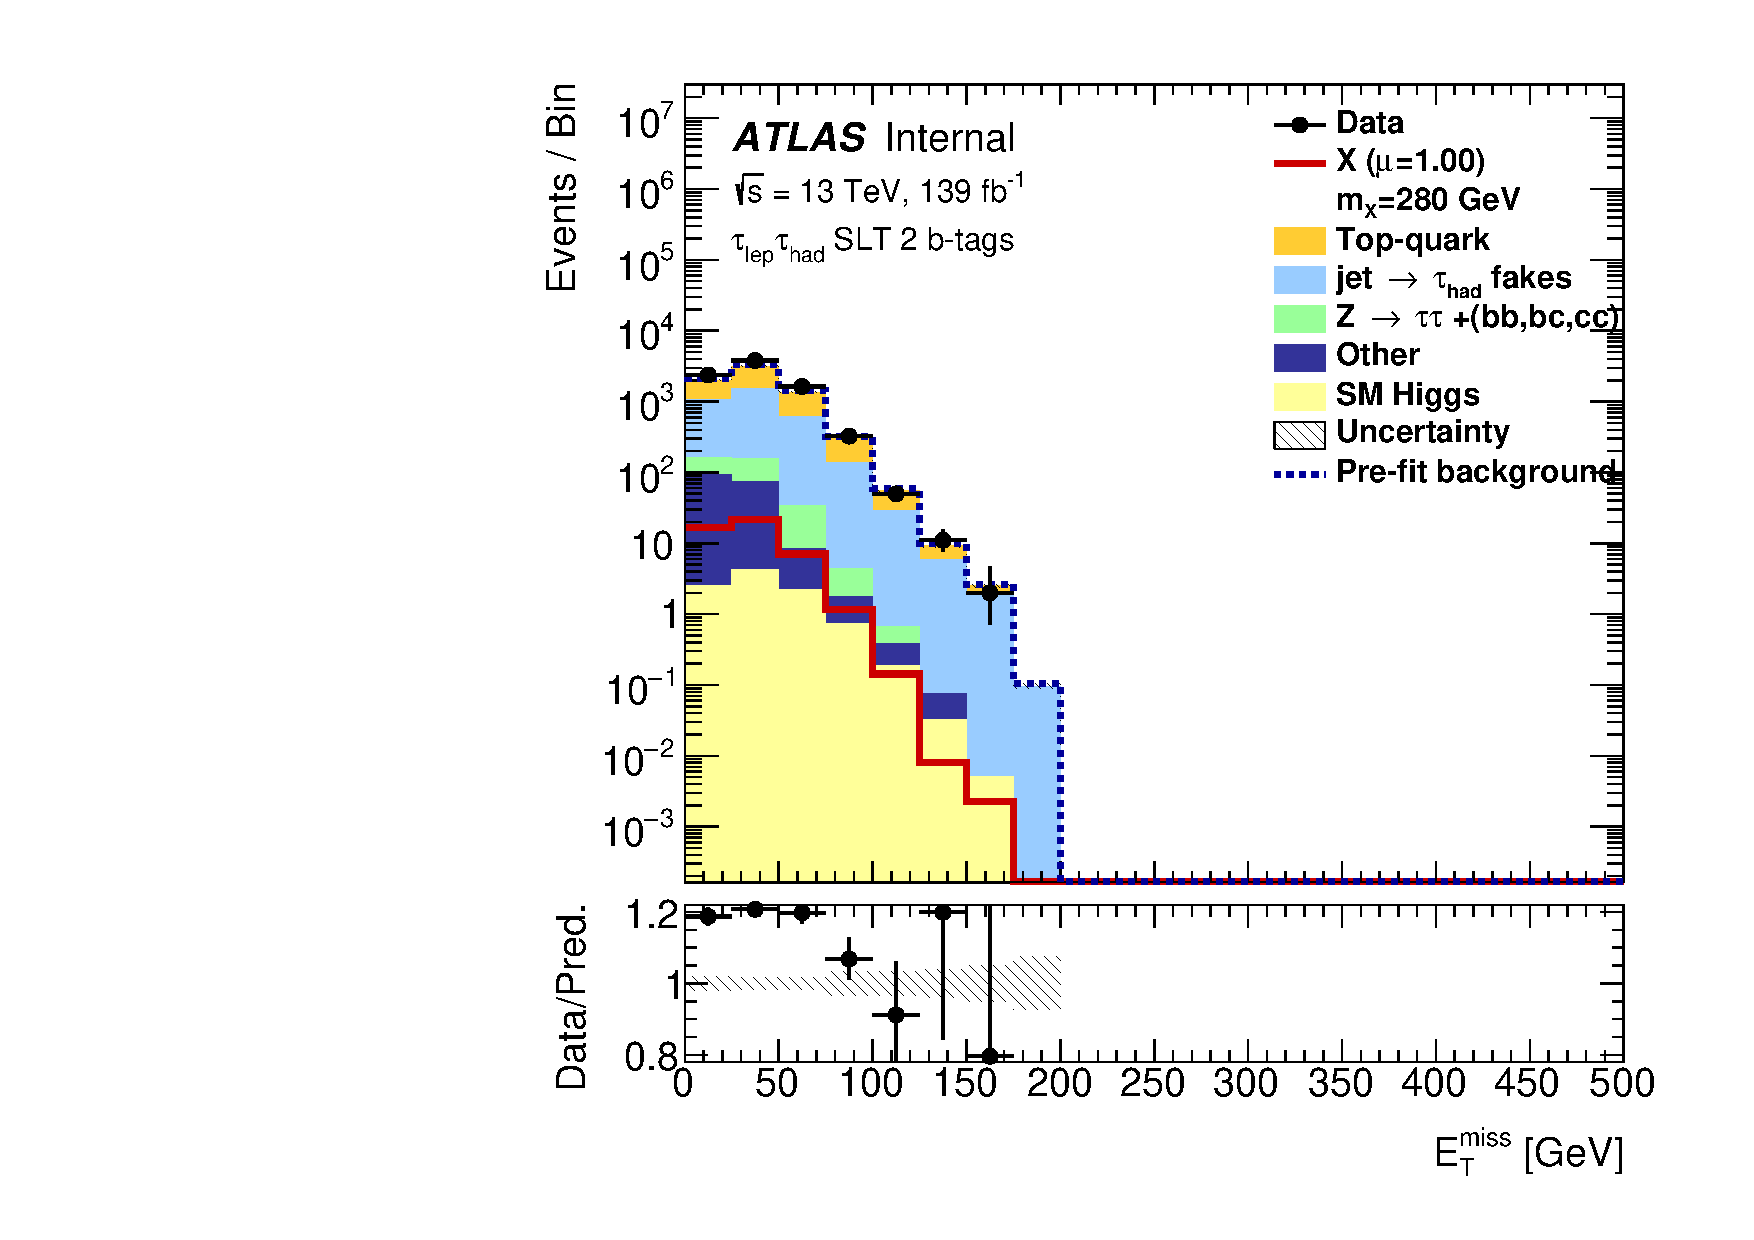
\includegraphics[width=.32\textwidth]{diHiggs/plots/MVA/postfit/Region_BMin0_incJet1_distMET_J2_D_T2_SpcTauLH_Y2015_LTT0_L1_GlobalFit_conditionnal_mu0log.pdf}
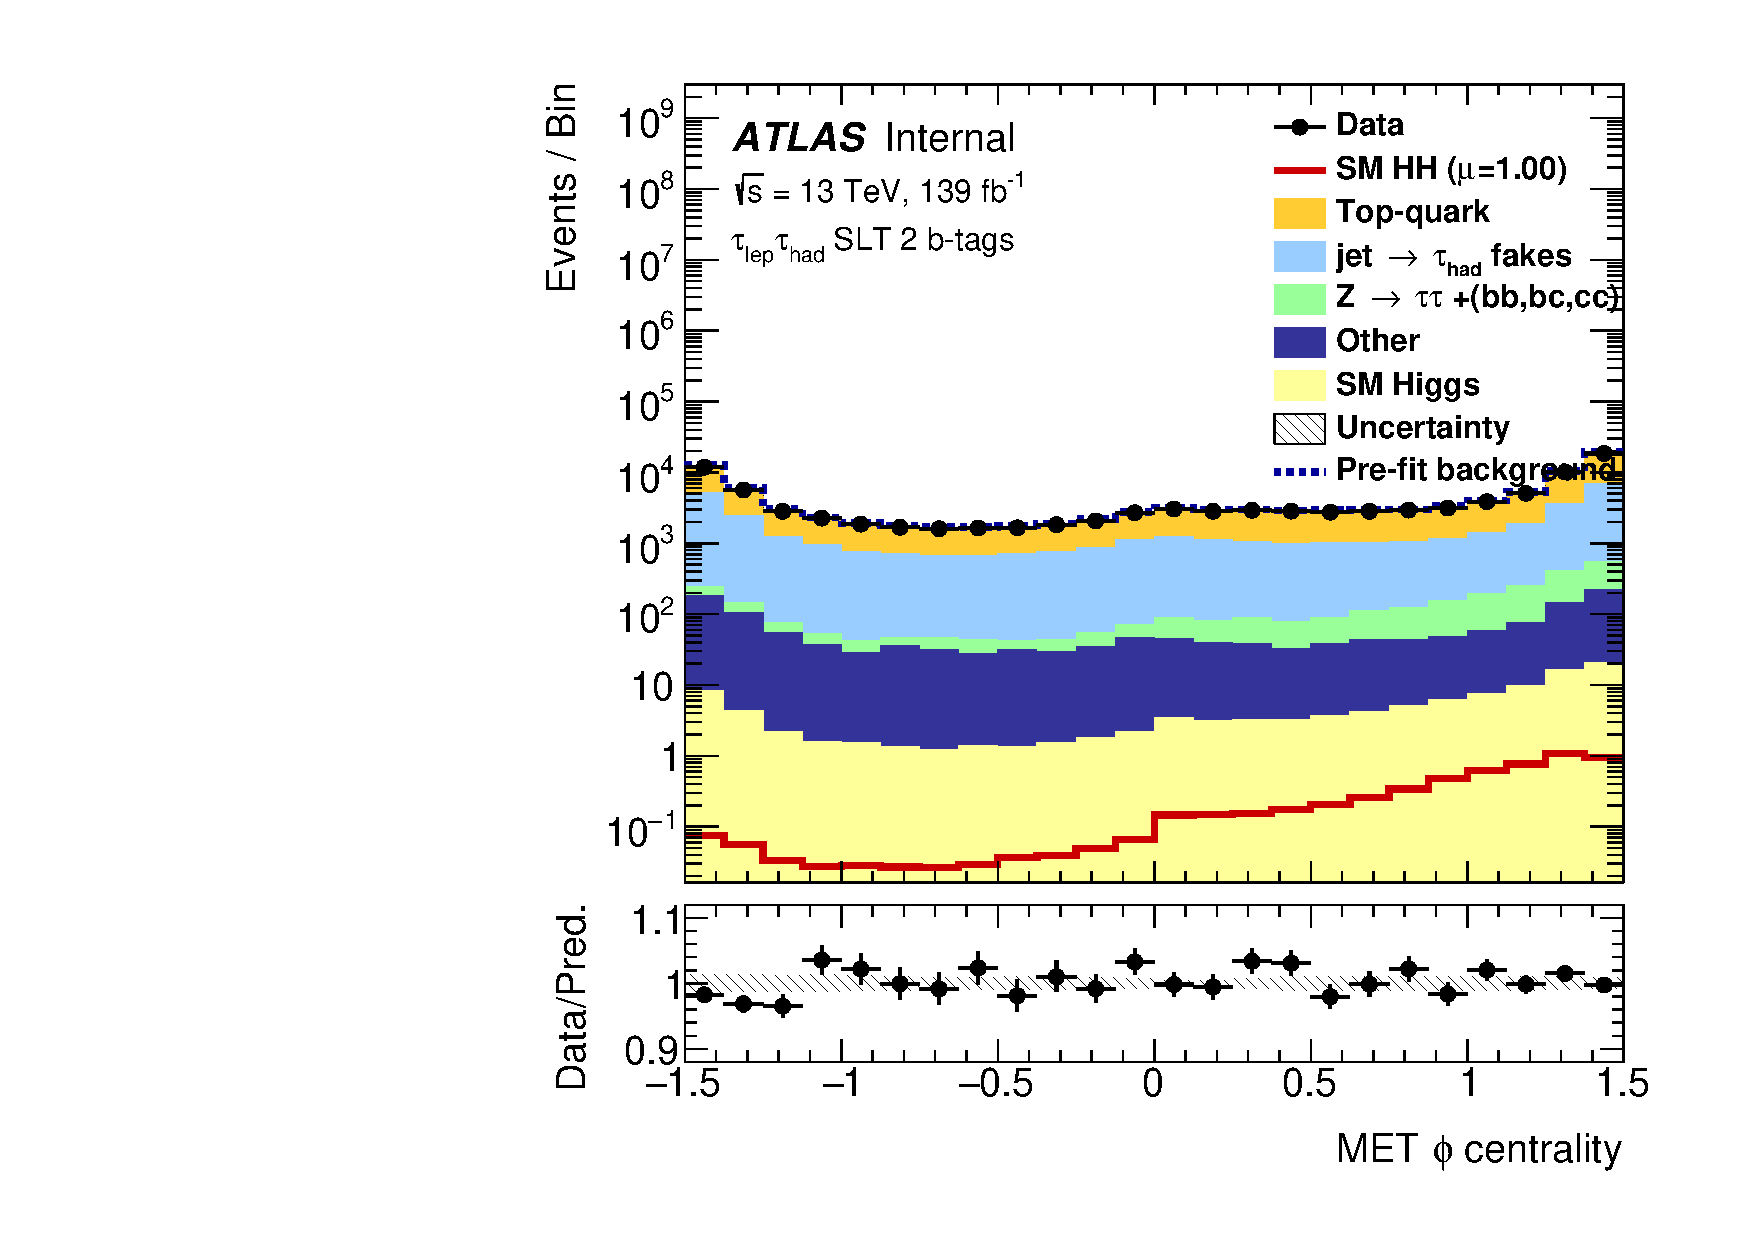
\includegraphics[width=.32\textwidth]{diHiggs/plots/MVA/postfit/Region_BMin0_incJet1_distMETCent_J2_D_T2_SpcTauLH_Y2015_LTT0_L1_GlobalFit_conditionnal_mu0log.pdf} \\
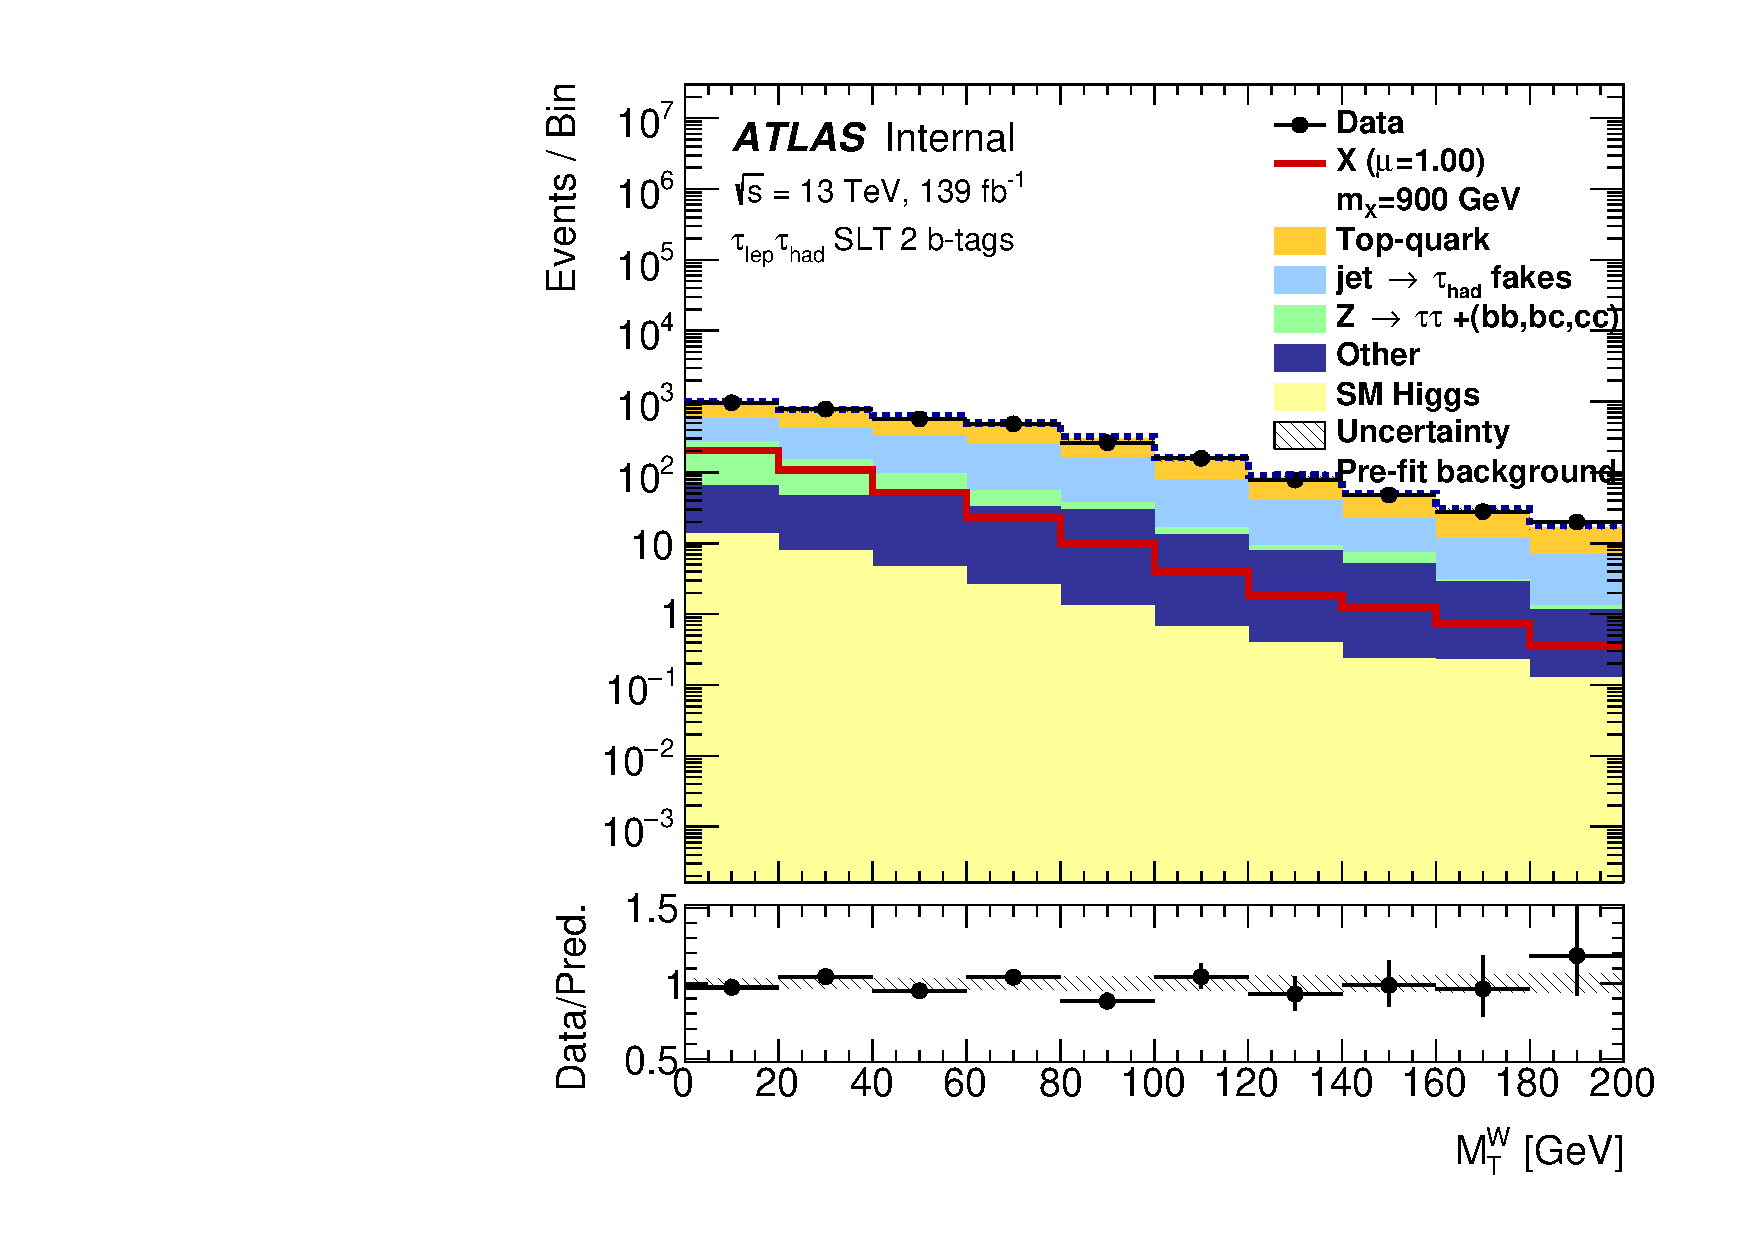
\includegraphics[width=.32\textwidth]{diHiggs/plots/MVA/postfit/Region_BMin0_incJet1_distMtW_J2_D_T2_SpcTauLH_Y2015_LTT0_L1_GlobalFit_conditionnal_mu0log.pdf}
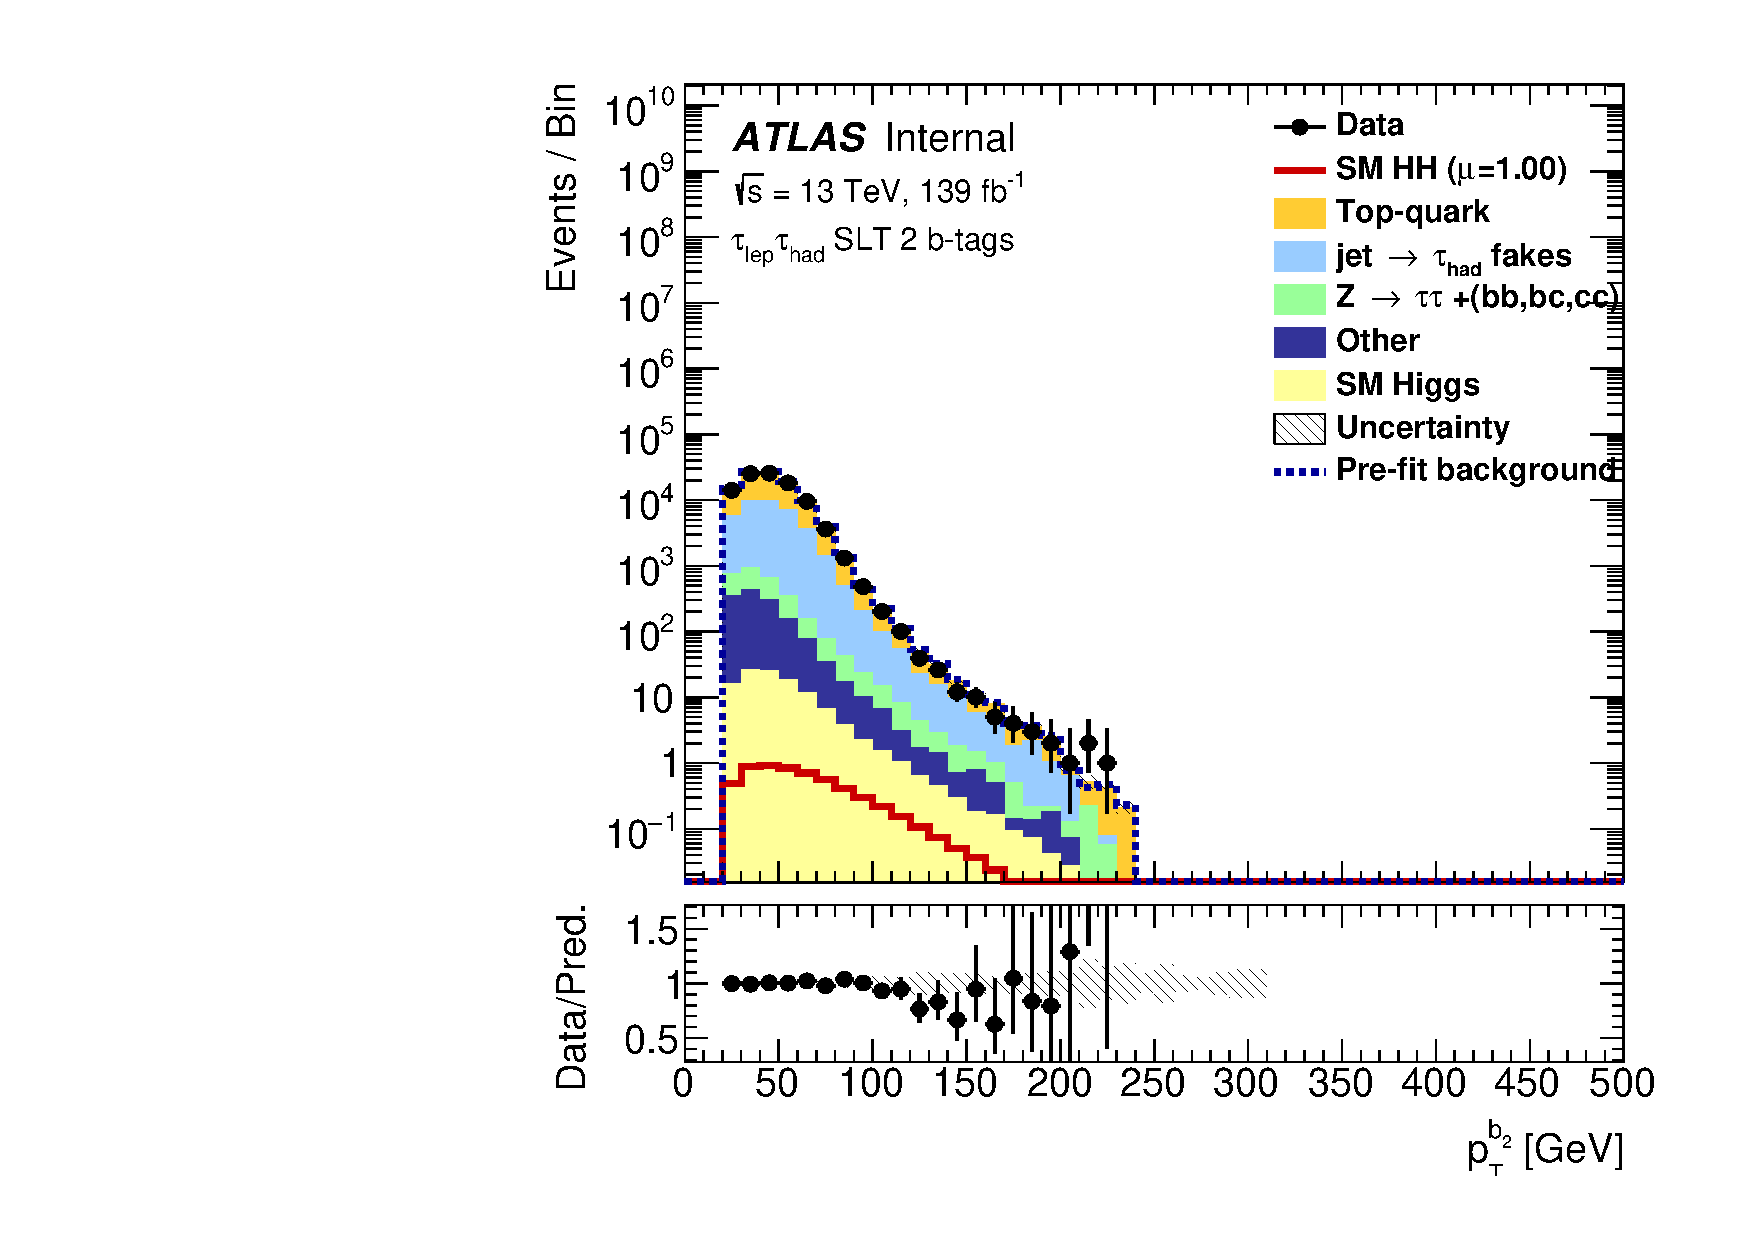
\includegraphics[width=.32\textwidth]{diHiggs/plots/MVA/postfit/Region_BMin0_incJet1_distpTB2_J2_D_T2_SpcTauLH_Y2015_LTT0_L1_GlobalFit_conditionnal_mu0log.pdf}
\caption{Post-fit PNN/NN input variable distributions in the SLT signal region.}
\label{fig:sltmvainputspostfit}
\end{figure}

\begin{figure}[htbp]
\centering
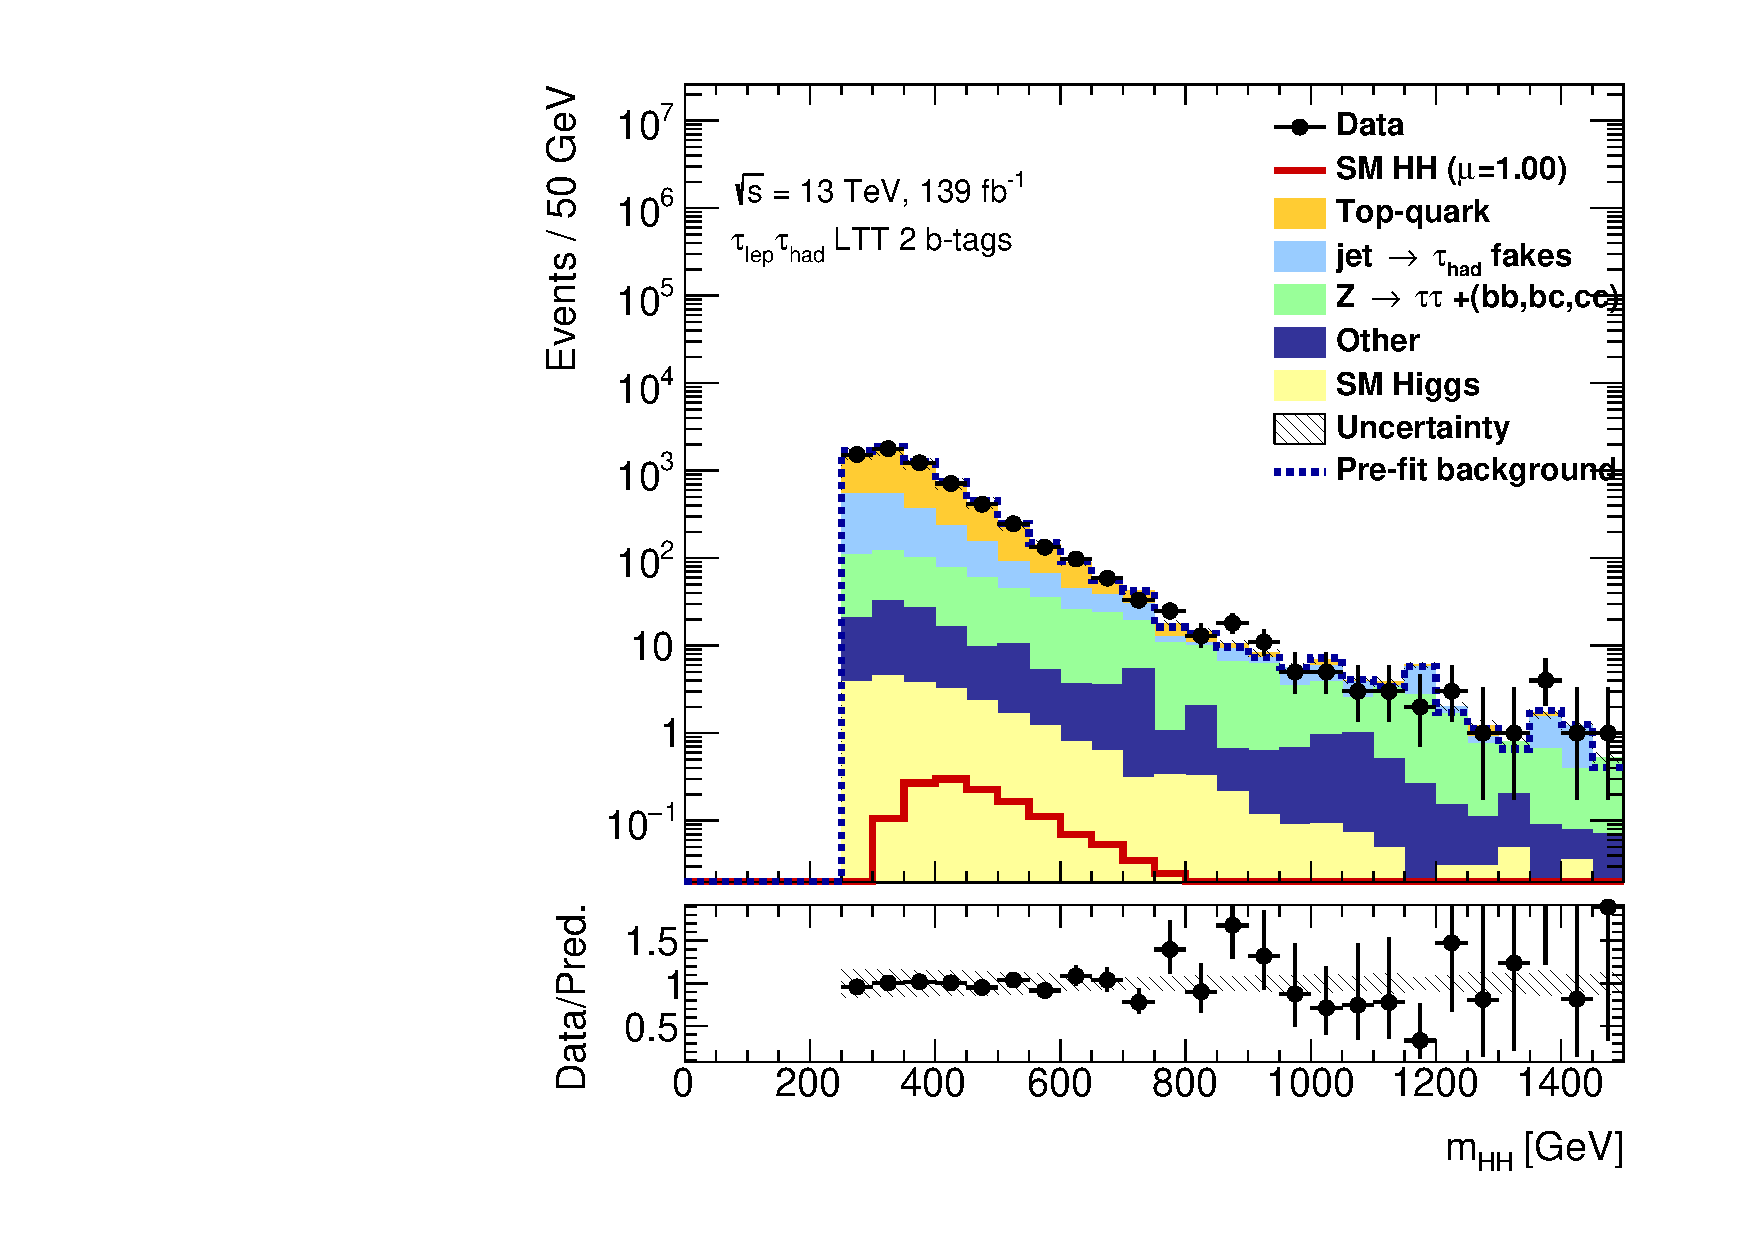
\includegraphics[width=.32\textwidth]{diHiggs/plots/MVA/postfit/Region_BMin0_incJet1_distMhh_J2_D_T2_SpcTauLH_Y2015_LTT1_L1_GlobalFit_conditionnal_mu0log.pdf}
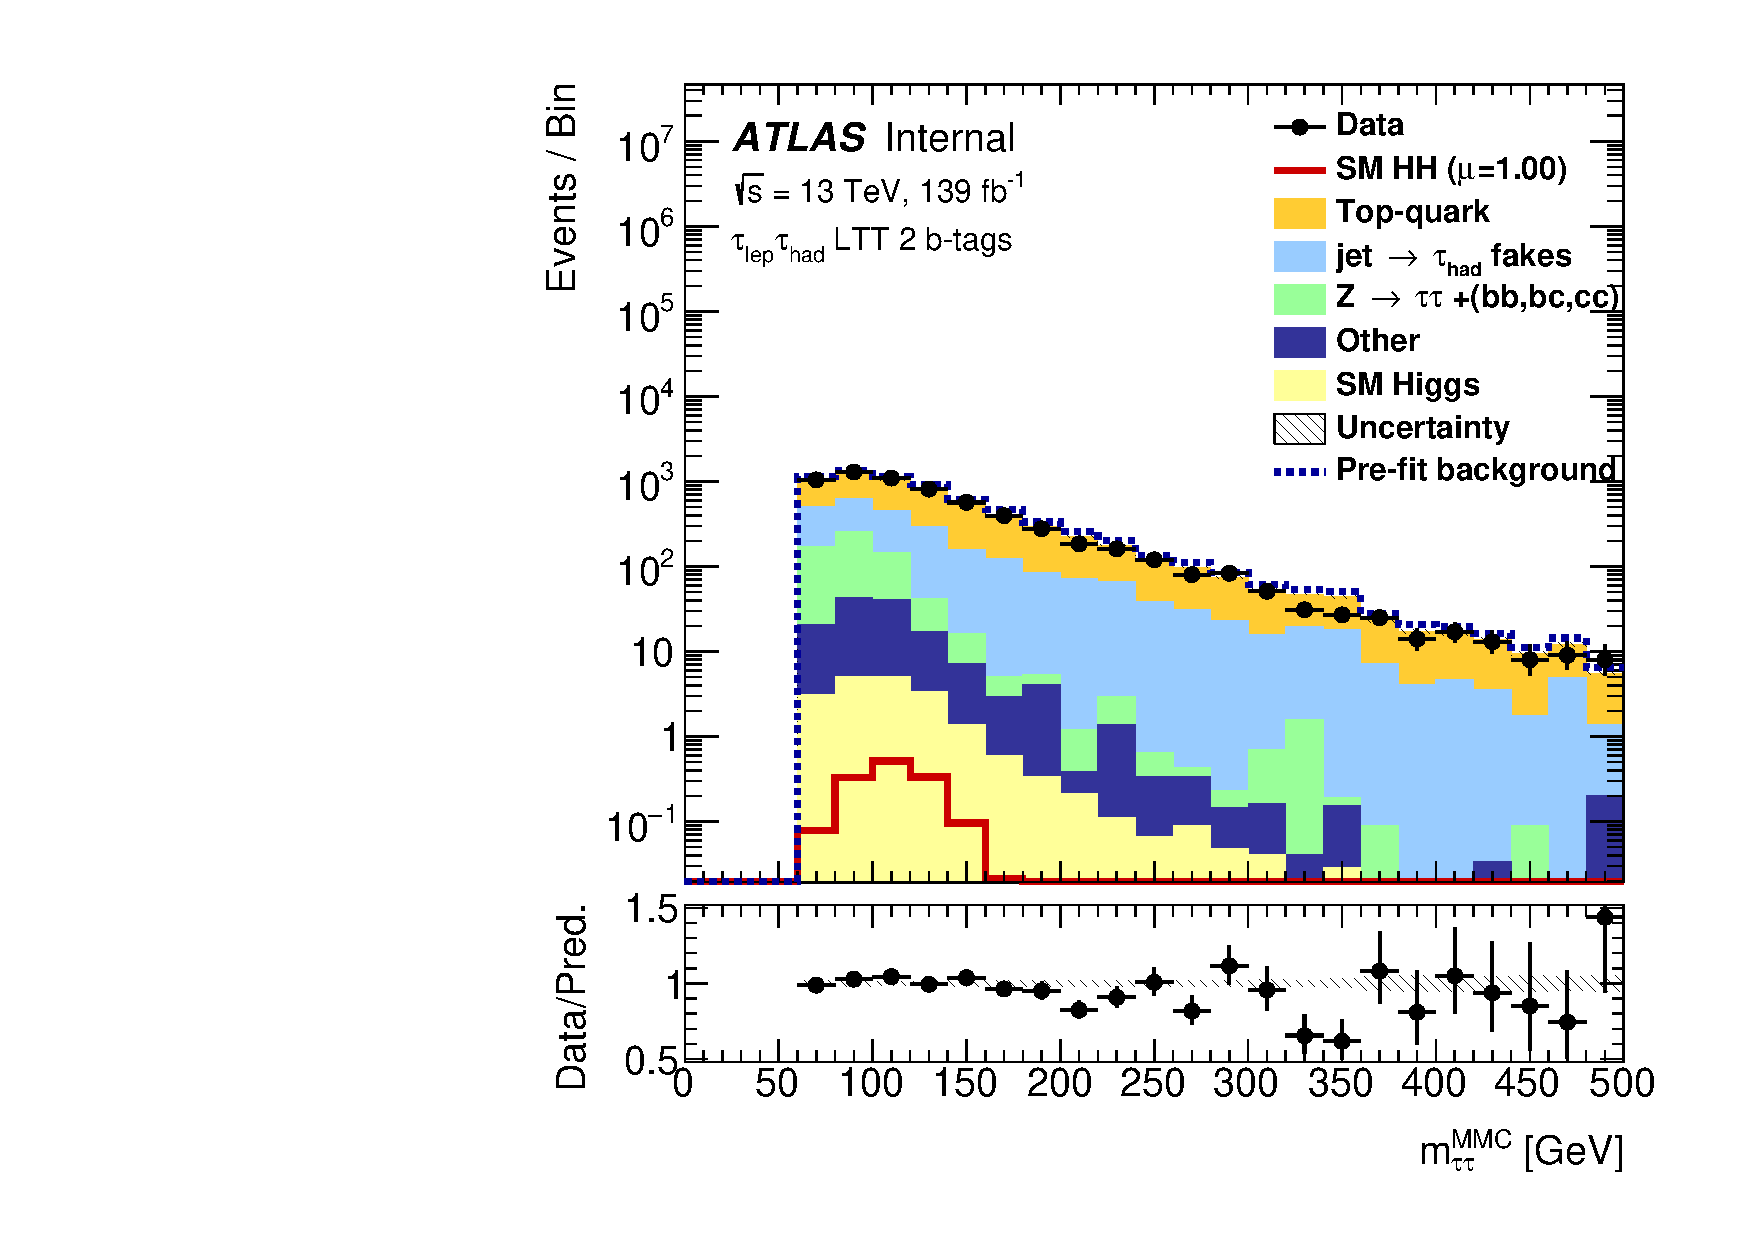
\includegraphics[width=.32\textwidth]{diHiggs/plots/MVA/postfit/Region_BMin0_incJet1_distmMMC_J2_D_T2_SpcTauLH_Y2015_LTT1_L1_GlobalFit_conditionnal_mu0log.pdf}
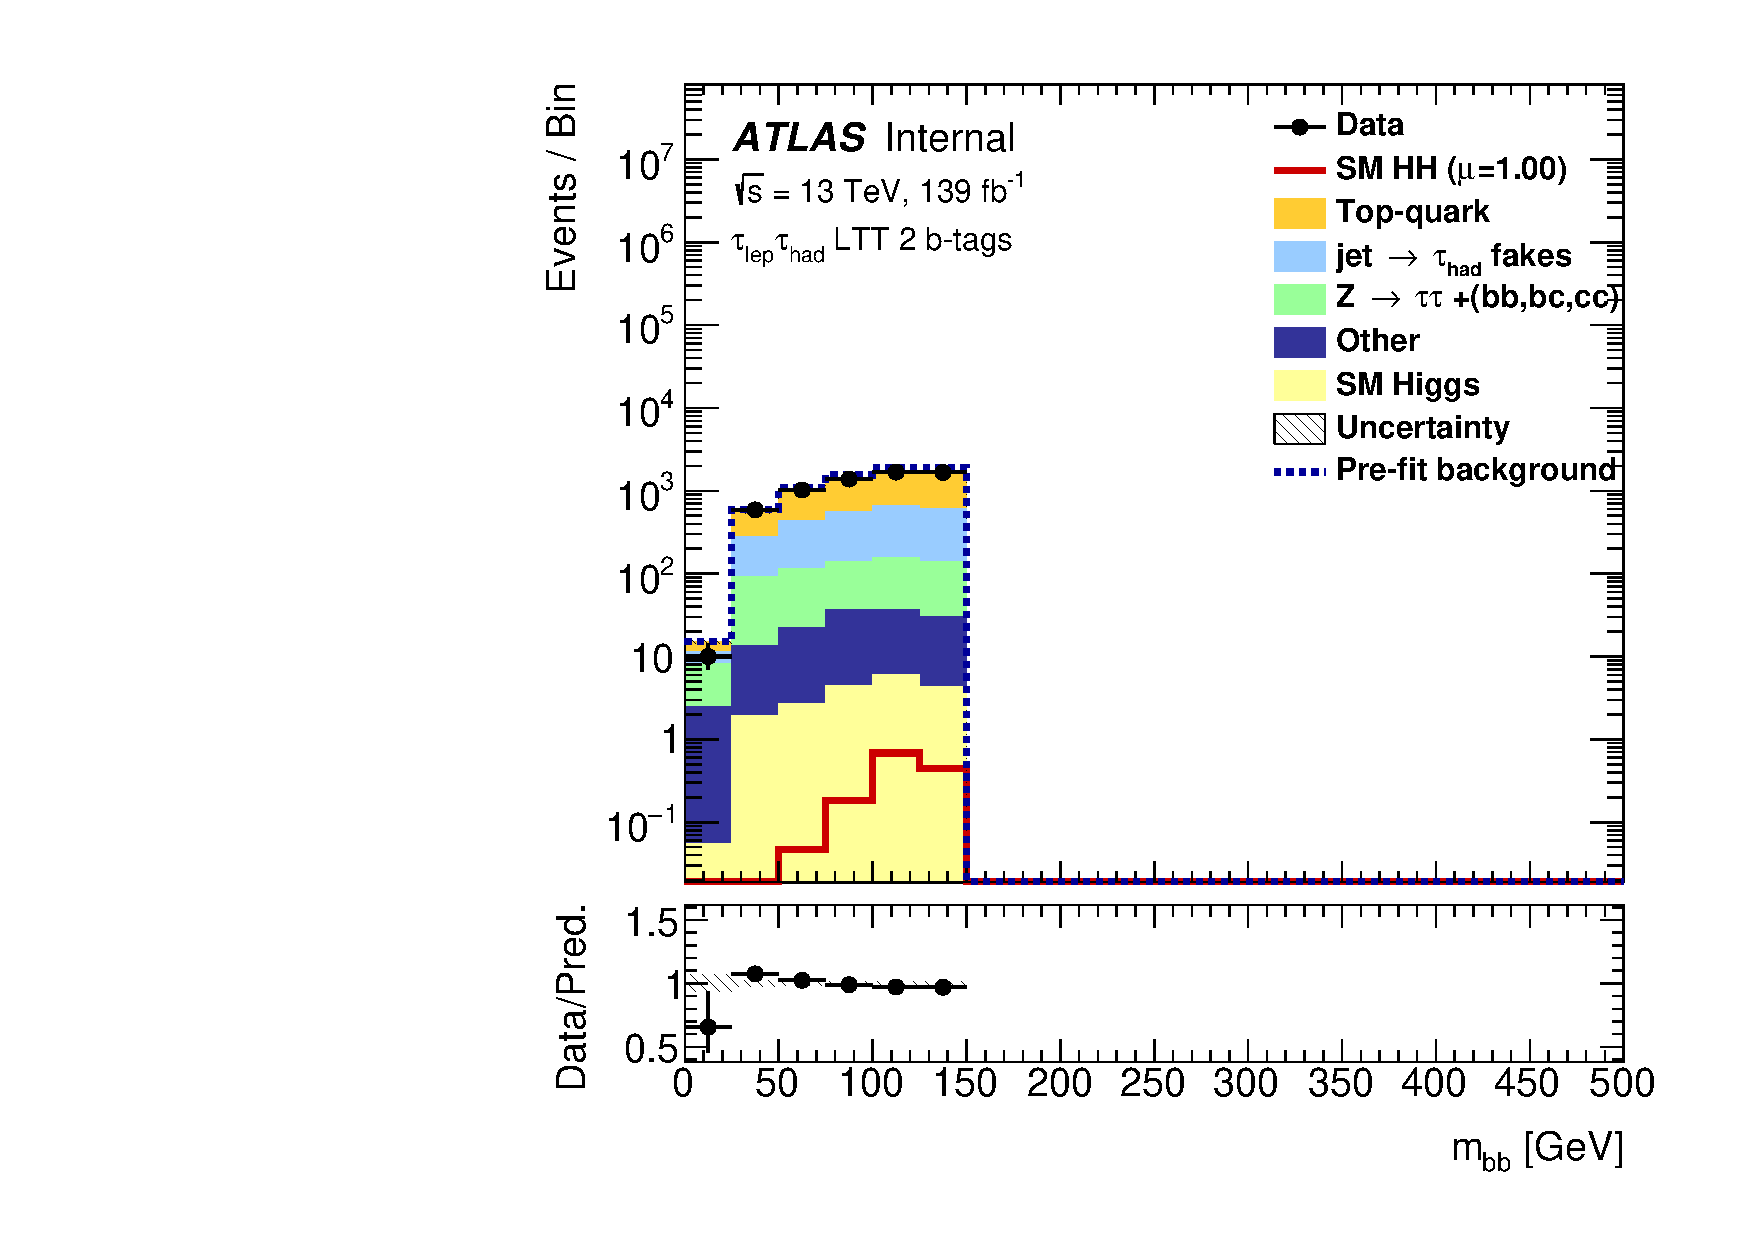
\includegraphics[width=.32\textwidth]{diHiggs/plots/MVA/postfit/Region_BMin0_incJet1_distmbb_J2_D_T2_SpcTauLH_Y2015_LTT1_L1_GlobalFit_conditionnal_mu0log.pdf} \\
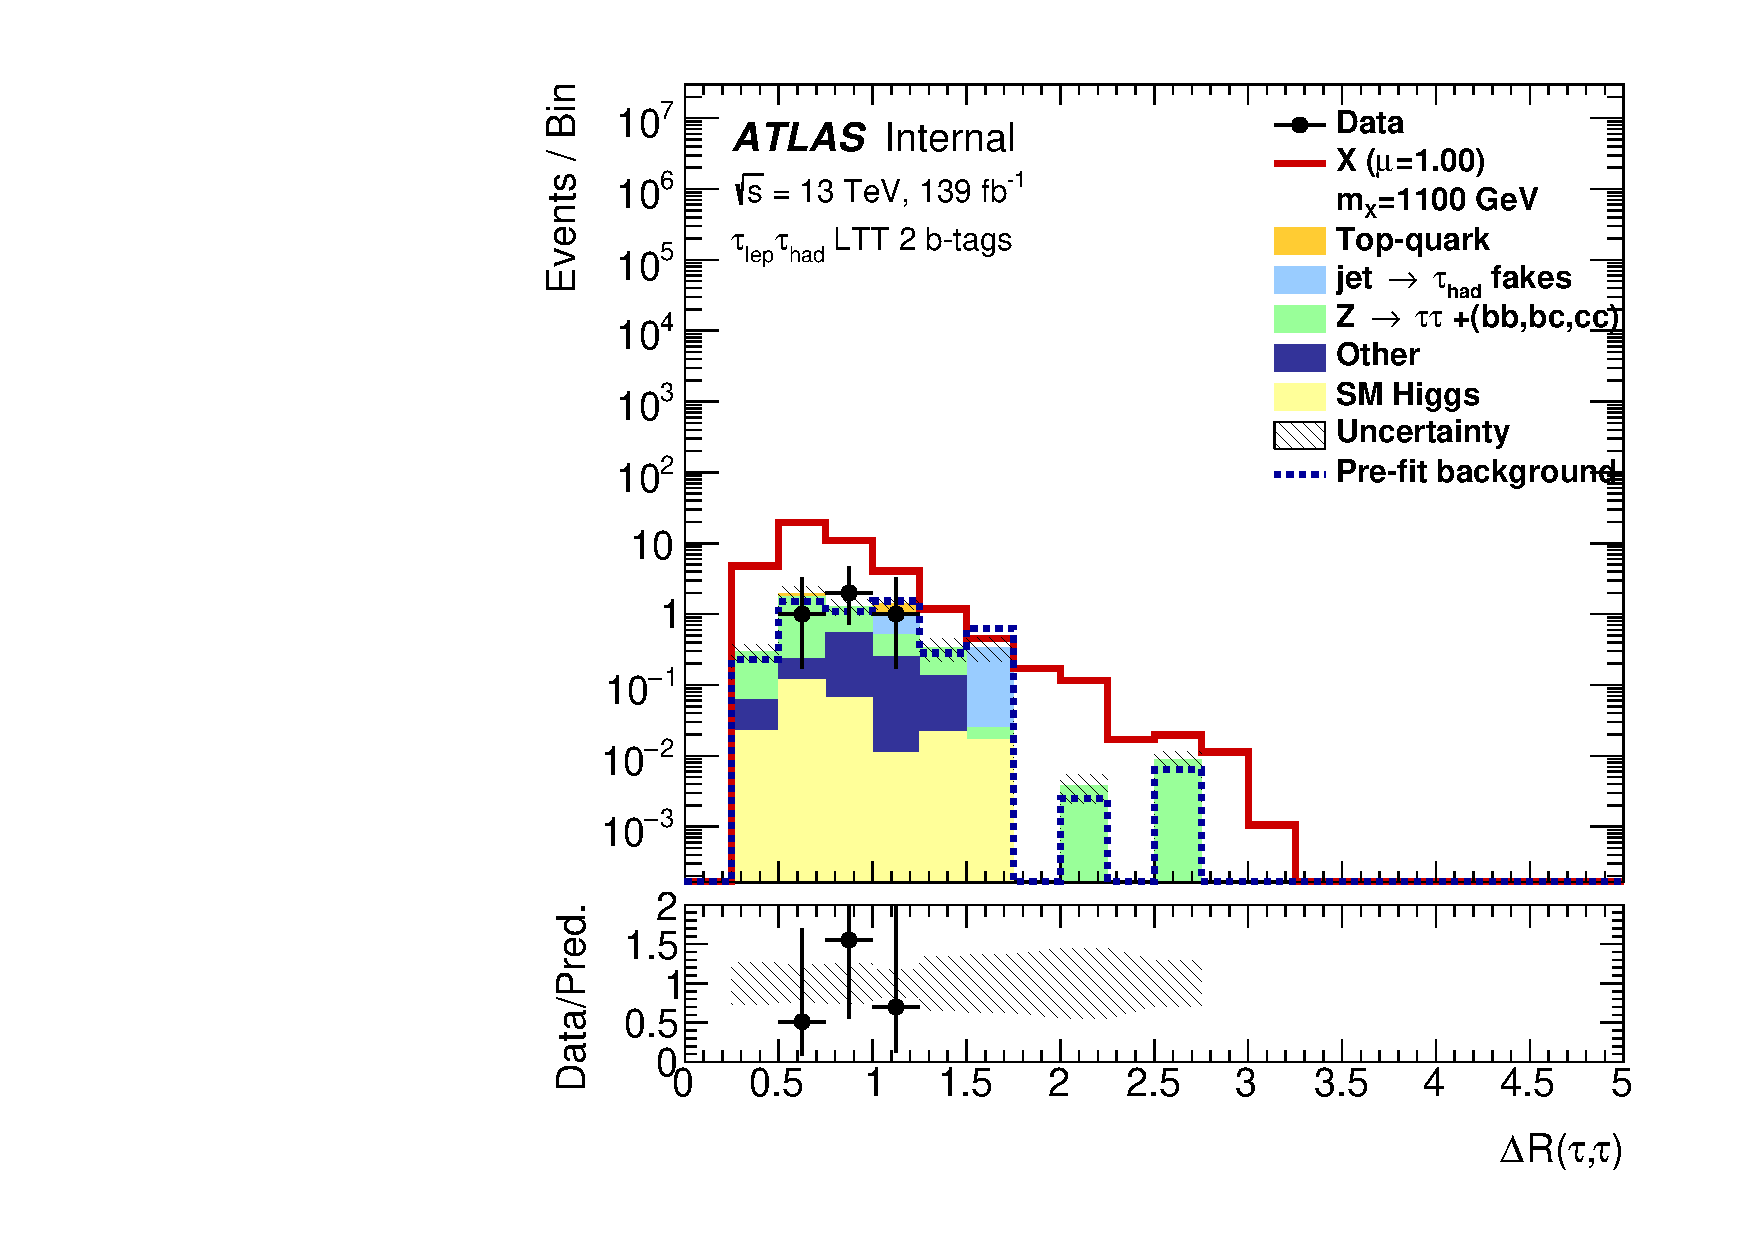
\includegraphics[width=.32\textwidth]{diHiggs/plots/MVA/postfit/Region_BMin0_incJet1_distDRTauTau_J2_D_T2_SpcTauLH_Y2015_LTT1_L1_GlobalFit_conditionnal_mu0log.pdf}
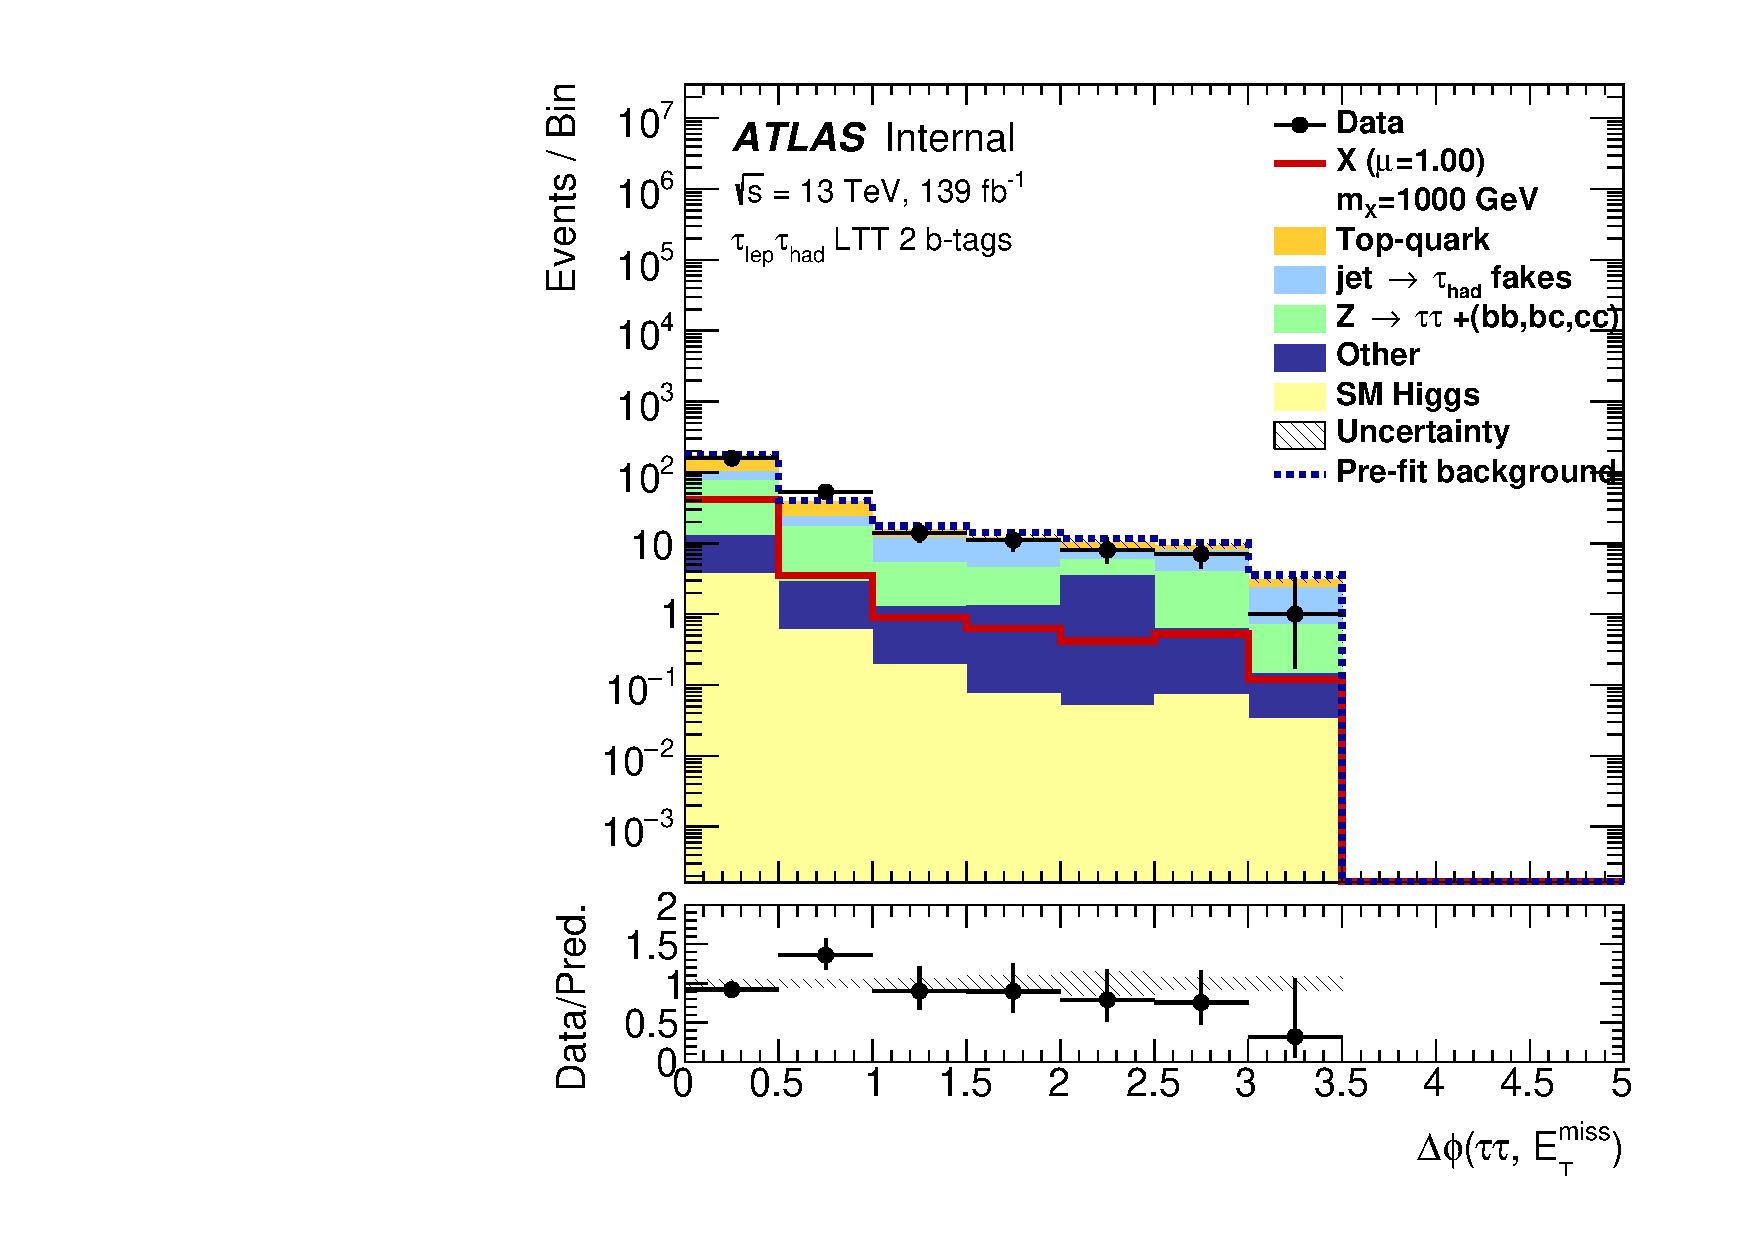
\includegraphics[width=.32\textwidth]{diHiggs/plots/MVA/postfit/Region_BMin0_incJet1_distdPhiHttMET_J2_D_T2_SpcTauLH_Y2015_LTT1_L1_GlobalFit_conditionnal_mu0log.pdf}
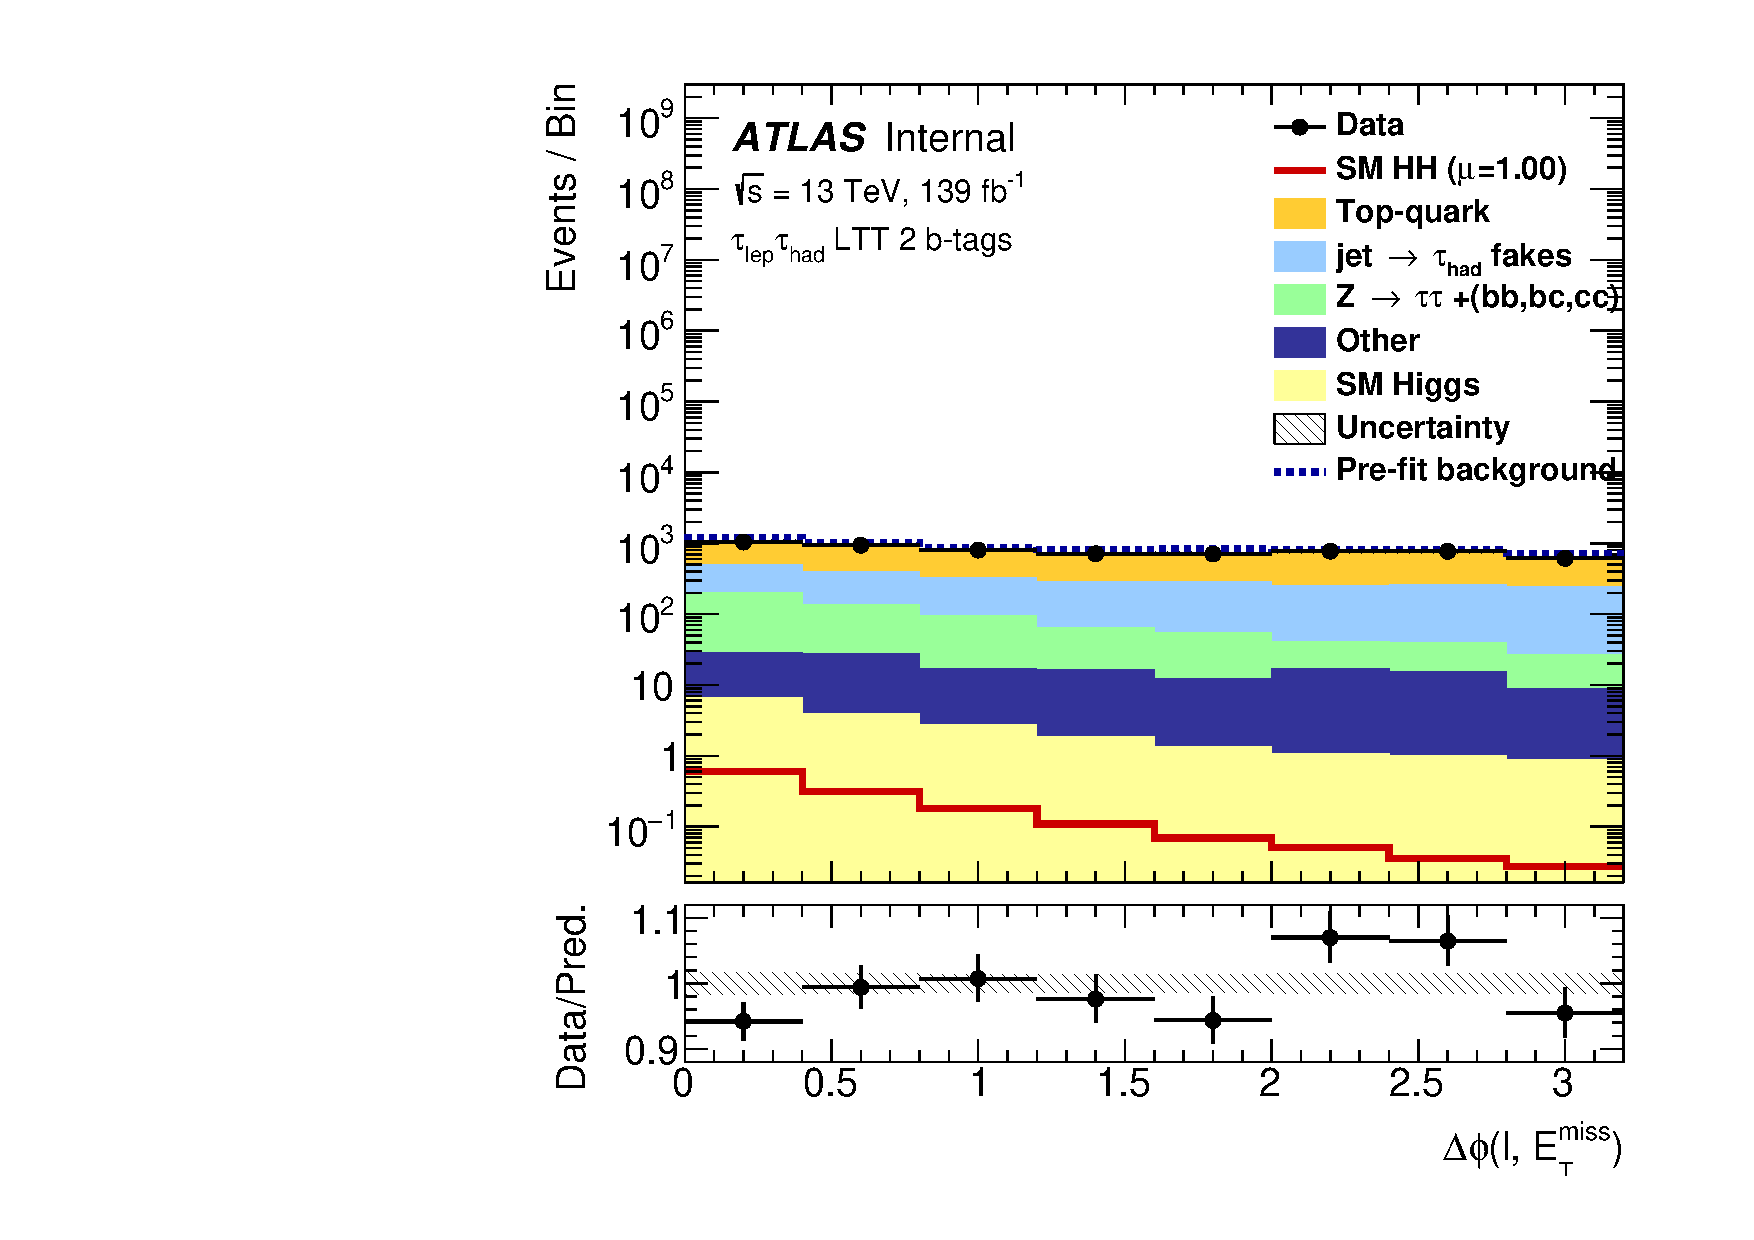
\includegraphics[width=.32\textwidth]{diHiggs/plots/MVA/postfit/Region_BMin0_incJet1_distdPhiLep0MET_J2_D_T2_SpcTauLH_Y2015_LTT1_L1_GlobalFit_conditionnal_mu0log.pdf} \\
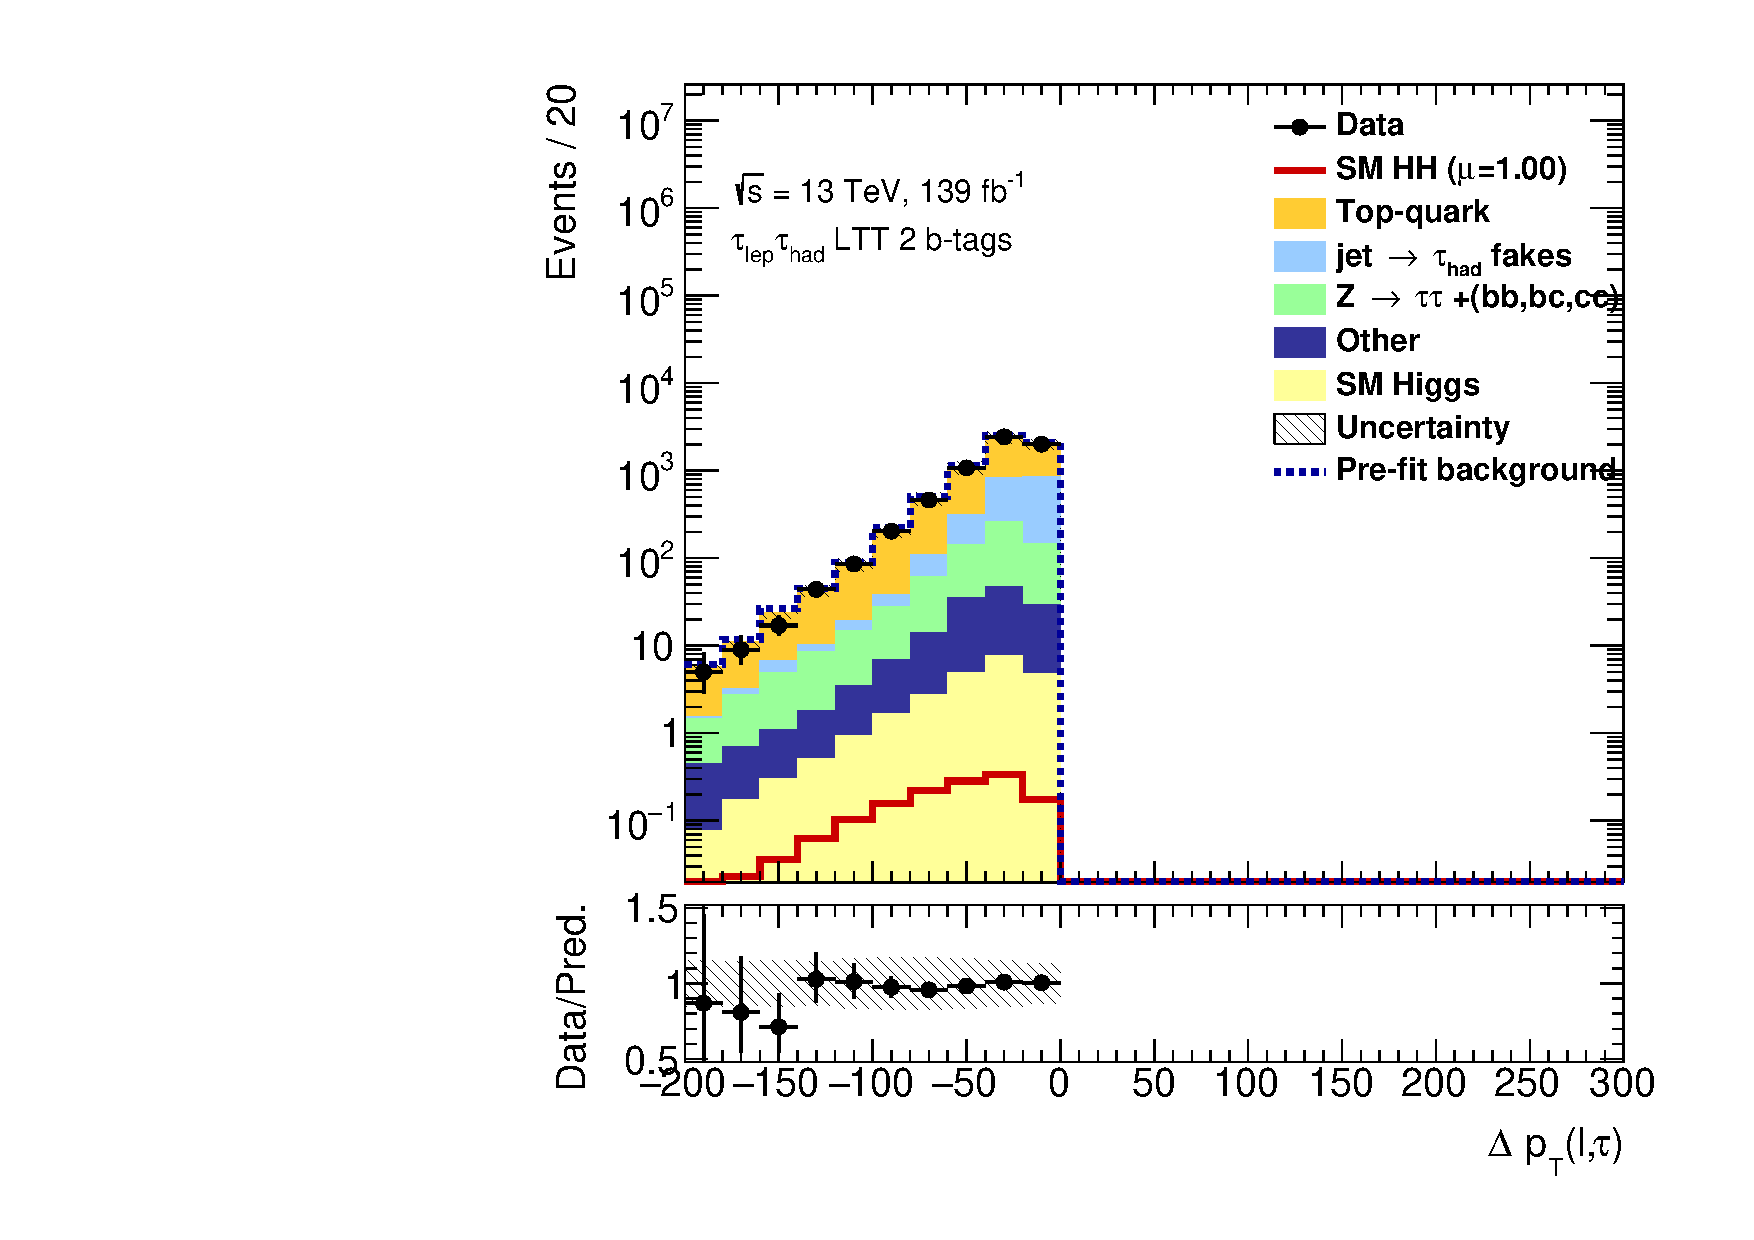
\includegraphics[width=.32\textwidth]{diHiggs/plots/MVA/postfit/Region_BMin0_incJet1_distdPtLepTau_J2_D_T2_SpcTauLH_Y2015_LTT1_L1_GlobalFit_conditionnal_mu0log.pdf}
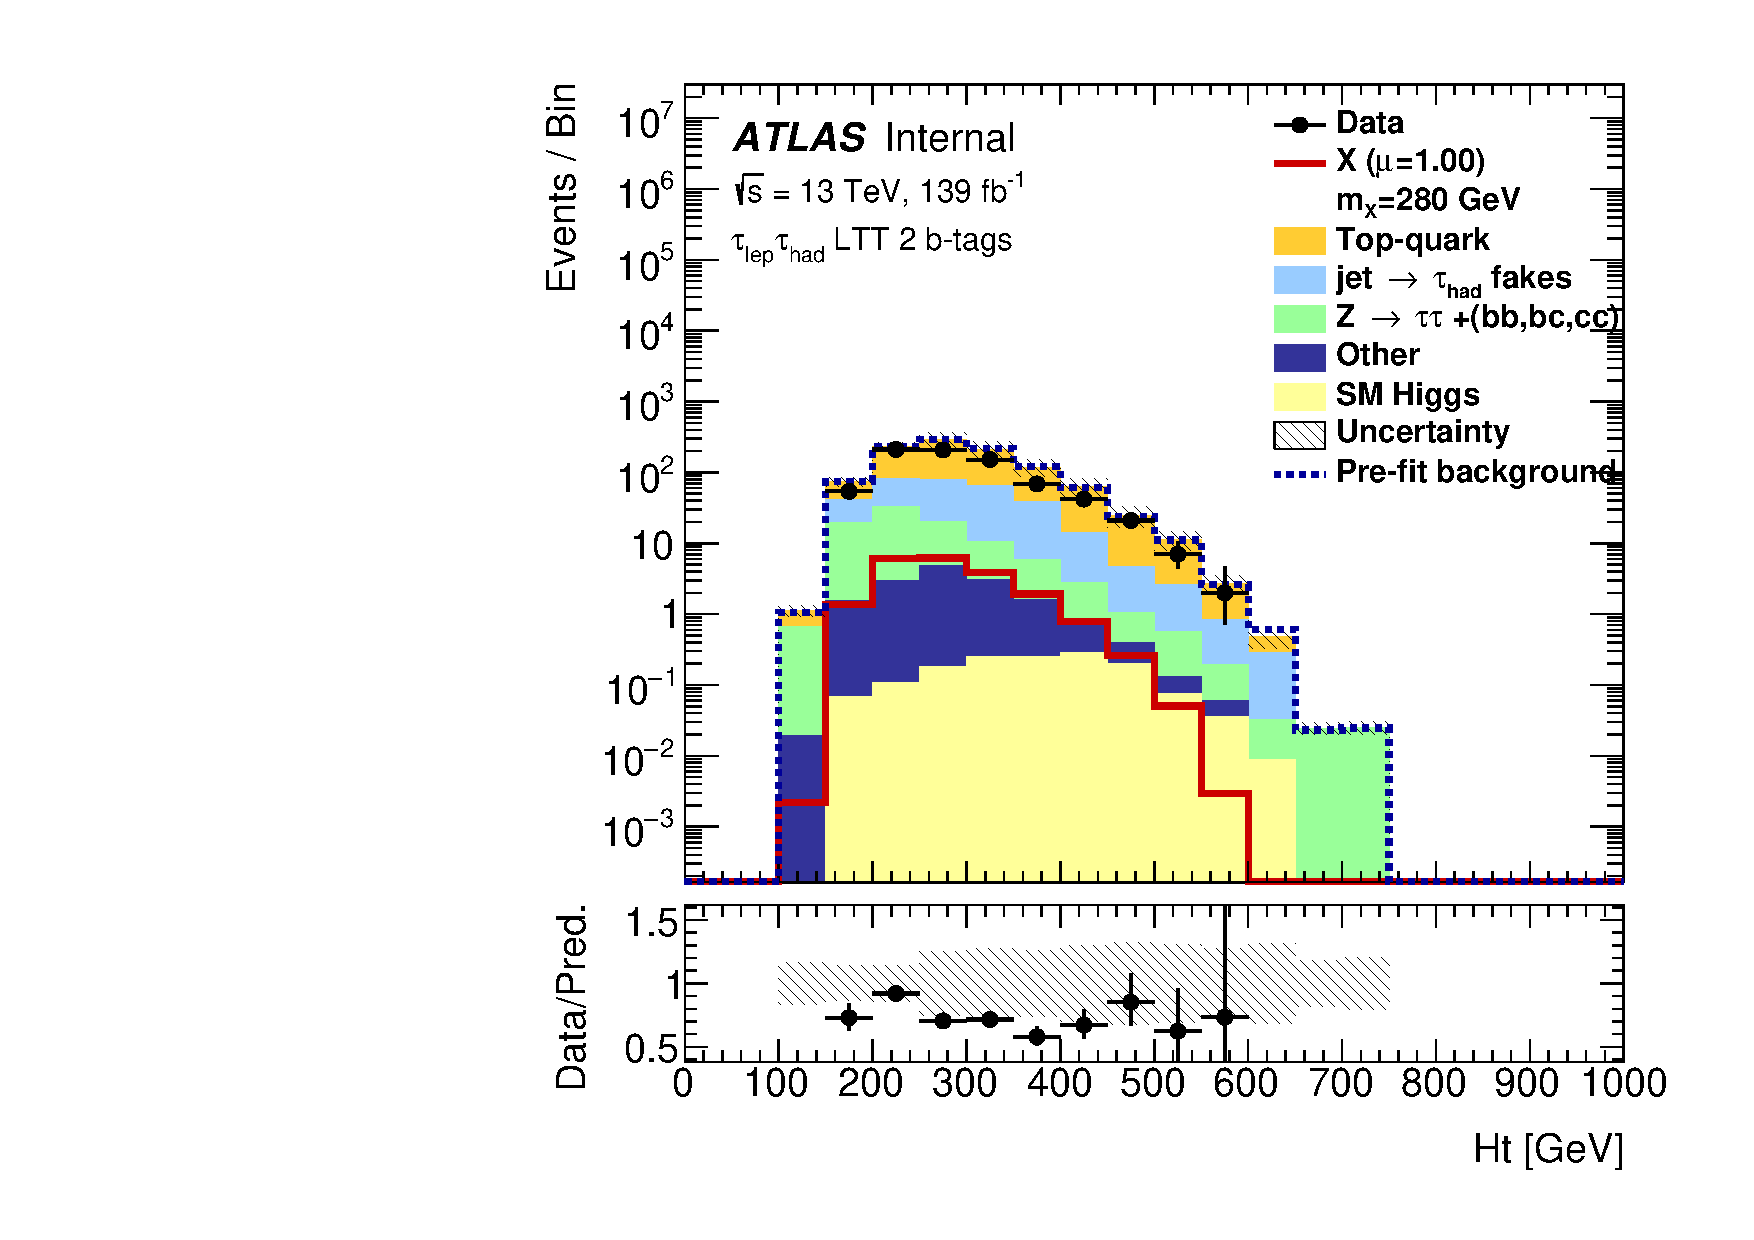
\includegraphics[width=.32\textwidth]{diHiggs/plots/MVA/postfit/Region_BMin0_incJet1_distHt_J2_D_T2_SpcTauLH_Y2015_LTT1_L1_GlobalFit_conditionnal_mu0log.pdf}
\caption{Post-fit PNN/NN input variable distributions in the LTT signal region.}
\label{fig:lttmvainputspostfit}
\end{figure}


% \begin{figure}[htbp]
% \centering
% \subfloat[]
%    {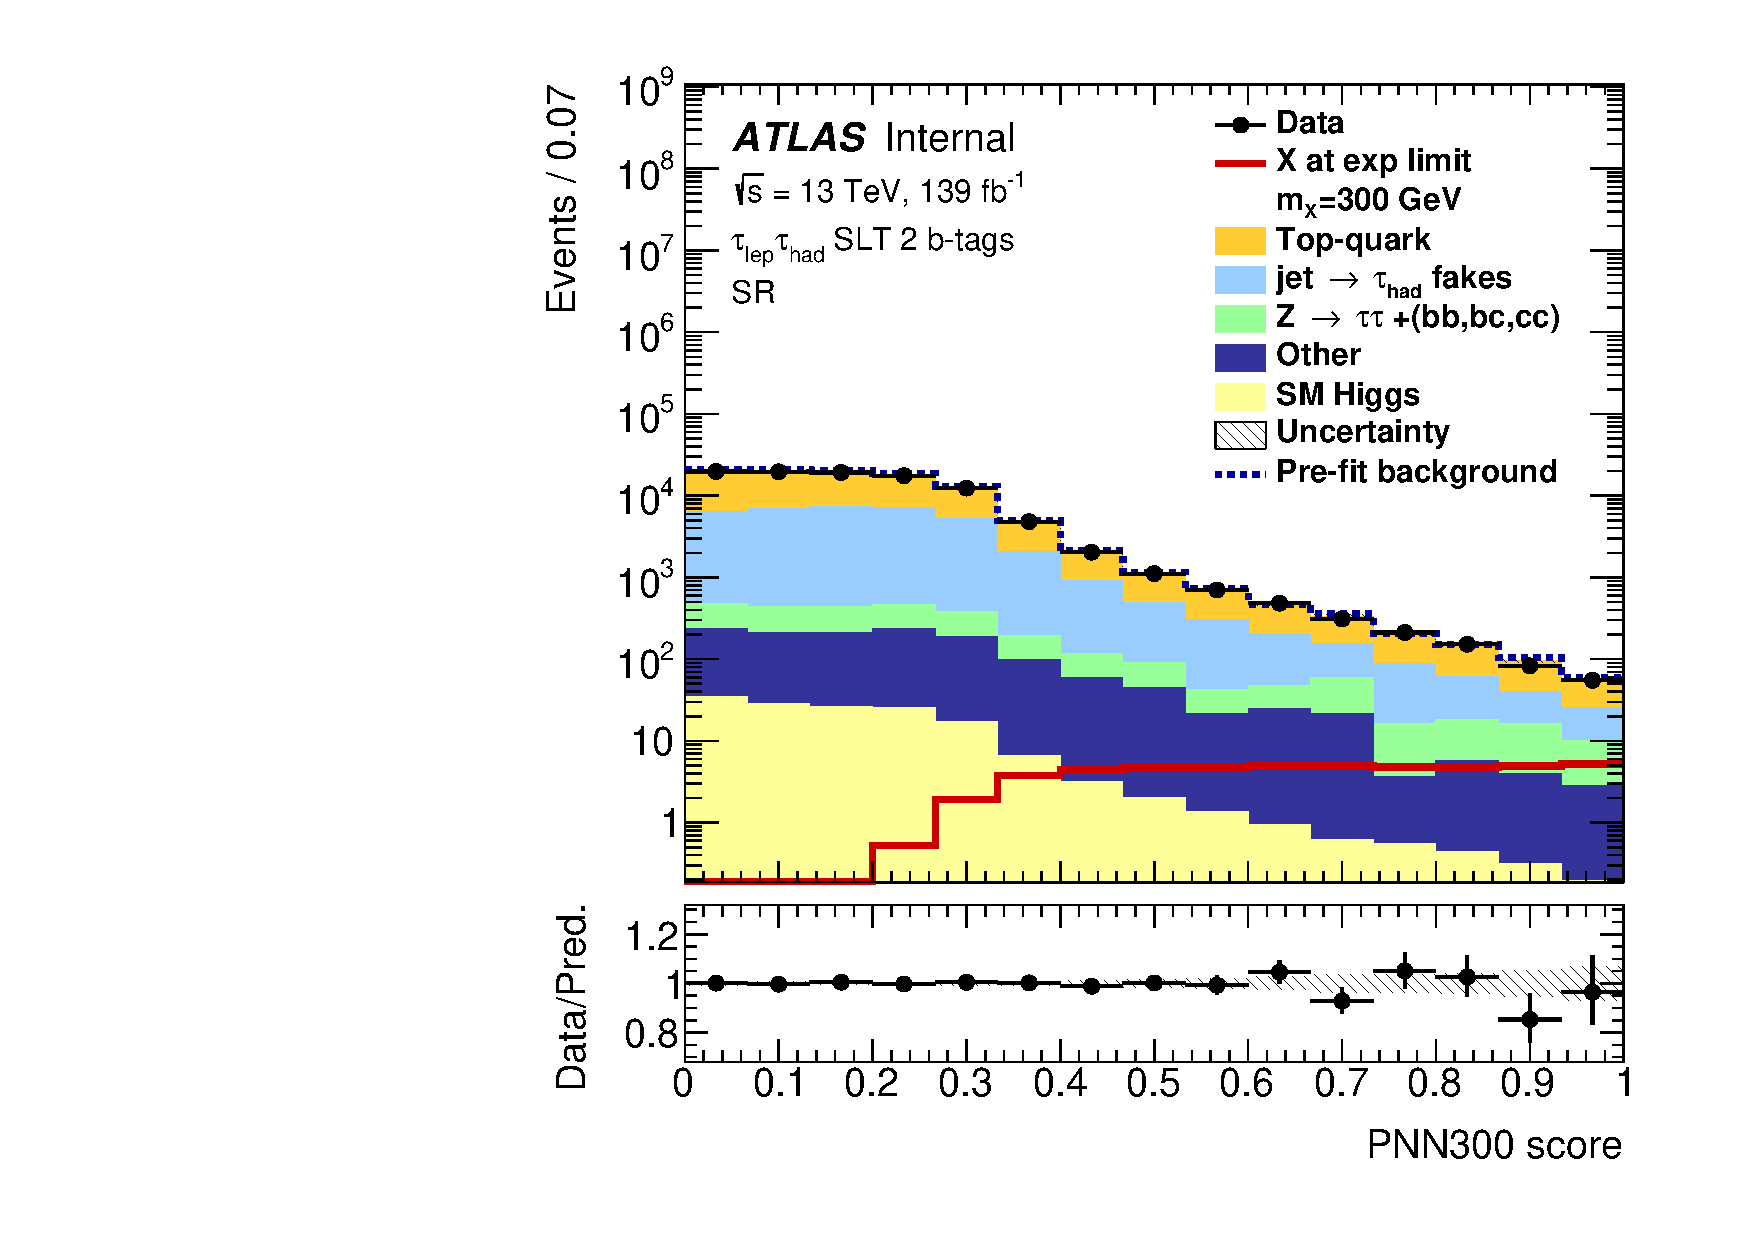
\includegraphics[width=.45\textwidth]{diHiggs/plots/MVA/postfit/Region_BMin0_incJet1_dist300_J2_D2HDMPNN_T2_SpcTauLH_Y2015_LTT0_L1_GlobalFit_conditionnal_mu0log.pdf}}\quad
% \subfloat[]
%    {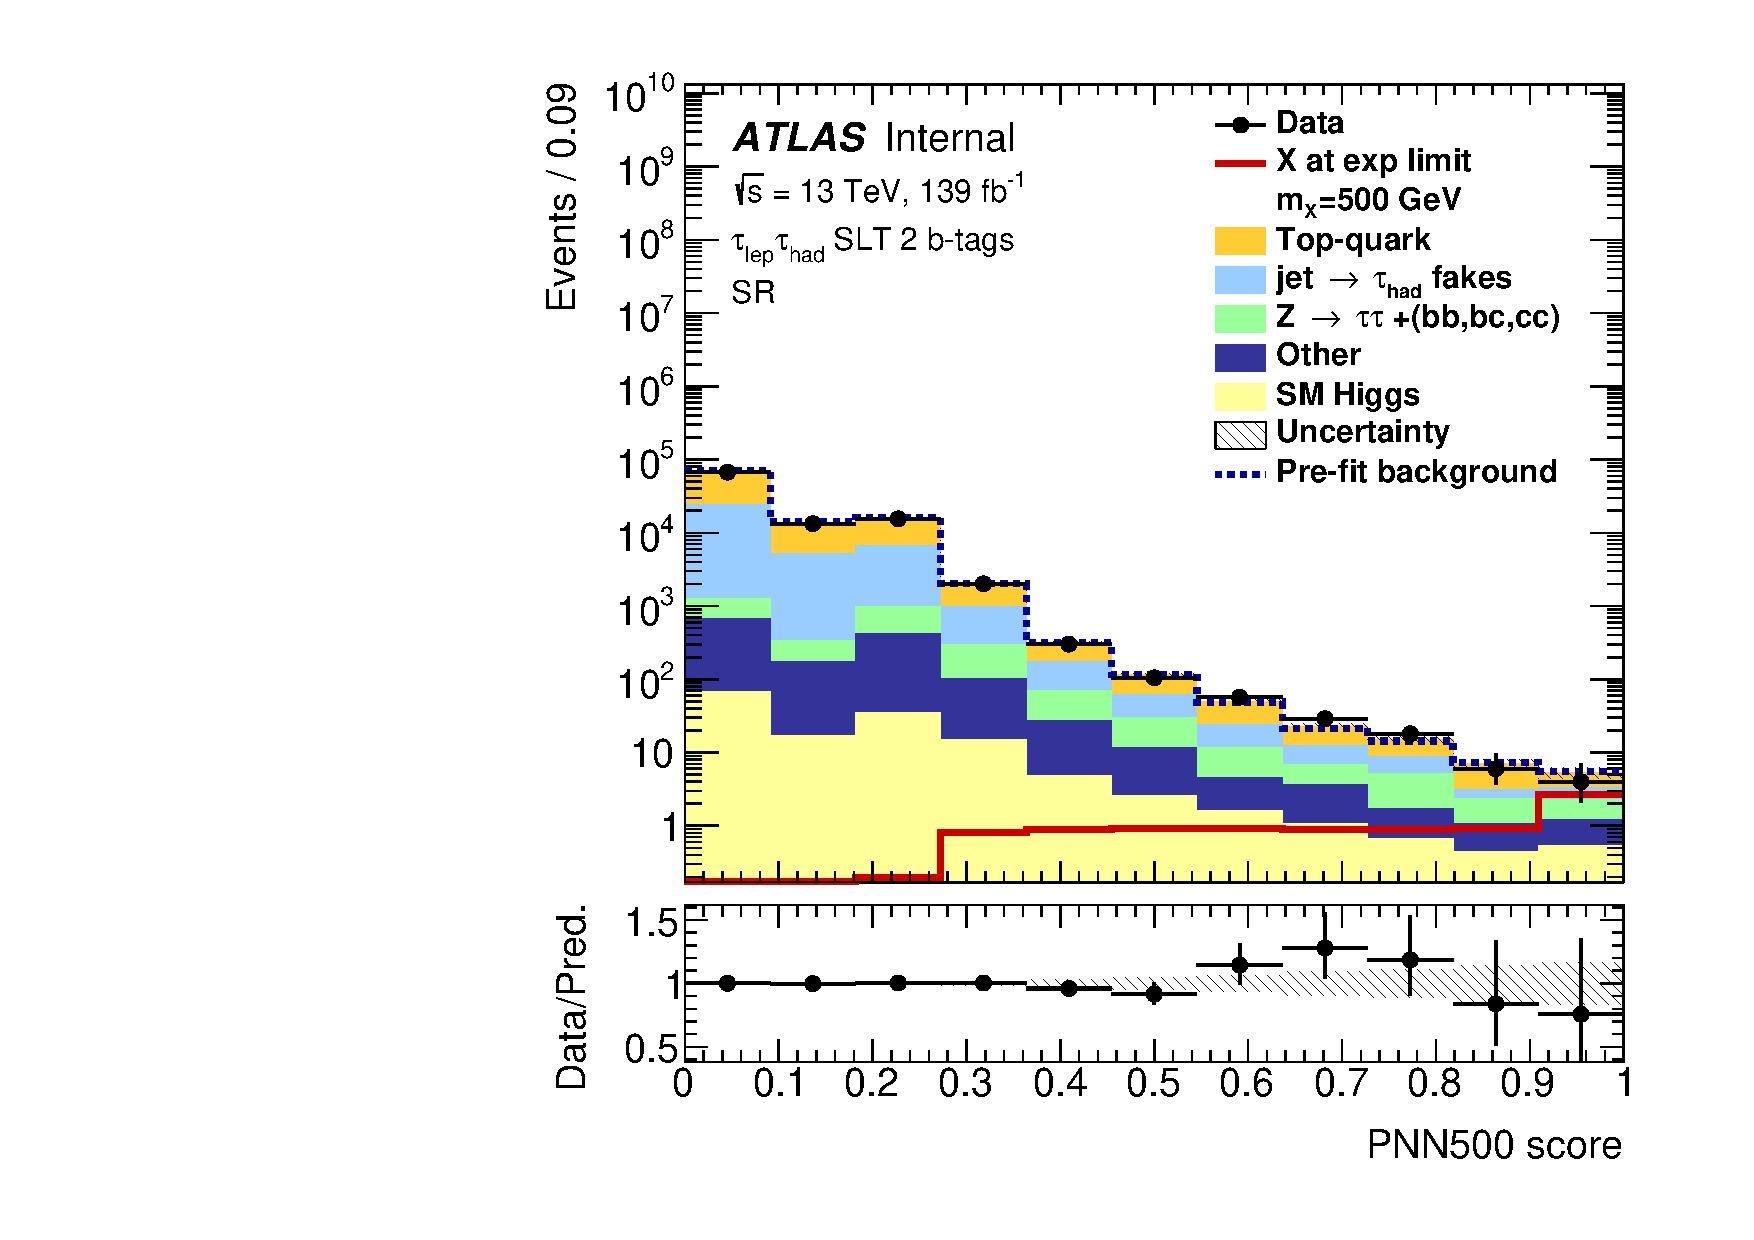
\includegraphics[width=.45\textwidth]{diHiggs/plots/MVA/postfit/Region_BMin0_incJet1_dist500_J2_D2HDMPNN_T2_SpcTauLH_Y2015_LTT0_L1_GlobalFit_conditionnal_mu0log.pdf}} \quad
% \subfloat[]
%    {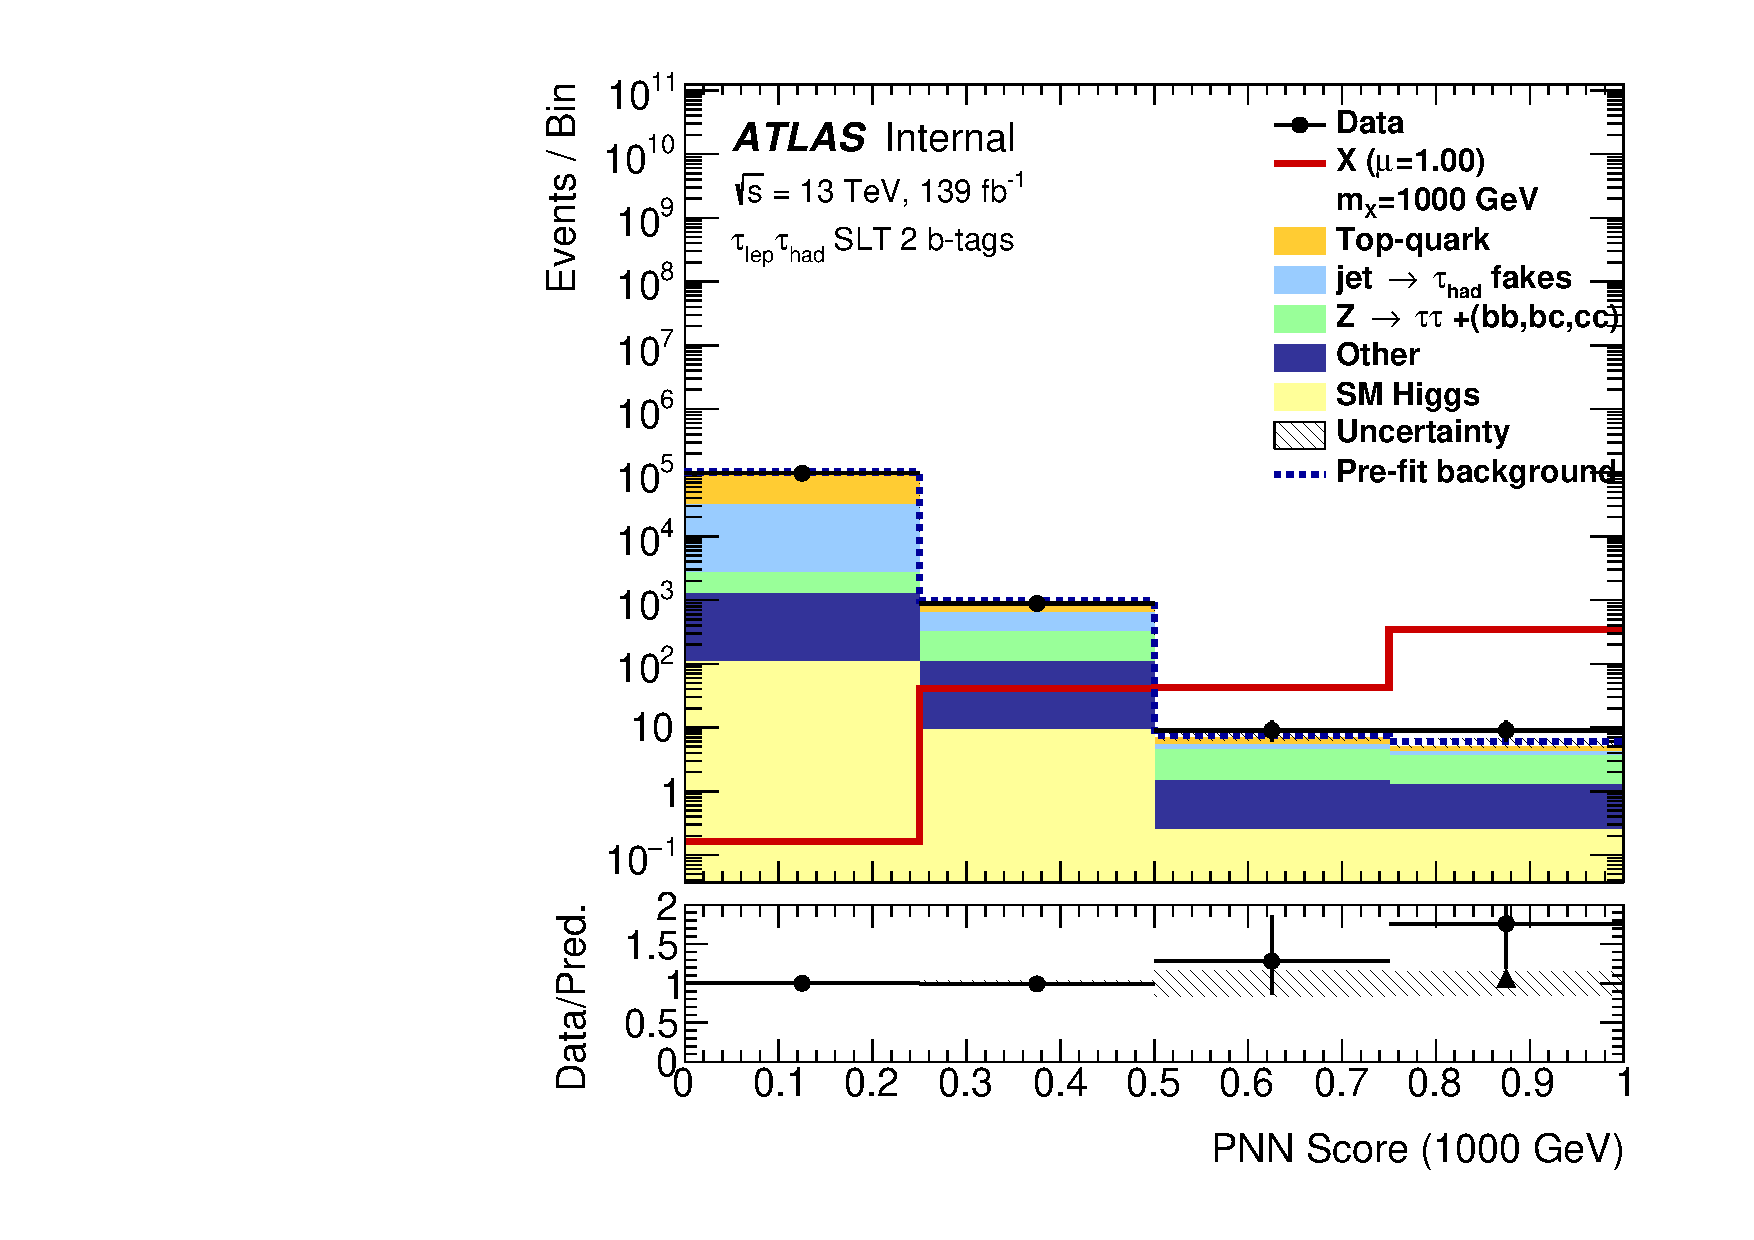
\includegraphics[width=.45\textwidth]{diHiggs/plots/MVA/postfit/Region_BMin0_incJet1_dist1000_J2_D2HDMPNN_T2_SpcTauLH_Y2015_LTT0_L1_GlobalFit_conditionnal_mu0log.pdf}}\quad
% \subfloat[]
%    {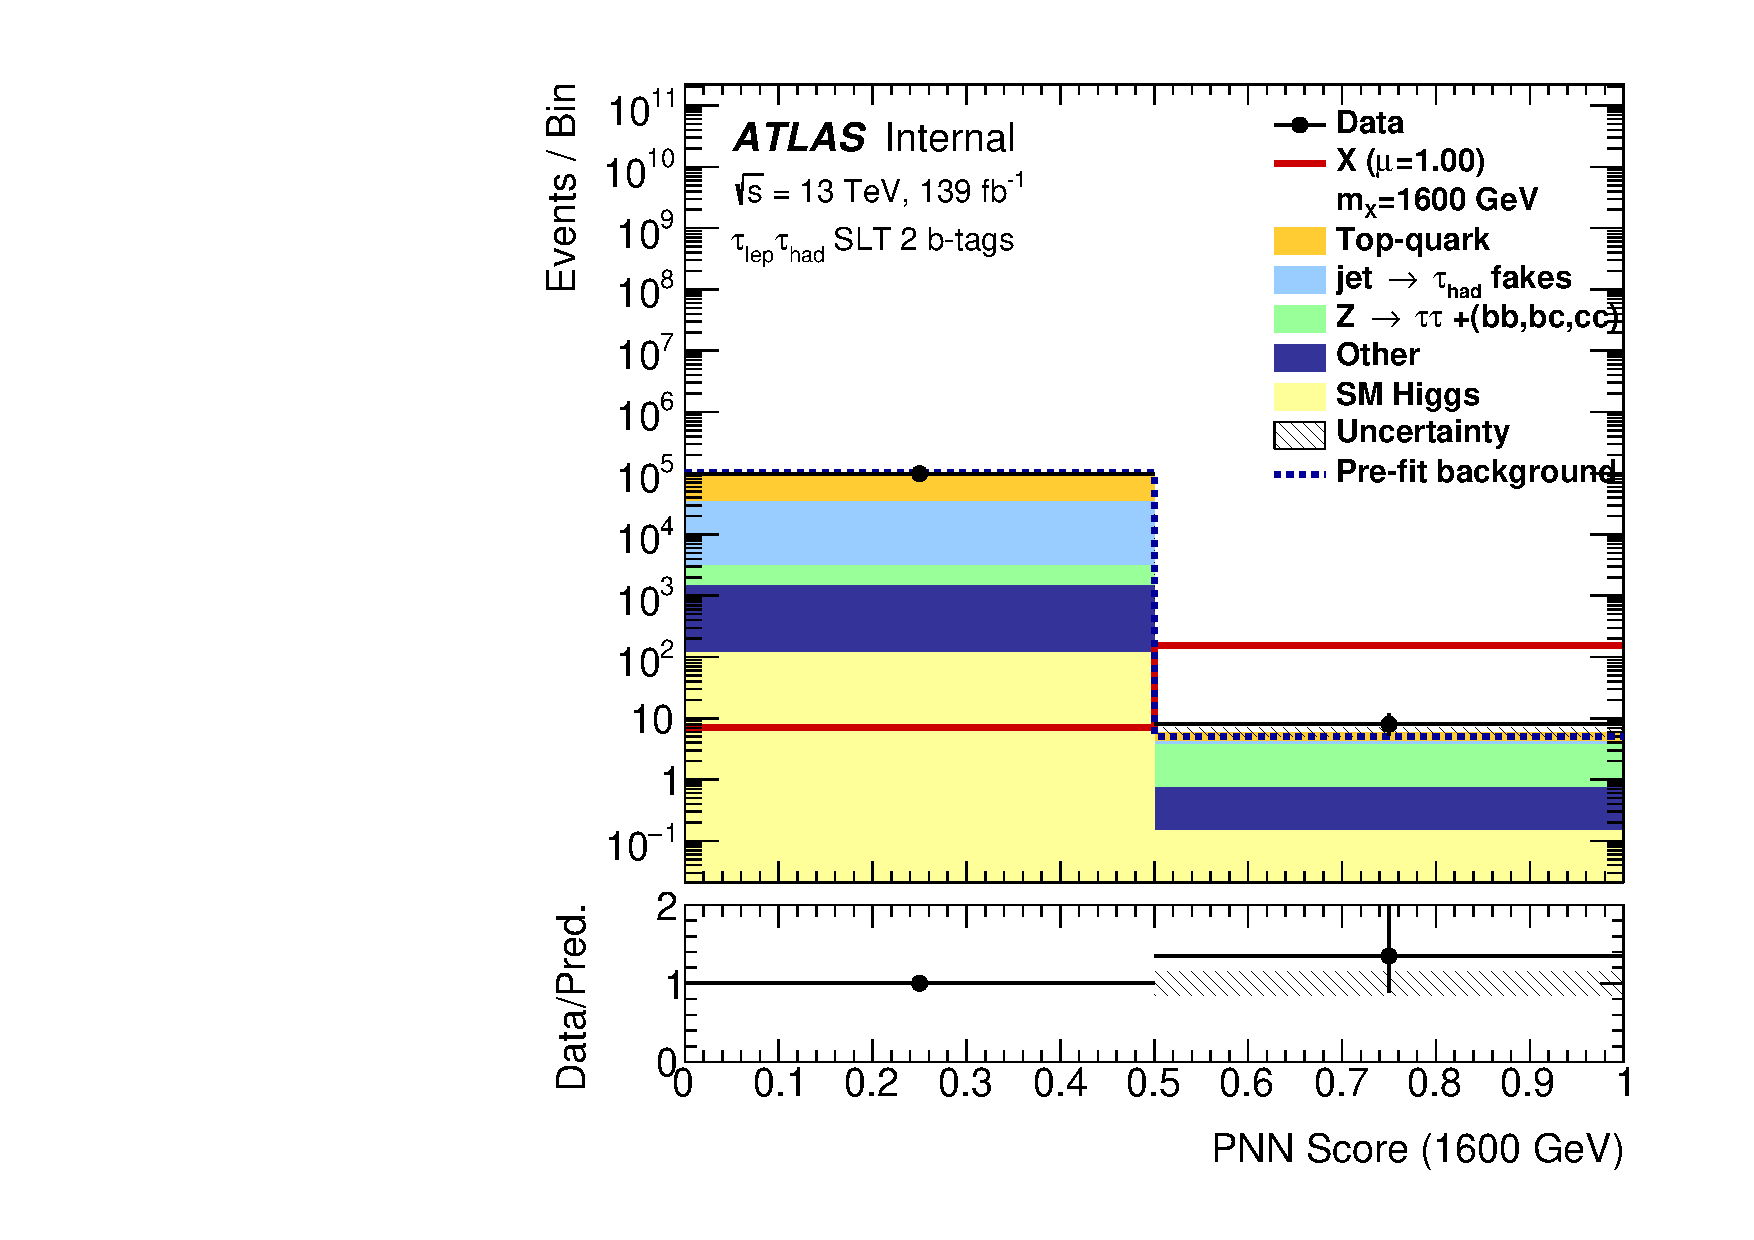
\includegraphics[width=.45\textwidth]{diHiggs/plots/MVA/postfit/Region_BMin0_incJet1_dist1600_J2_D2HDMPNN_T2_SpcTauLH_Y2015_LTT0_L1_GlobalFit_conditionnal_mu0log.pdf}}\quad
% \subfloat[]
%    {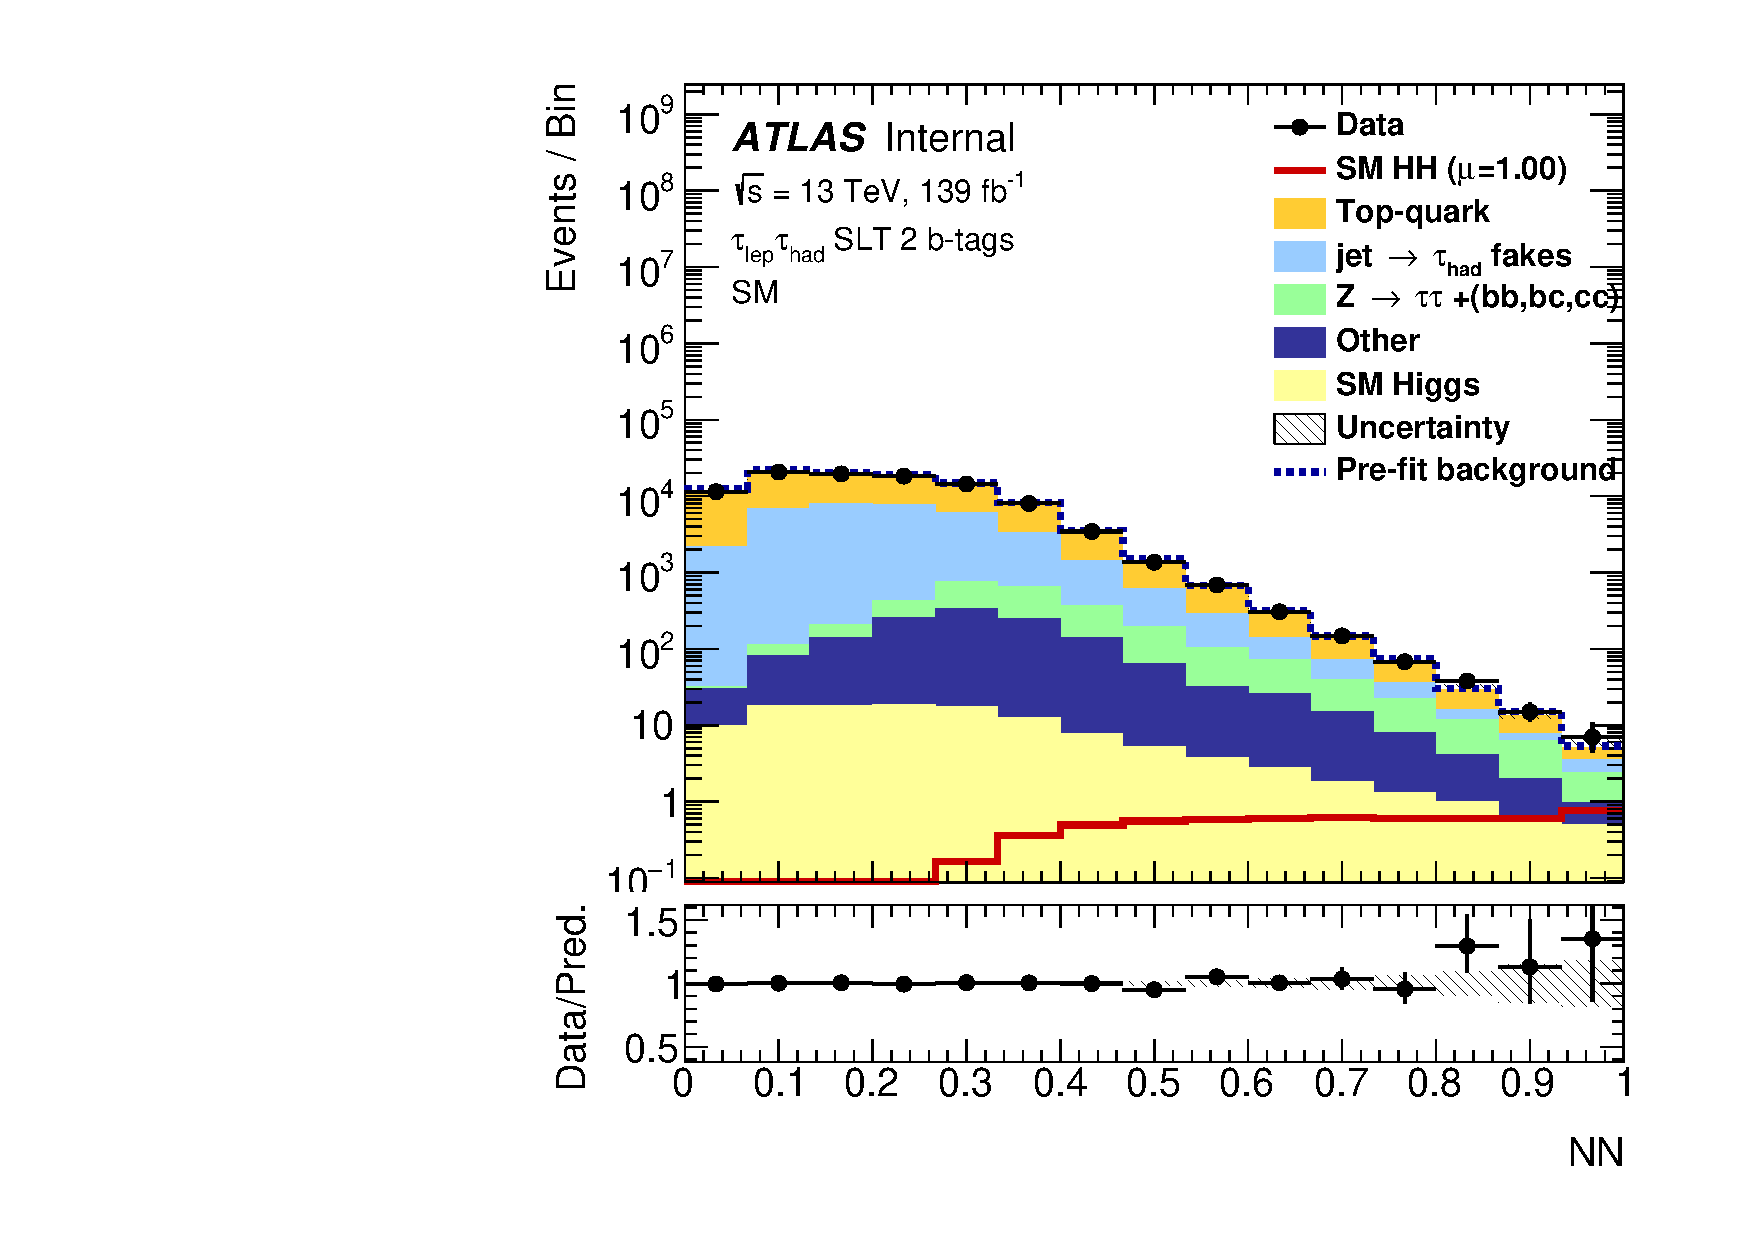
\includegraphics[width=.45\textwidth]{diHiggs/plots/MVA/postfit/Region_BMin0_incJet1_distNN_J2_DSM_T2_SpcTauLH_Y2015_LTT0_L1_GlobalFit_conditionnal_mu0log.pdf}}\quad
% \caption{Post-fit PNN score distributions for the $300, 500, 1000, 1600$ GeV mass points and post-fit SM NN distribution in the di-Higgs $bb\lephad$ SLT signal region from the \lephad background-only fit. The uncertainty band includes the systematic uncertainties.}
% \label{fig:LepHadSLTPostfitPNNScoreDistributions}
% \end{figure}

% \begin{figure}[htbp]
% \centering
% \subfloat[]
%    {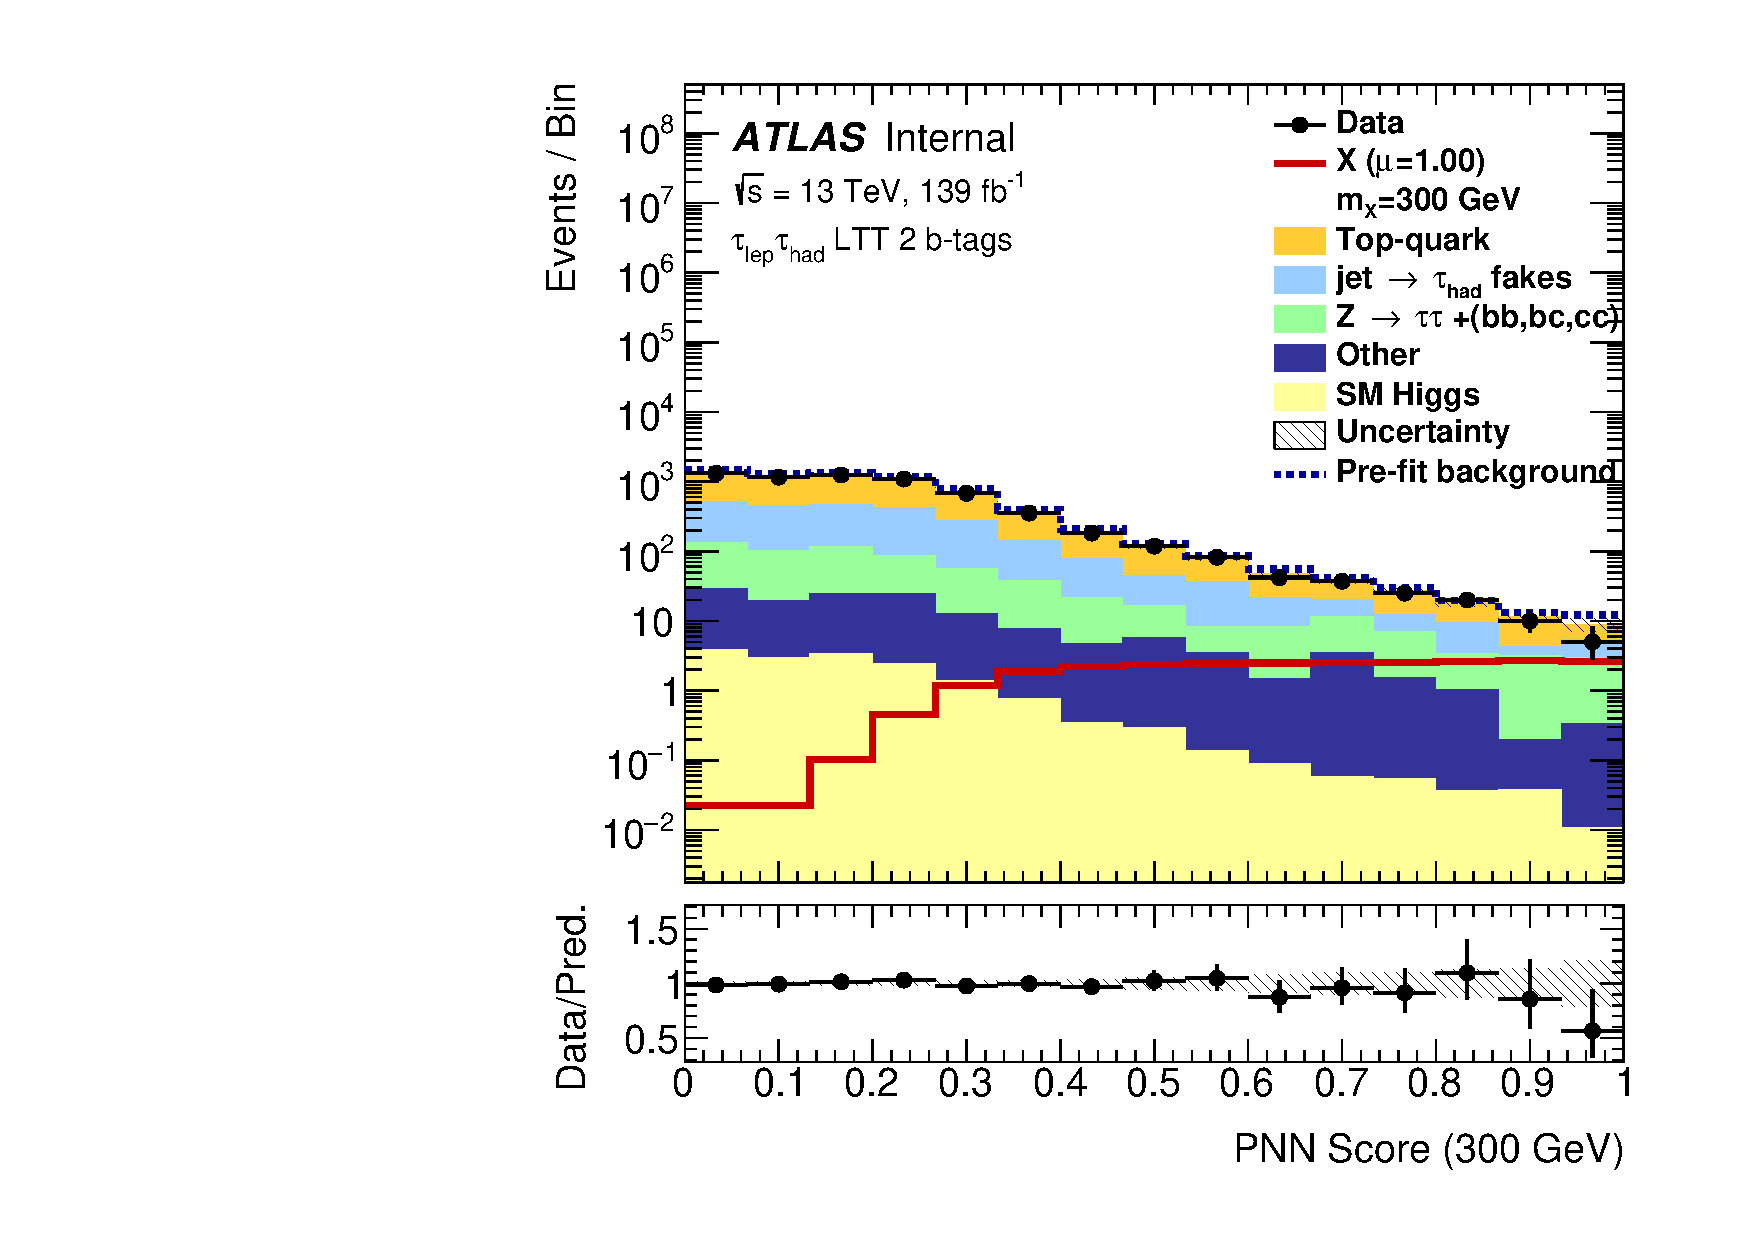
\includegraphics[width=.45\textwidth]{diHiggs/plots/MVA/postfit/Region_BMin0_incJet1_dist300_J2_D2HDMPNN_T2_SpcTauLH_Y2015_LTT1_L1_GlobalFit_conditionnal_mu0log.pdf}}\quad
% \subfloat[]
%    {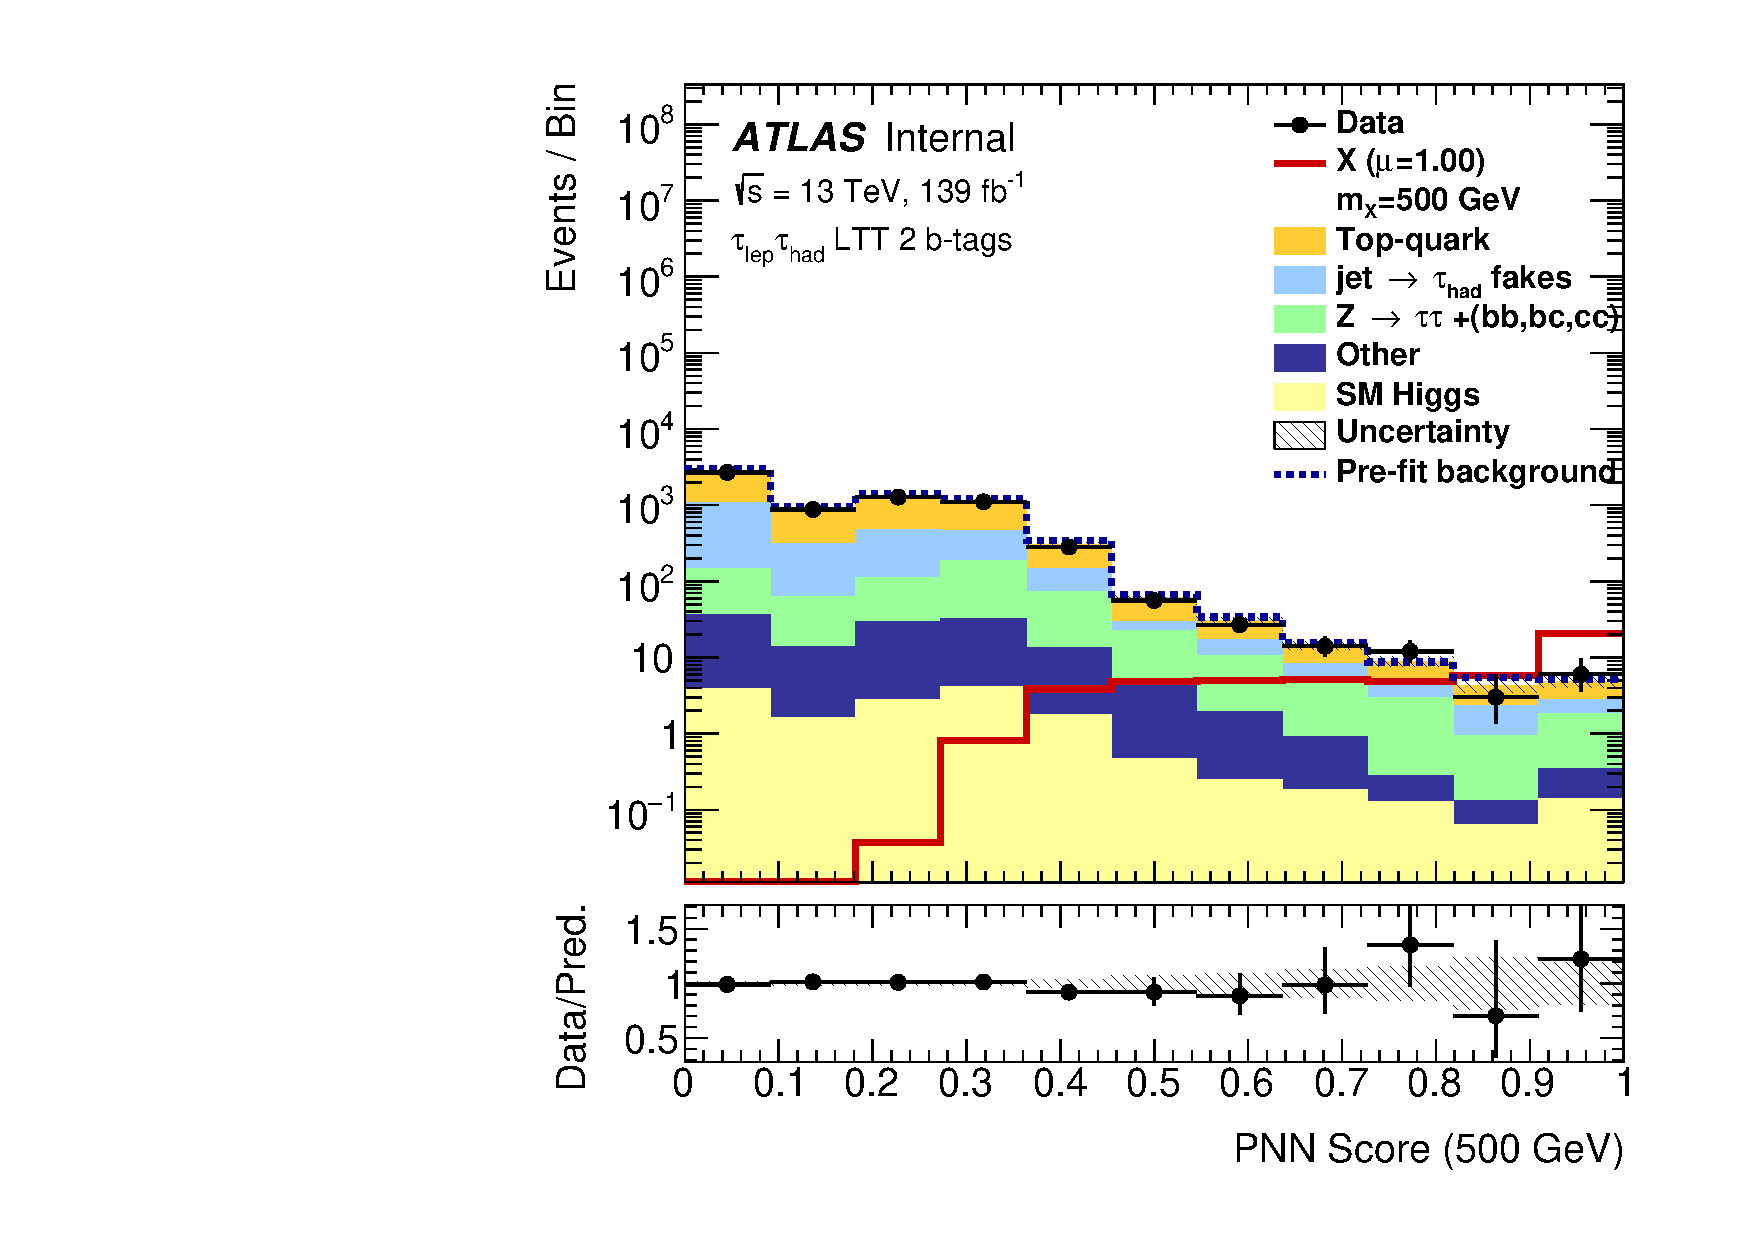
\includegraphics[width=.45\textwidth]{diHiggs/plots/MVA/postfit/Region_BMin0_incJet1_dist500_J2_D2HDMPNN_T2_SpcTauLH_Y2015_LTT1_L1_GlobalFit_conditionnal_mu0log.pdf}} \quad
% \subfloat[]
%    {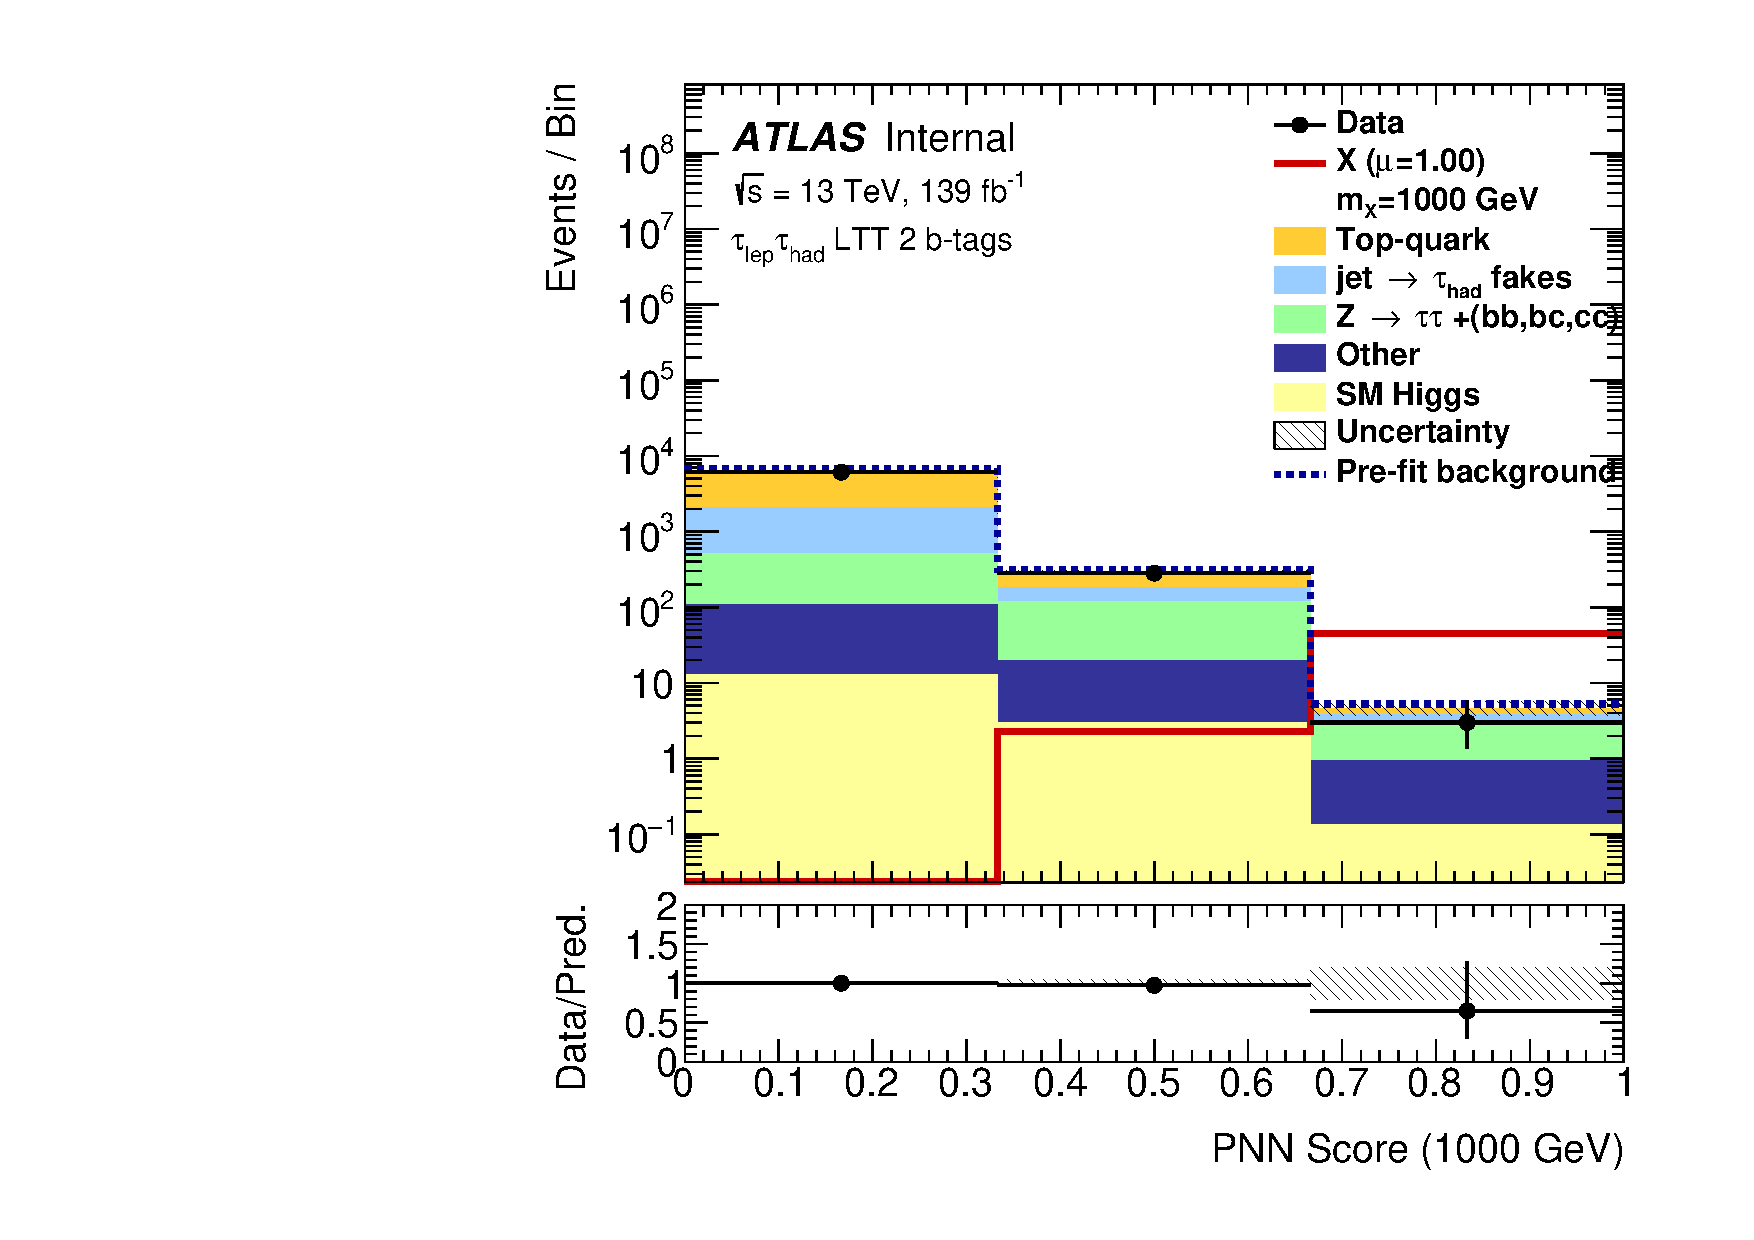
\includegraphics[width=.45\textwidth]{diHiggs/plots/MVA/postfit/Region_BMin0_incJet1_dist1000_J2_D2HDMPNN_T2_SpcTauLH_Y2015_LTT1_L1_GlobalFit_conditionnal_mu0log.pdf}}\quad
% \subfloat[]
%    {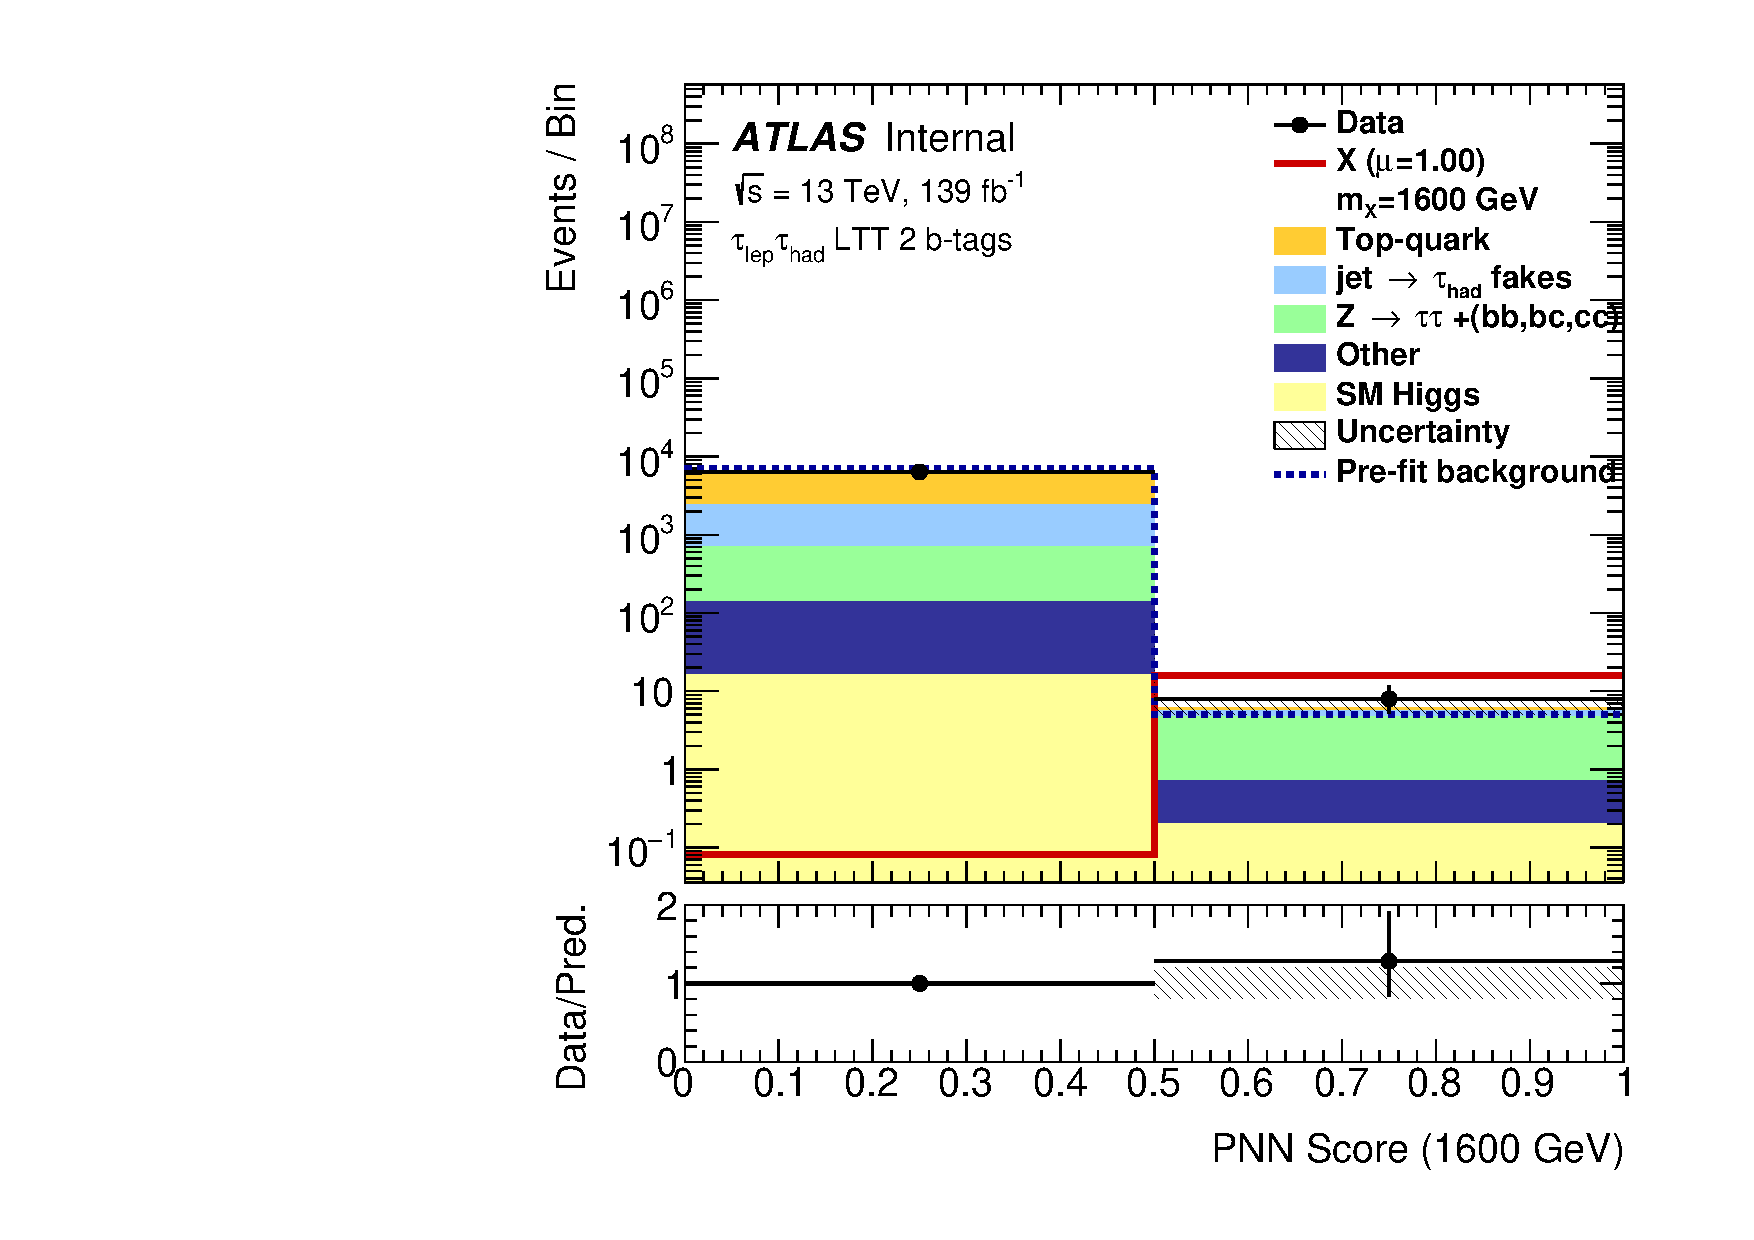
\includegraphics[width=.45\textwidth]{diHiggs/plots/MVA/postfit/Region_BMin0_incJet1_dist1600_J2_D2HDMPNN_T2_SpcTauLH_Y2015_LTT1_L1_GlobalFit_conditionnal_mu0log.pdf}}\quad
% \subfloat[]
%    {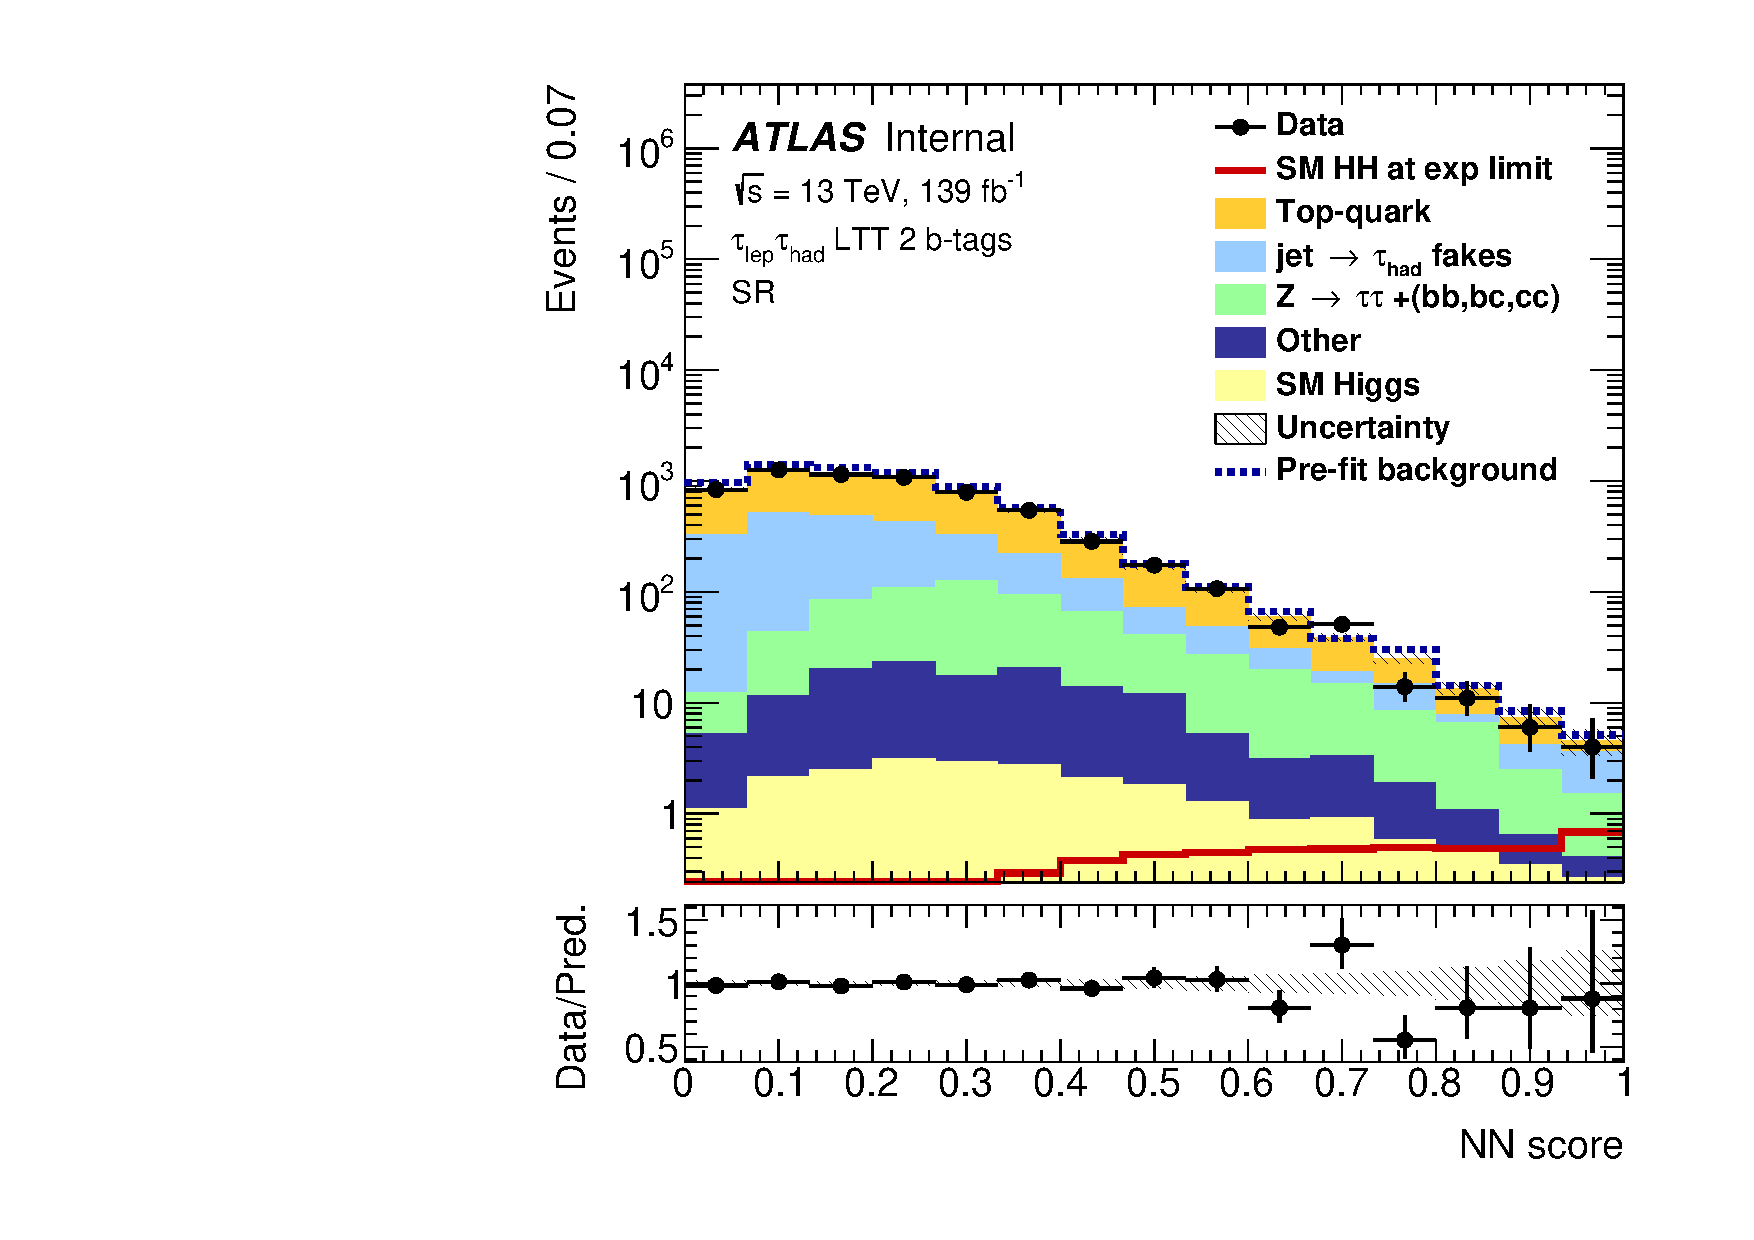
\includegraphics[width=.45\textwidth]{diHiggs/plots/MVA/postfit/Region_BMin0_incJet1_distNN_J2_DSM_T2_SpcTauLH_Y2015_LTT1_L1_GlobalFit_conditionnal_mu0log.pdf}}\quad
% \caption{Post-fit PNN score distributions for the $300, 500, 1000, 1600$ GeV mass points and post-fit SM NN distribution in the di-Higgs $bb\lephad$ LTT signal region from the \lephad background-only fit. The uncertainty band includes the systematic uncertainties.}
% \label{fig:LepHadLTTPostfitPNNScoreDistributions}
% \end{figure}
\begin{figure}
\centering
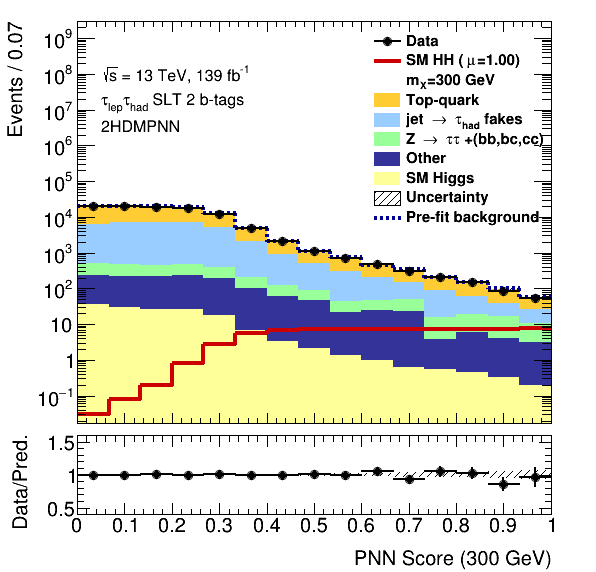
\includegraphics[width=.32\textwidth]{diHiggs/plots/MVA_plots/Region_BMin0_incJet1_dist300_J2_D2HDMPNN_T2_SpcTauLH_Y2015_LTT0_L1_GlobalFit_conditionnal_mu0log.png}
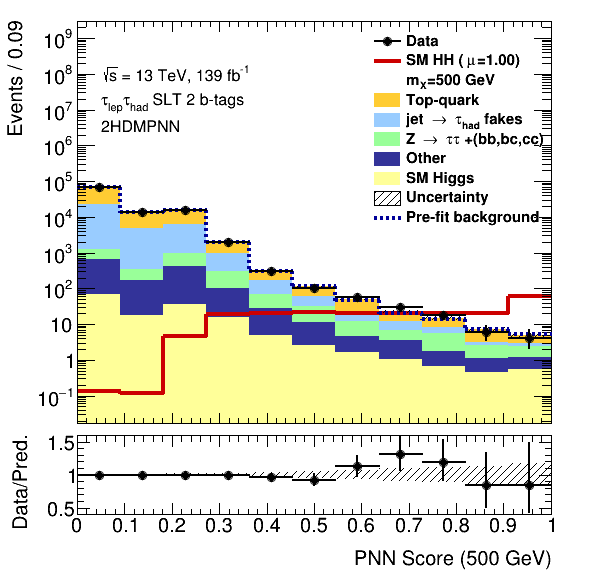
\includegraphics[width=.32\textwidth]{diHiggs/plots/MVA_plots/Region_BMin0_incJet1_dist500_J2_D2HDMPNN_T2_SpcTauLH_Y2015_LTT0_L1_GlobalFit_conditionnal_mu0log.png}
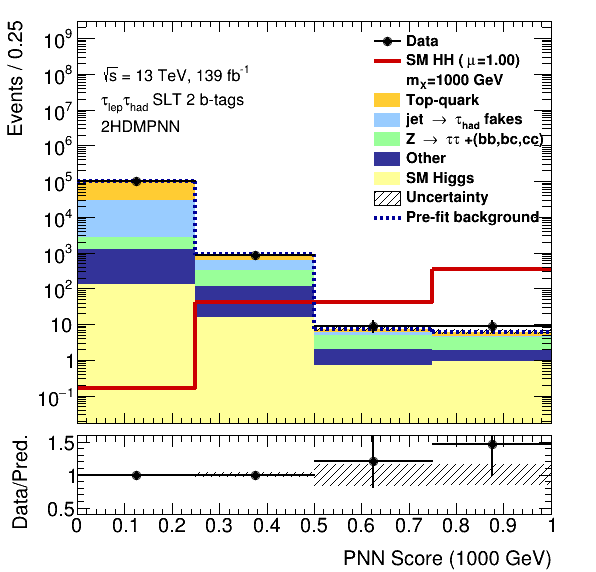
\includegraphics[width=.32\textwidth]{diHiggs/plots/MVA_plots/Region_BMin0_incJet1_dist1000_J2_D2HDMPNN_T2_SpcTauLH_Y2015_LTT0_L1_GlobalFit_conditionnal_mu0log.png} \\
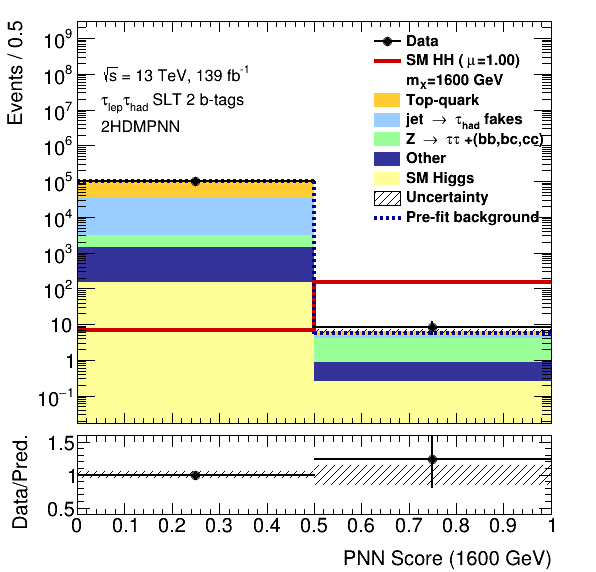
\includegraphics[width=.32\textwidth]{diHiggs/plots/MVA_plots/Region_BMin0_incJet1_dist1600_J2_D2HDMPNN_T2_SpcTauLH_Y2015_LTT0_L1_GlobalFit_conditionnal_mu0log.png} 
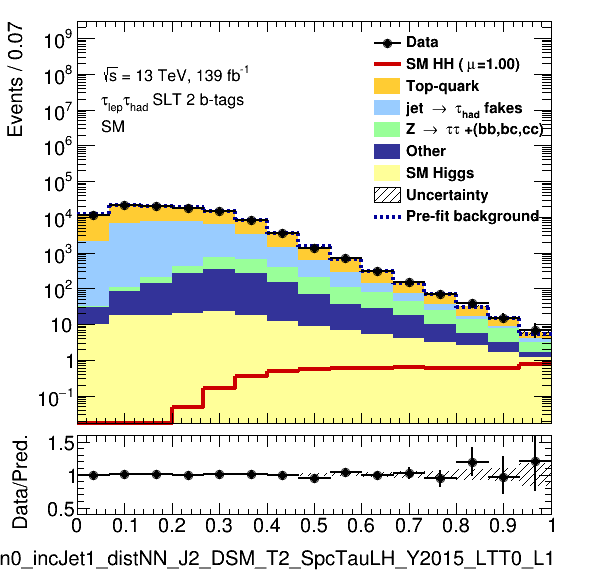
\includegraphics[width=.32\textwidth]{diHiggs/plots/MVA_plots/Region_BMin0_incJet1_distNN_J2_DSM_T2_SpcTauLH_Y2015_LTT0_L1_GlobalFit_conditionnal_mu0log.png} \\
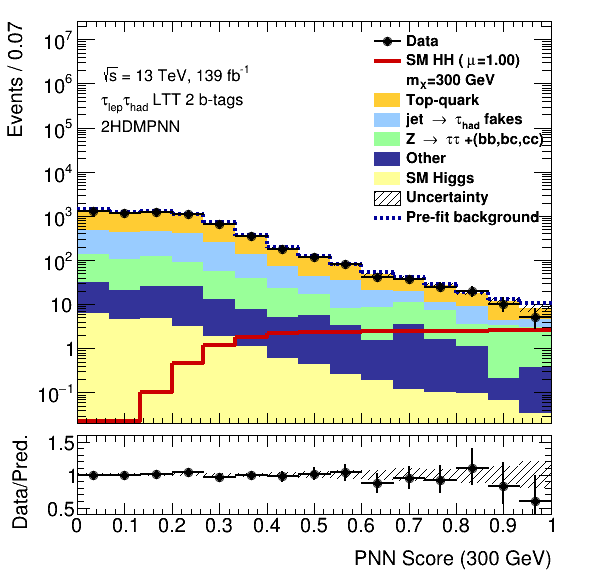
\includegraphics[width=.32\textwidth]{diHiggs/plots/MVA_plots/Region_BMin0_incJet1_dist300_J2_D2HDMPNN_T2_SpcTauLH_Y2015_LTT1_L1_GlobalFit_conditionnal_mu0log.png}
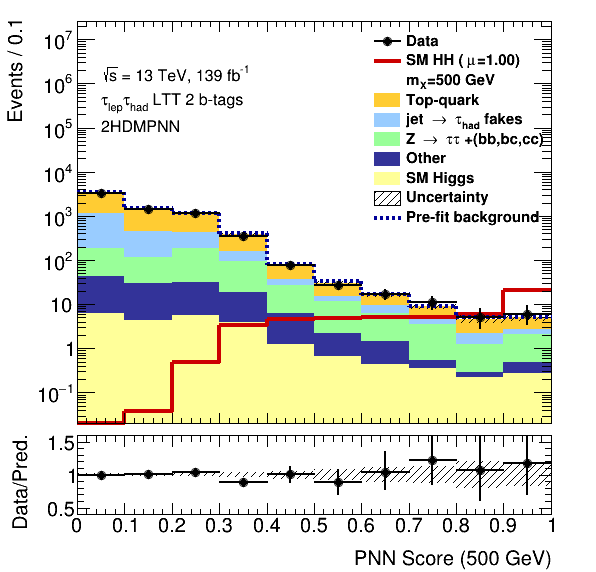
\includegraphics[width=.32\textwidth]{diHiggs/plots/MVA_plots/Region_BMin0_incJet1_dist500_J2_D2HDMPNN_T2_SpcTauLH_Y2015_LTT1_L1_GlobalFit_conditionnal_mu0log.png}
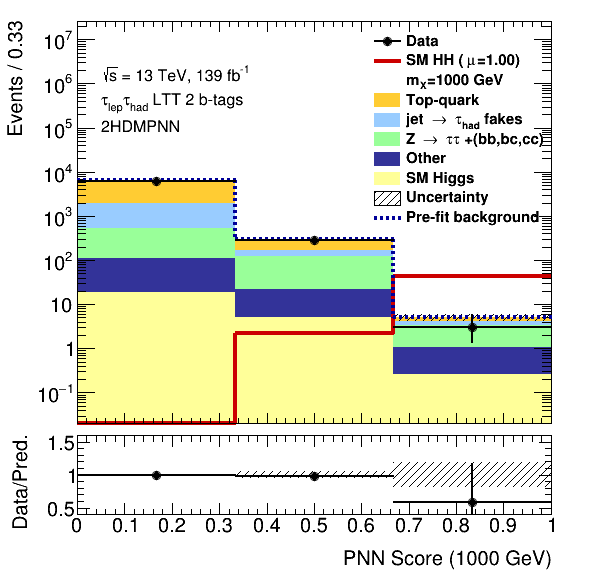
\includegraphics[width=.32\textwidth]{diHiggs/plots/MVA_plots/Region_BMin0_incJet1_dist1000_J2_D2HDMPNN_T2_SpcTauLH_Y2015_LTT1_L1_GlobalFit_conditionnal_mu0log.png} \\
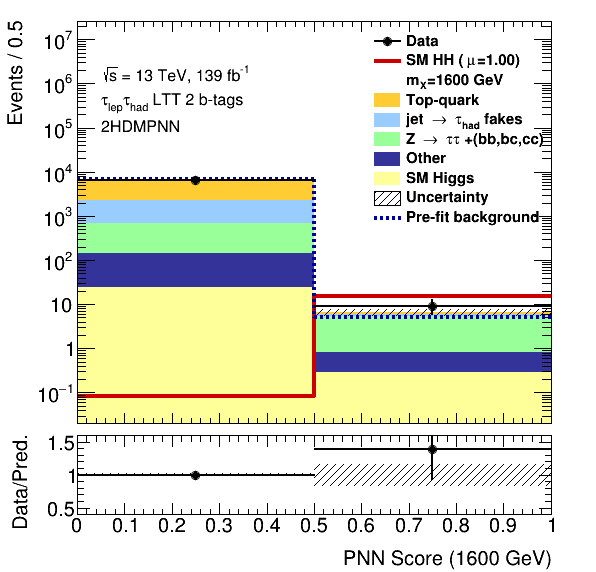
\includegraphics[width=.32\textwidth]{diHiggs/plots/MVA_plots/Region_BMin0_incJet1_dist1600_J2_D2HDMPNN_T2_SpcTauLH_Y2015_LTT1_L1_GlobalFit_conditionnal_mu0log.png} 
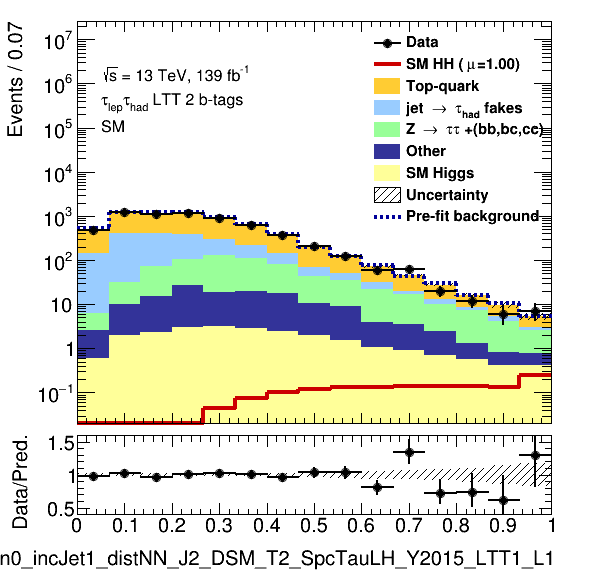
\includegraphics[width=.32\textwidth]{diHiggs/plots/MVA_plots/Region_BMin0_incJet1_distNN_J2_DSM_T2_SpcTauLH_Y2015_LTT1_L1_GlobalFit_conditionnal_mu0log.png}
\caption{Post-fit PNN score distributions for the $300, 500, 1000, 1600$ GeV mass points and 
non-resonant NN in the di-Higgs $bb\lephad$ SLT (top two rows) and LTT (bottom two rows) signal regions.}
\label{fig:LepHadPostfitPNNScoreDistributions}
\end{figure}
    


The non-resonant $HH$ signal with \kl\ values are passed to the same NN classification used
for the SM $HH$ signal. The NN score of non-resonant $HH$ with \kl\ = -5, -3, -1.6, 1, 2, 7 and 10 
samples are shown in Figure~\ref{fig:postfit_slt} (\ref{fig:postfit_ltt}) for the SLT (LTT) channel.
As the NN has only been trained with SM signal,
it is expected that the separation power will degrade for samples with \kl\ 
deviating far from 1.

% A slight underestimation of the data by the background-only expectation is found in the 
% final bin of the MVA score distribution in the two most sensitive \bbtautau signal regions, 
% while the data in the second- and third-highest score bins are slightly overestimated.

% Thus, at $\kappa_\lambda \approx 2$ a larger signal strength value can 
% be applied to improve the agreement in the final bin without strongly worsening the agreement in the second- and third-highest score bins.
% Therefore, the ratio between oberved and expected cross-section limits is highest around $\kappa_\lambda = 2$.

\begin{figure}[htbp]
\begin{center}
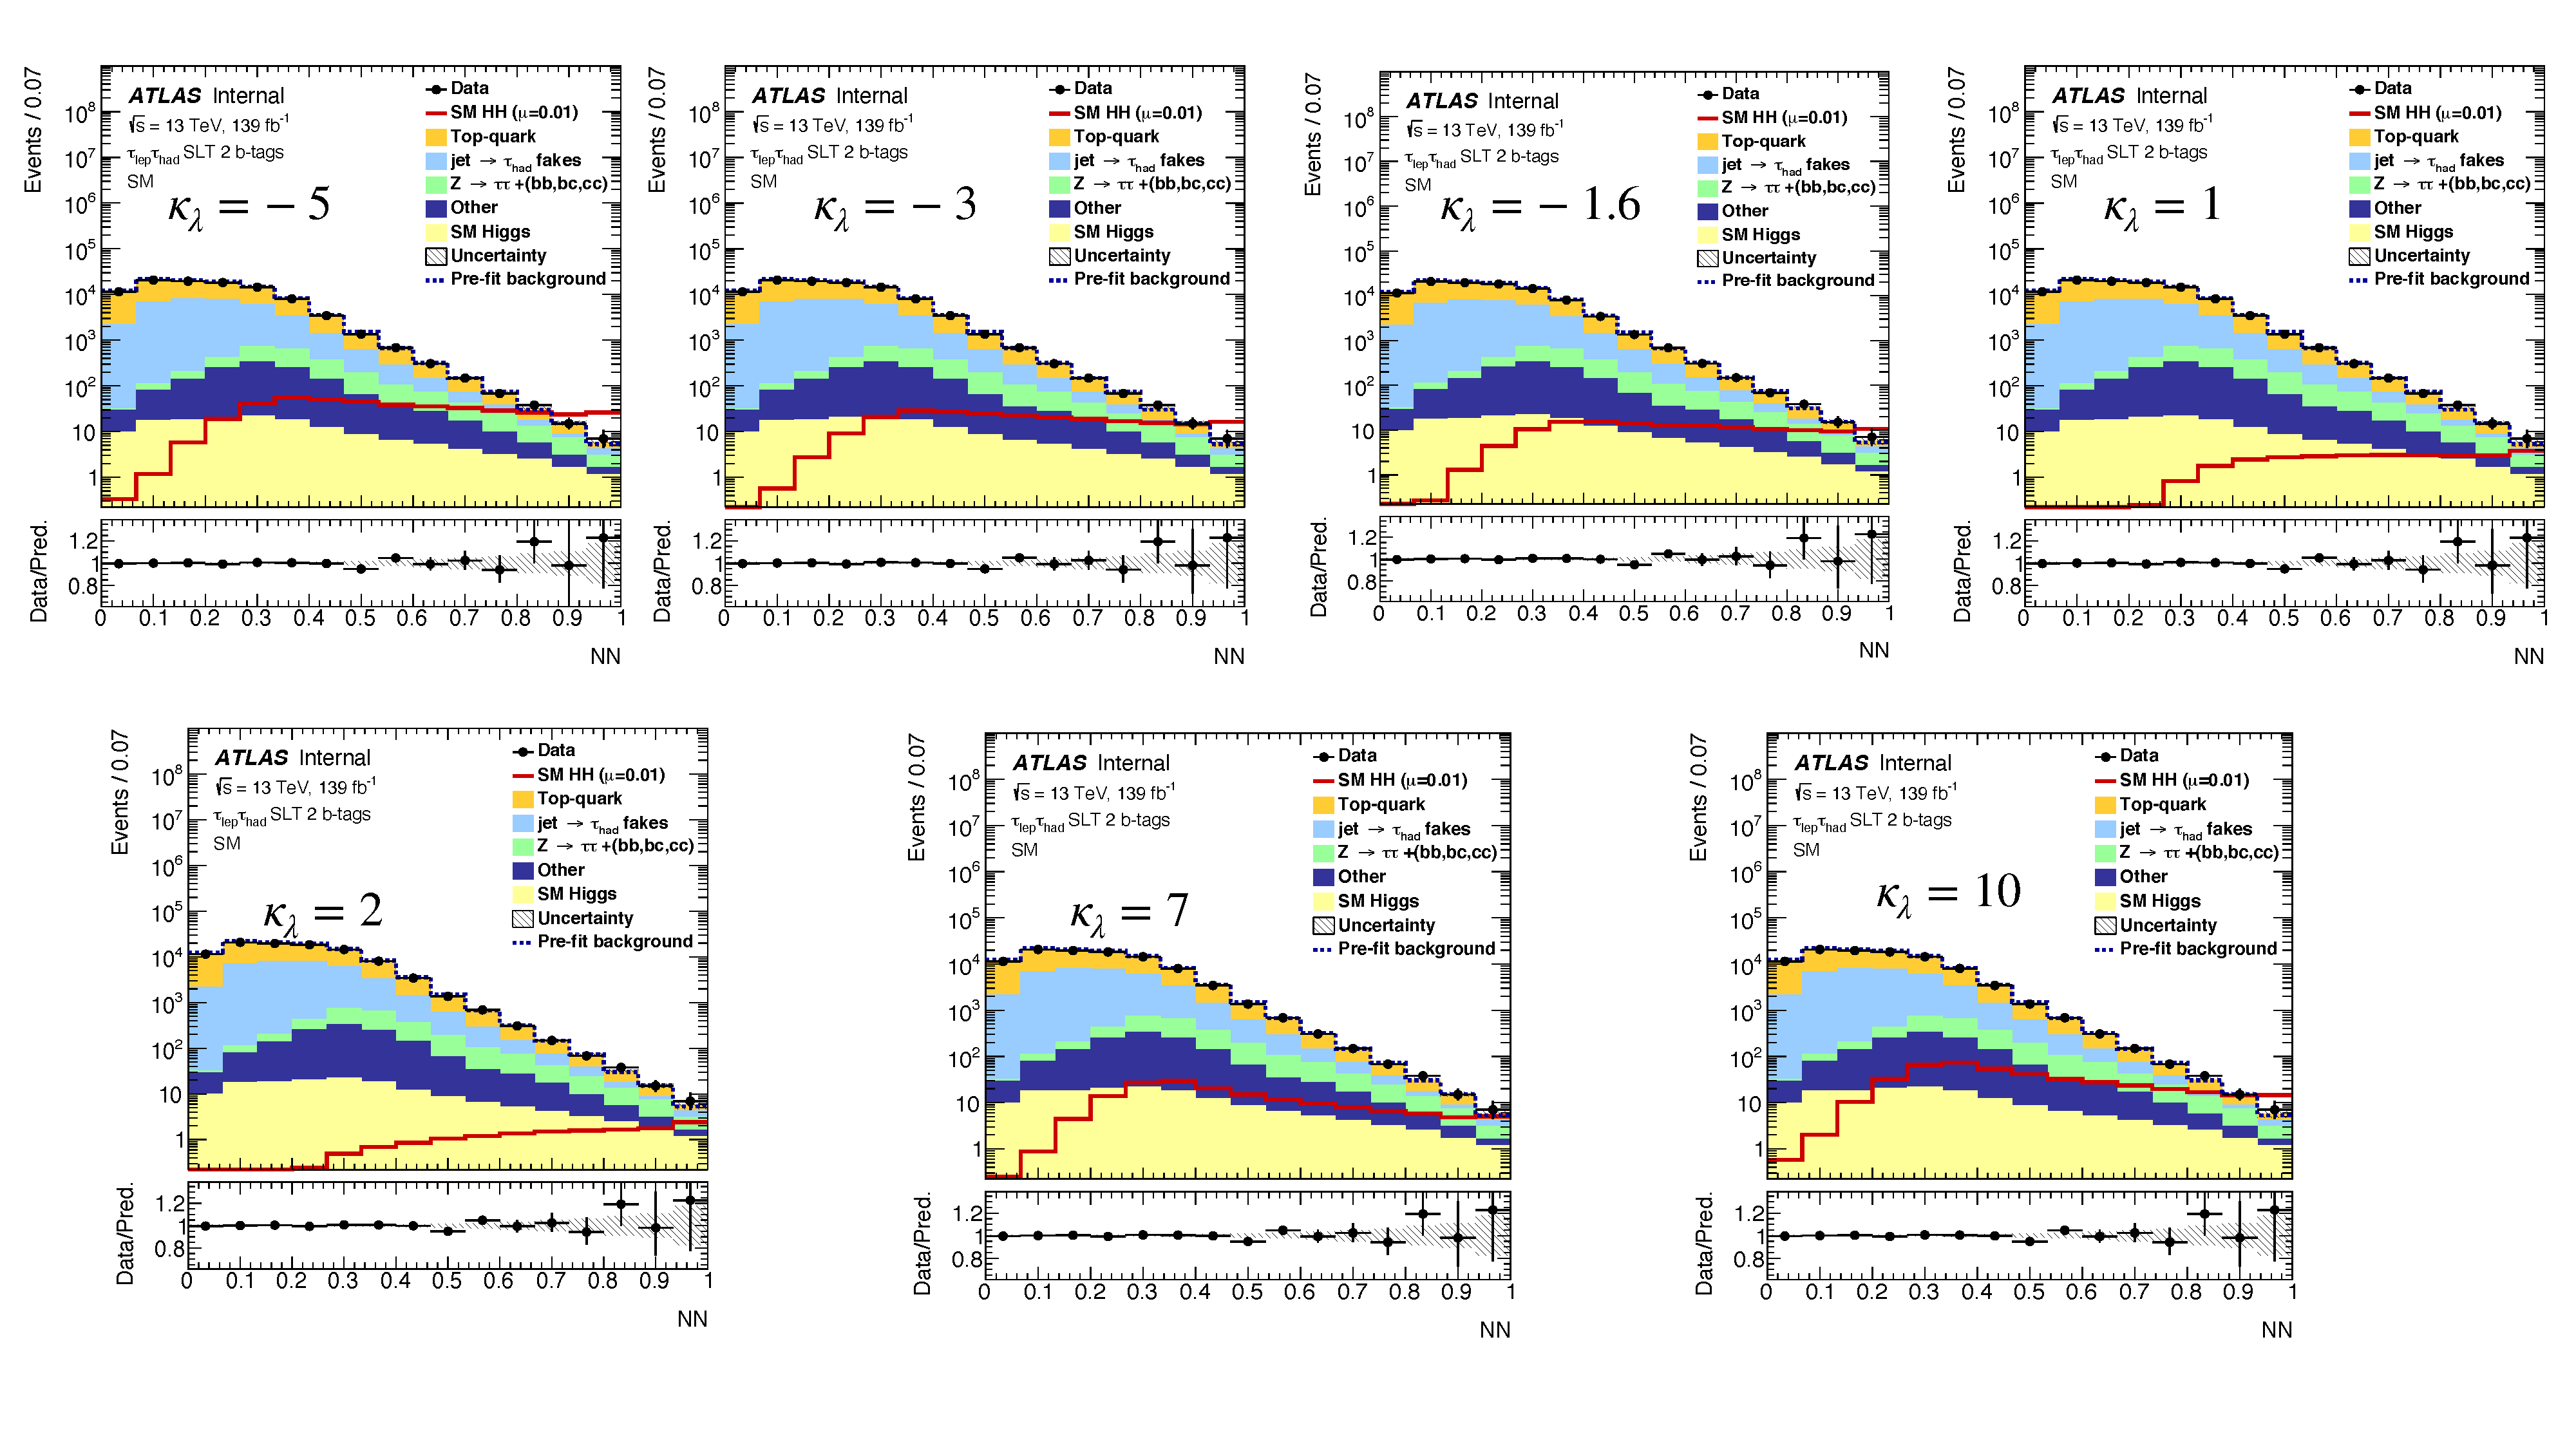
\includegraphics[width=\textwidth]{DiHiggs/plots/kl_scan/bbtautauSubchannels/bkg_only_postfit_lephad_SLT.pdf}\\
\end{center}
\caption{Post-fit plots of the neural network output in the $\tau_{\text{lep}}\tau_{\text{had}}$ SLT signal region,
showing the agreement of the background-only hypthesis with the data as well as the signal prediction for different $\kappa_\lambda$ values.}
\label{fig:postfit_slt}
\end{figure}

\begin{figure}[htbp]
\begin{center}
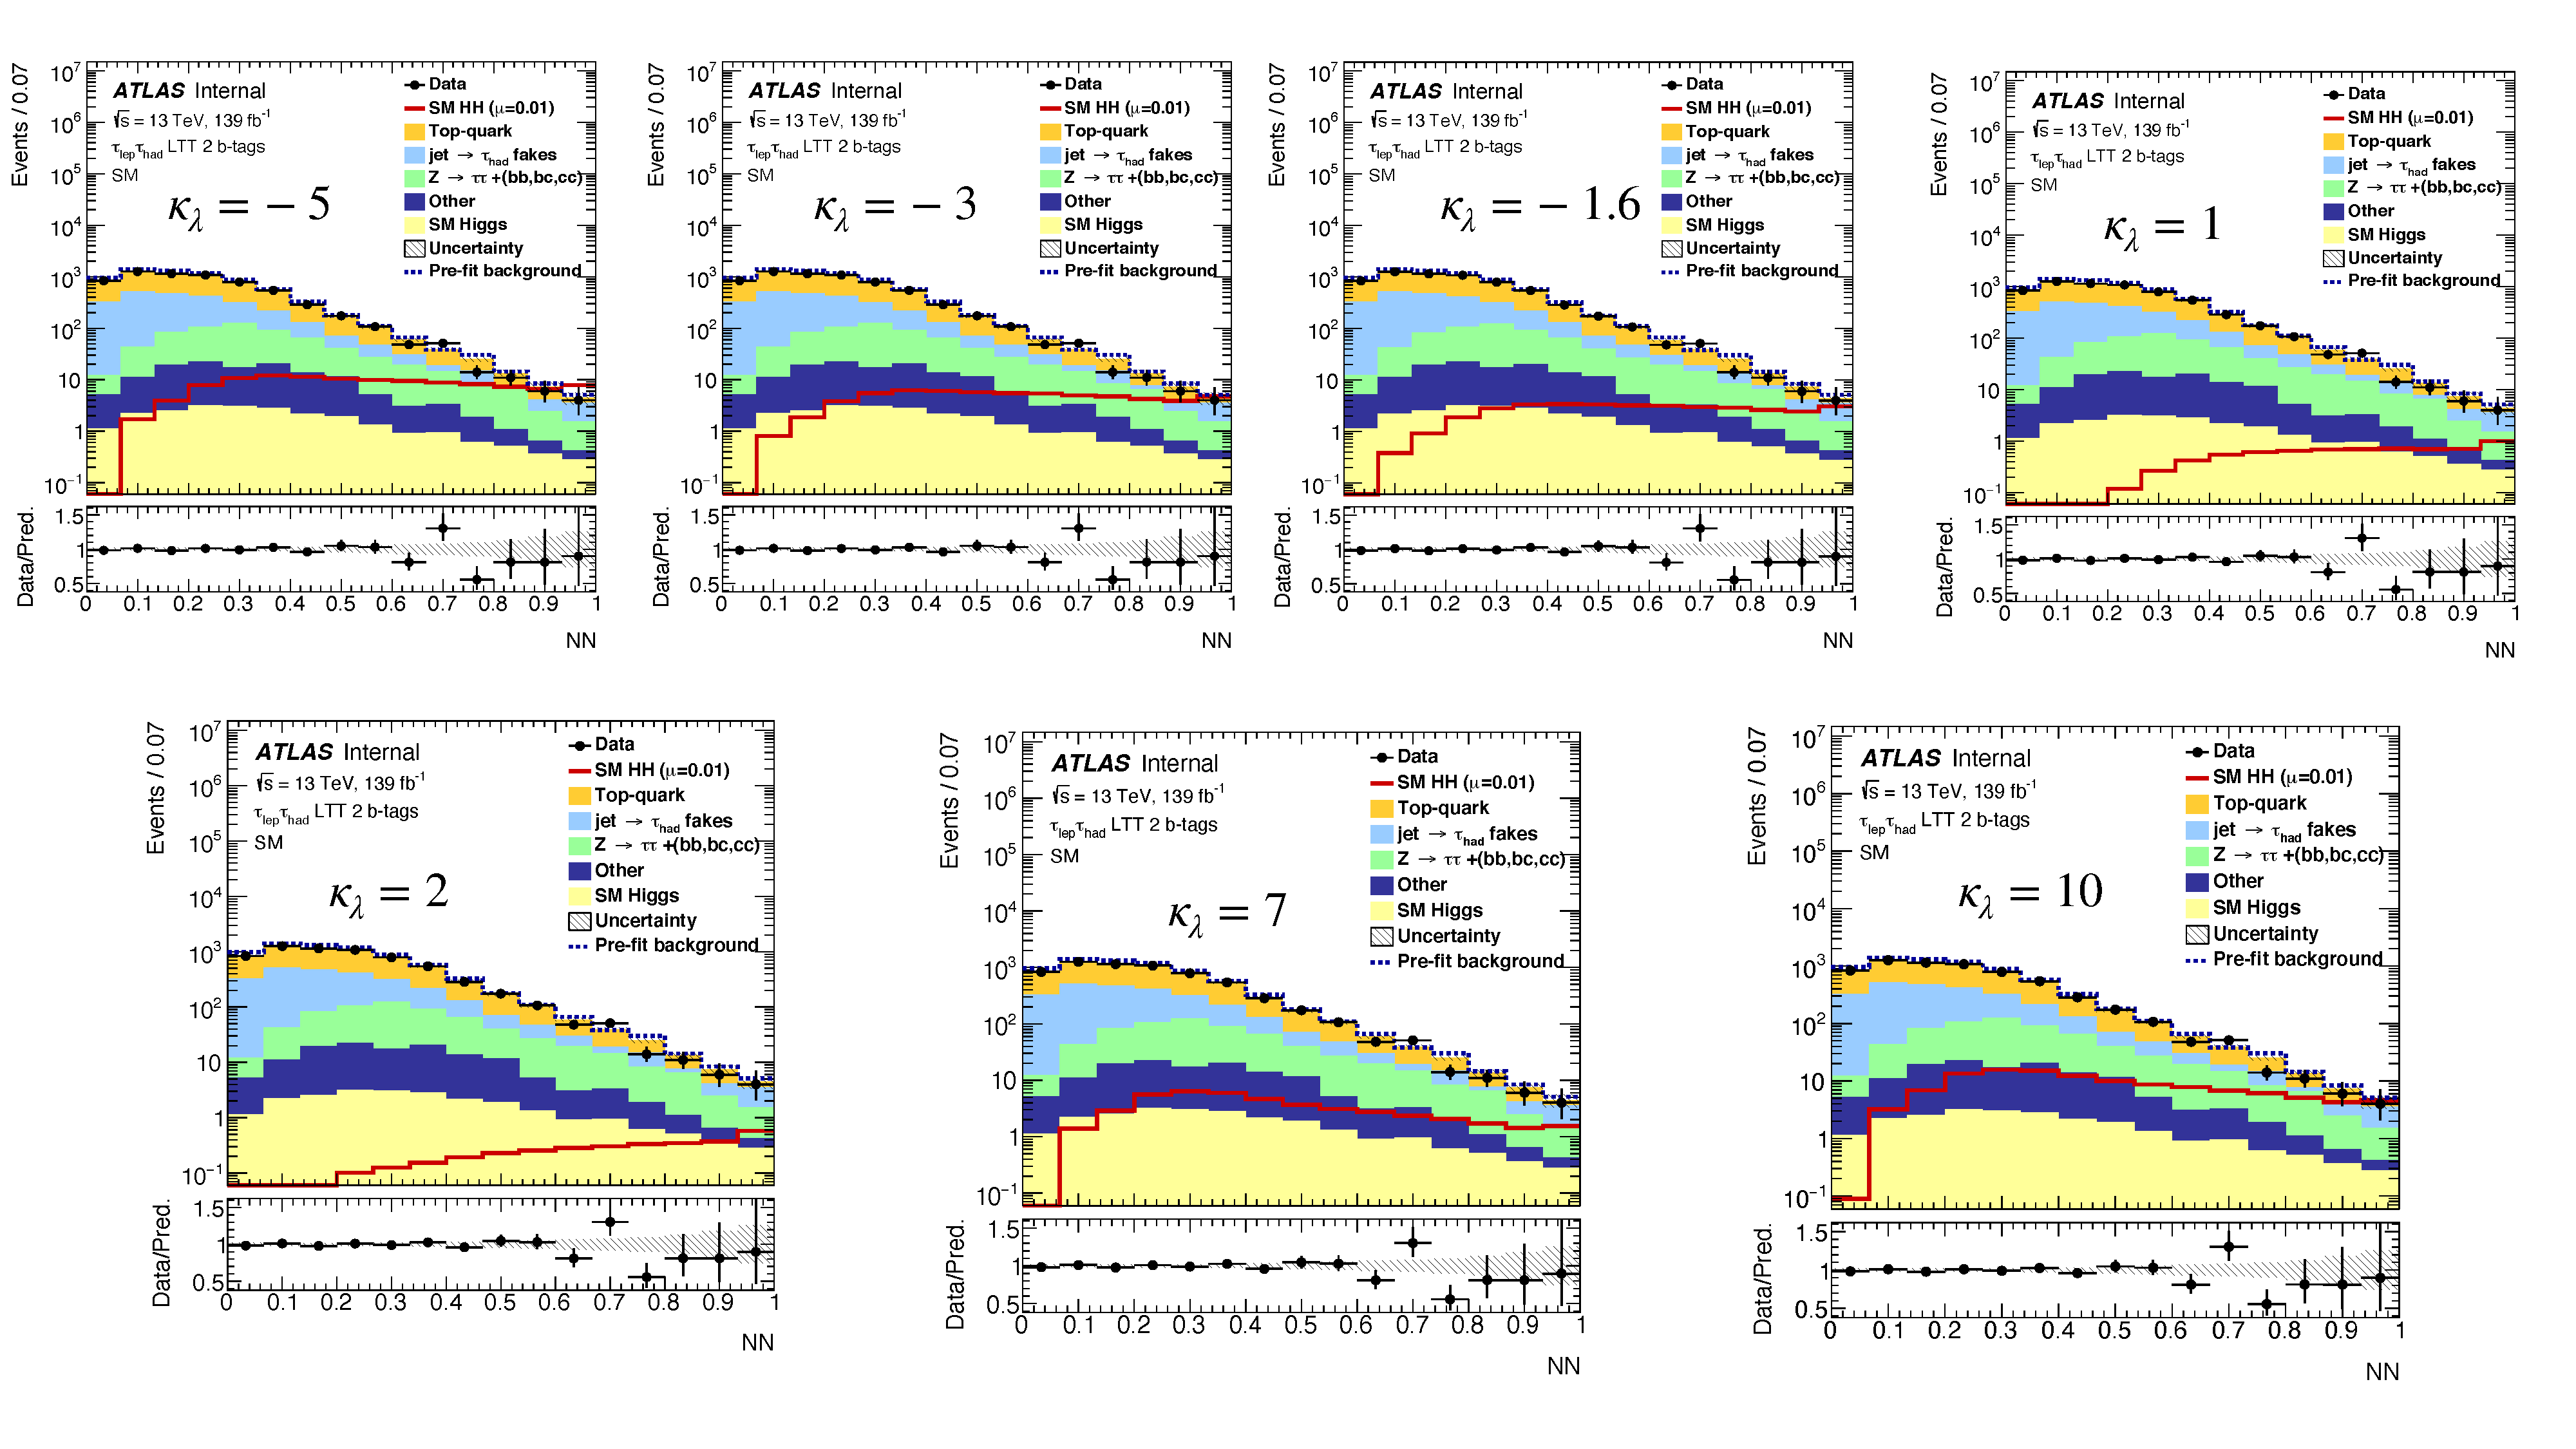
\includegraphics[width=\textwidth]{DiHiggs/plots/kl_scan/bbtautauSubchannels/bkg_only_postfit_lephad_LTT.pdf}
\end{center}
\caption{Post-fit plots of the neural network output in the $\tau_{\text{lep}}\tau_{\text{had}}$ LTT signal region, 
showing the agreement of the background-only hypthesis with the data as well as the signal prediction for different $\kappa_\lambda$ values.}
\label{fig:postfit_ltt}
\end{figure}


\newpage
\subsubsection{Limit results: \lephad only fit}


Table~\ref{sec:fit:tab:SMLepHadLimits} shows 
the limit results obtained using SLT only fit, LTT only fit, and SLT, LTT combined fit (\lephad only fit).


\begin{table}[htbp]
\centering
\begin{tabular}{|c|c|c|c|c|c|c|}
\hline
& Observed & $-2\sigma$ & $-1\sigma$ & Median & $+1\sigma$ & $+2\sigma$\\
\hline
\multicolumn{7}{|c|}{\textbf{SLT only fit}} \\
\hline
$\sigma_\text{ggF+VBF}$ [fb] & 316.93  &   132.24  &   177.54   &  246.39  &   342.90  &   459.69 \\ 
\hline
$\sigma_\text{ggF+VBF}$ StatOnly [fb] & 222.82  &   102.04  &   136.99  &  190.11  &   264.58  &   354.69 \\ 
\hline
$\mu_\text{ggF+VBF}$ & 10.91   &    4.48   &    6.01   &    8.34  &    11.60  &    15.56 \\ 
\hline
$\mu_\text{ggF+VBF}$ StatOnly & 6.80   &    3.11   &    4.18   &    5.80   &    8.07   &   10.82 \\ 
\hline
\multicolumn{7}{|c|}{\textbf{LTT only fit}} \\
\hline
$\sigma_\text{ggF+VBF}$ [fb] & 498.70  &   386.62  &   519.04  &  720.34  &  1002.50  &  1343.92 \\ 
\hline
$\sigma_\text{ggF+VBF}$ StatOnly [fb] & 322.27  &   339.61  &   455.93  &  632.75  &   880.60  &  1180.51 \\ 
\hline
$\mu_\text{ggF+VBF}$ & 16.50   &   13.08   &   17.56   &   24.36   &   33.91  &    45.46 \\ 
\hline
$\mu_\text{ggF+VBF}$ StatOnly & 9.83   &   10.36  &    13.91   &   19.31   &   26.87  &    36.02 \\ 
\hline
\multicolumn{7}{|c|}{\textbf{SLT + LTT combined fit}} \\
\hline
$\sigma_\text{ggF+VBF}$ [fb] & 267.21  &   124.49  &   167.13  &  231.94  &   322.80  &   432.73 \\ 
\hline
$\sigma_\text{ggF+VBF}$ StatOnly [fb] & 169.05  &    96.33  &   129.33  &  179.48  &   249.79  &   334.86 \\ 
\hline
$\mu_\text{ggF+VBF}$ & 9.16   &    4.22   &    5.66   &    7.86   &    10.93   &   14.66 \\ 
\hline
$\mu_\text{ggF+VBF}$ StatOnly & 5.16   &    2.94   &    3.95   &    5.48   &    7.62  &    10.22 \\ 
\hline
\end{tabular}
\caption{95\% C.L. expected and observed limit on the non-resonant HH production cross-section 
assuming SM kinematics using SLT only, LTT only and \lephad channel fit.
The signal strength is with respect to the 
SM cross-section, i.e.\ 
$\mu_\text{ggF+VBF}=\sigma_\text{ggF+VBF}/\sigma_\text{ggF+VBF}^\text{SM}$.
The `StatOnly' indicates that the limits are calculated with only statistical uncertainty,
and if not specified, the limits are obtained with full systematics.
}
\label{sec:fit:tab:SMLepHadLimits}
\end{table}
% \hline
% $\sigma_{ggF}$ [fb] & 256.29  &   119.54  &   160.48  &  222.72  &   309.96  &   415.53 \\ 
% \hline
% $\sigma_{ggF}$ StatOnly [fb] & 163.90  &    92.45  &   124.11   &   172.25  &   239.72  &   321.36 \\ 
% \hline
% $\mu_{ggF}=\sigma_{ggF}/\sigma_{ggF}^\text{SM}$ & 9.31   &    4.29   &    5.75   &    7.99  &    11.11   &   14.90 \\ 
% \hline
% $\mu_{ggF}=\sigma_{ggF}/\sigma_{ggF}^\text{SM}$ StatOnly & 5.28   &    2.98   &    4.00   &    5.55   &    7.72    &  10.35 \\ 
% \hline





Figures~\ref{fig:LepHadLimits} show the 95\% C.L. expected limits on 
the resonant HH production cross-section as a function of the resonance mass from the \hadhad and \lephad channels, respectively. 
% In the \hadhad channel an excess is observed in the resonant limits in the mass range between 900 GeV and 1100 GeV. 
% The largest local significance is at 1 TeV and it corresponds to 2.8$\sigma$ (the local significance is 2.5$\sigma$ at 900 GeV and 1.7$\sigma$ at 1.1 TeV).
No significant excess is observed in the \lephad channel (largest local significance at 1.1~TeV corresponding to 1.6~$\sigma$).

\begin{figure}[htbp]
\centering
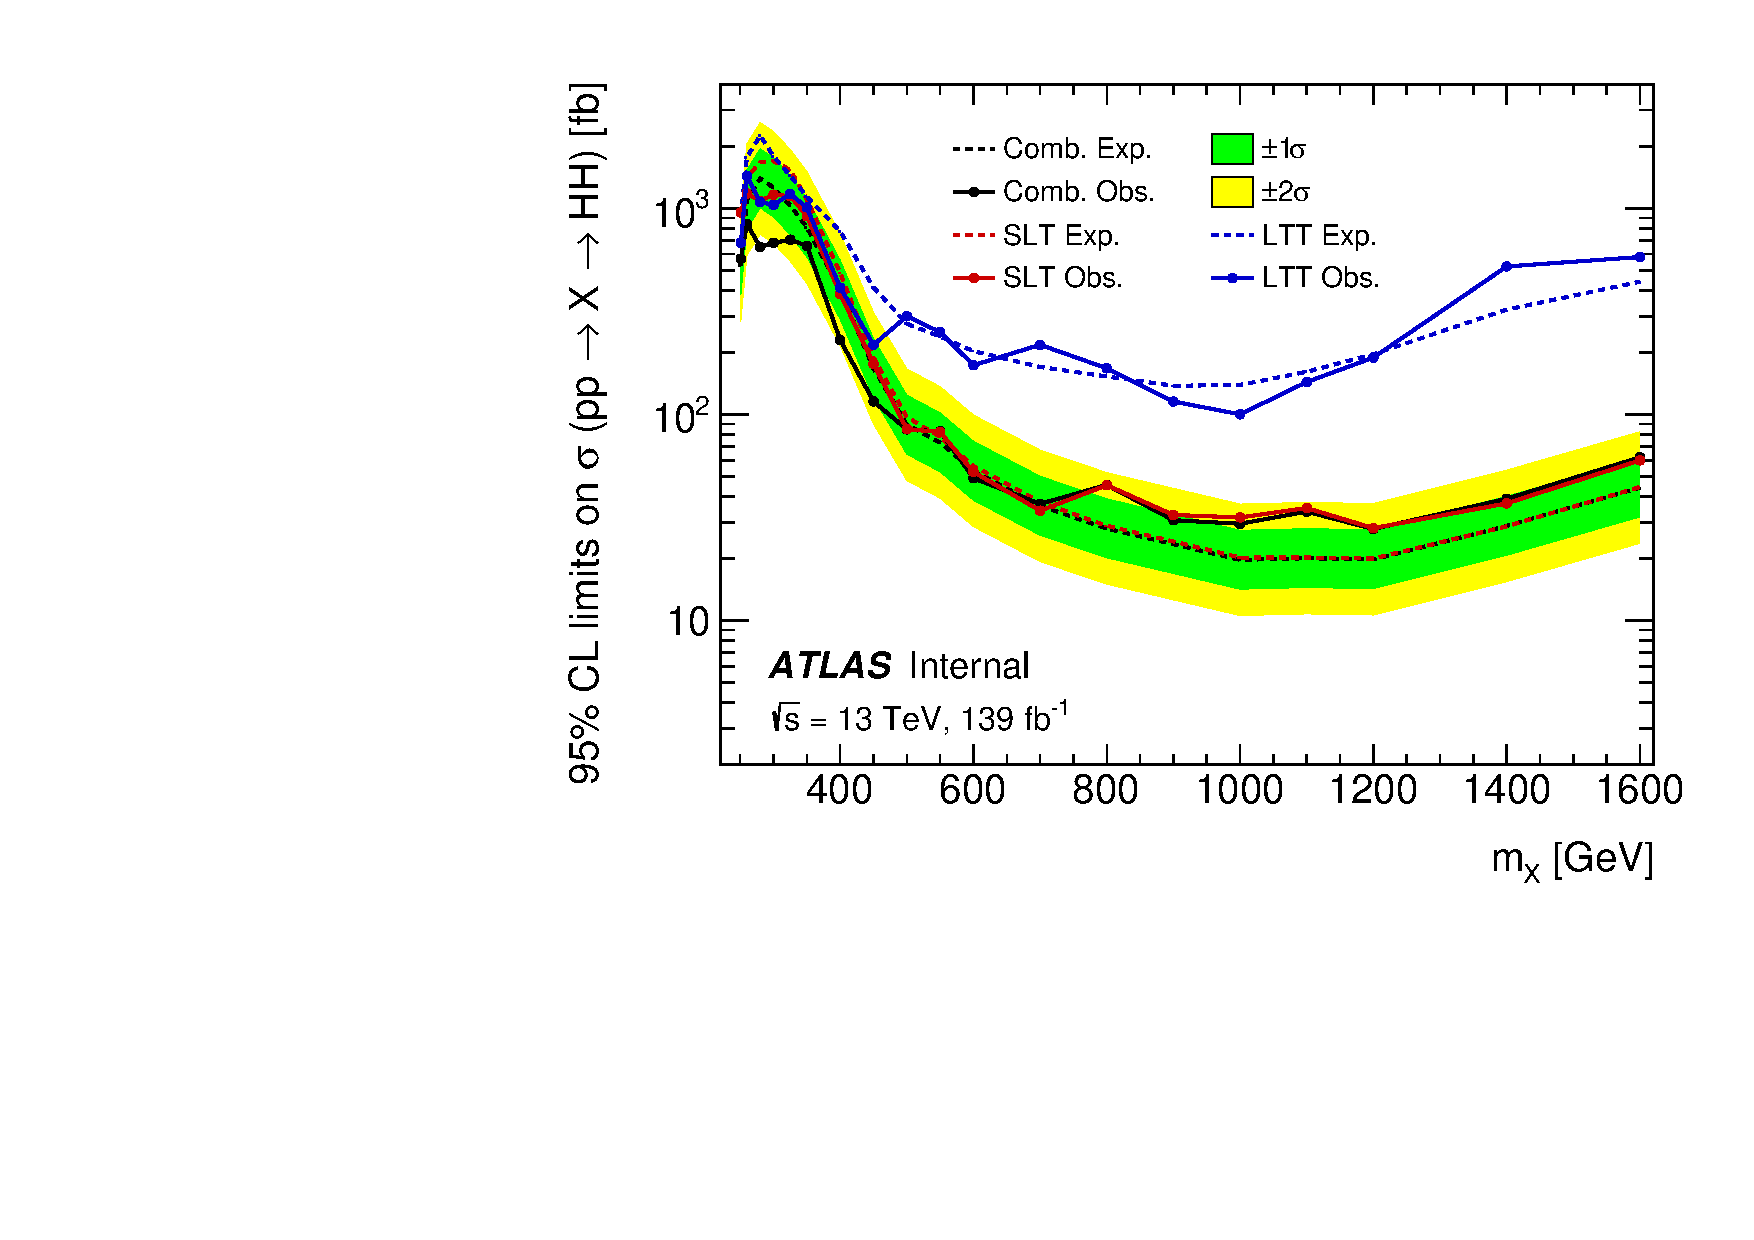
\includegraphics[width=.8\textwidth]{figures/results/HH/LepHad/LepHad_Limits_Split.pdf}
\caption{95\% C.L.\ expected and observed limits on the resonant $HH$ production cross-section
as a function of the resonance mass in the \lephad channel.
The black lines shows the \lephad channel combined limit whereas the red and blue lines 
show the limit for SLT and LTT channels separately. 
The solid and dashed lines represent the observed and expected limits respectively.}
\label{fig:LepHadLimits}
\end{figure}

% \begin{figure}[htbp]
% \centering
% 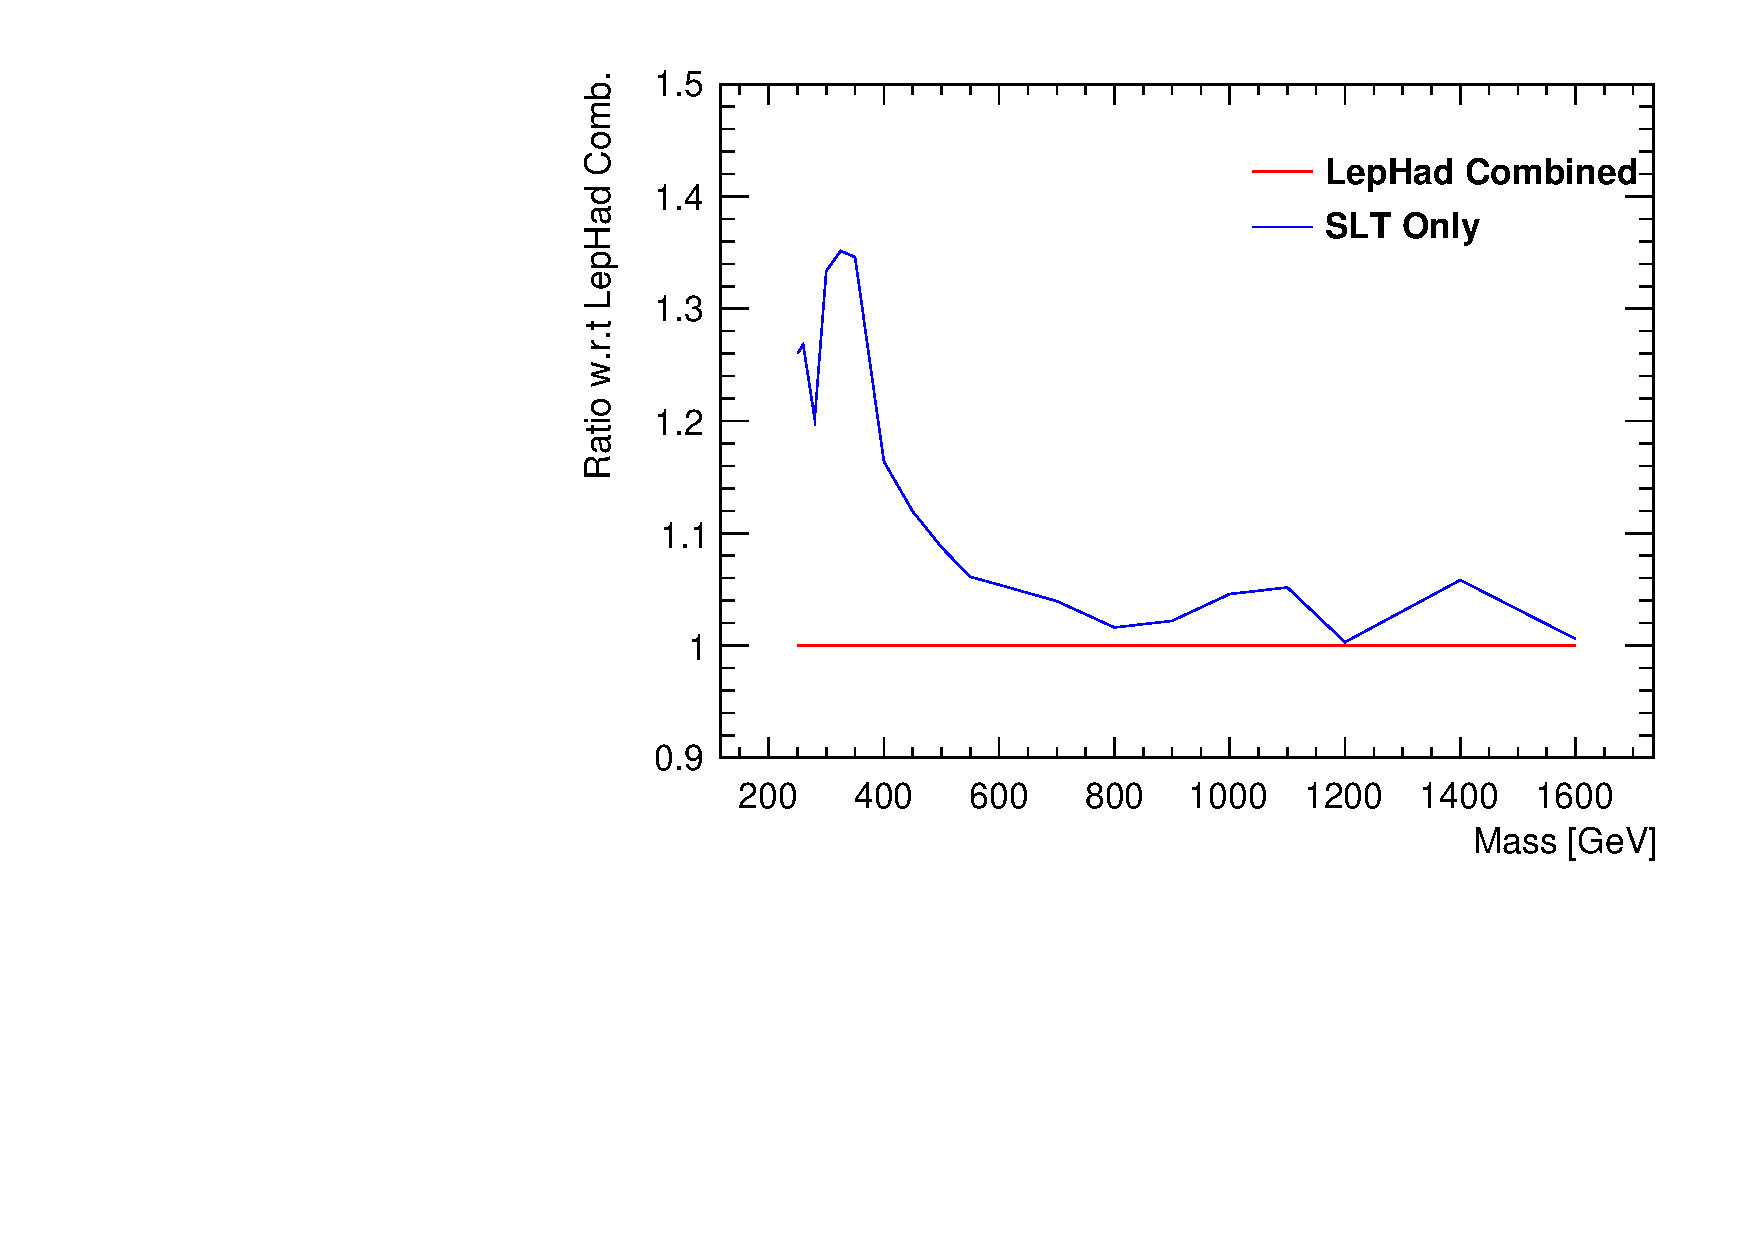
\includegraphics[width=.45\textwidth]{figures/results/HH/LepHad/SLT_LepHad.pdf}
% 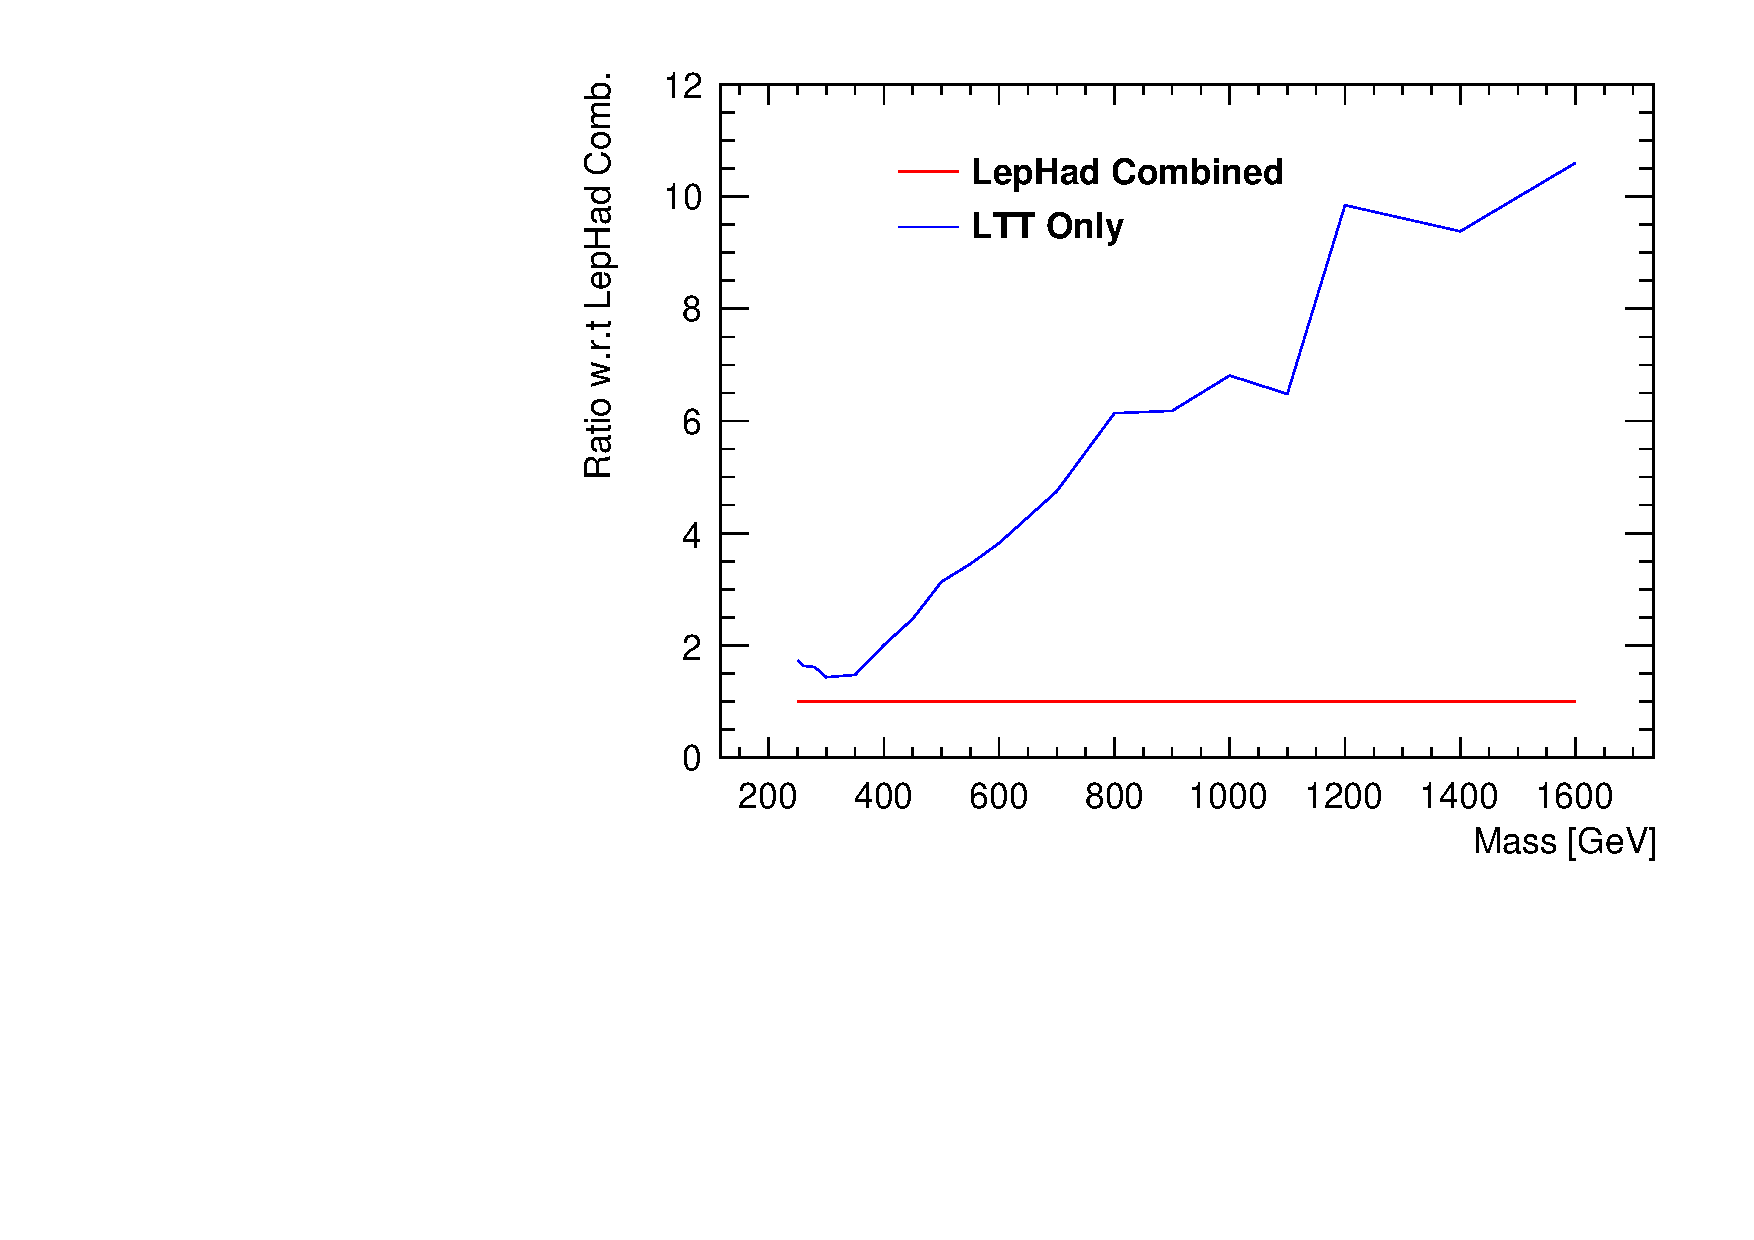
\includegraphics[width=.45\textwidth]{figures/results/HH/LepHad/LTT_LepHad.pdf}
% \caption{The ratios between SLT 95\% C.L. expected limits and \lephad combined limit (left)
% and the ratios between LTT limits and \lephad combined limit (right) as a
% function of the resonance mass.} 
% \label{fig:LepHadLimitsratio}
% \end{figure}






Upper limits at 95\% C.L.\ are set on the non-resonant $HH$ production cross-section as a function of \kl,
in the range of -10 to 10.
The \kl\ is excluded at 95\% C.L.\ outside the range of [-3.8, 12.2] ([-3.8, 11.9]) for observed (expected) limit.
The results are shown in  Figure~\ref{fig:bbtautau_subklscans}.


\begin{figure}[htbp]
\begin{center}
    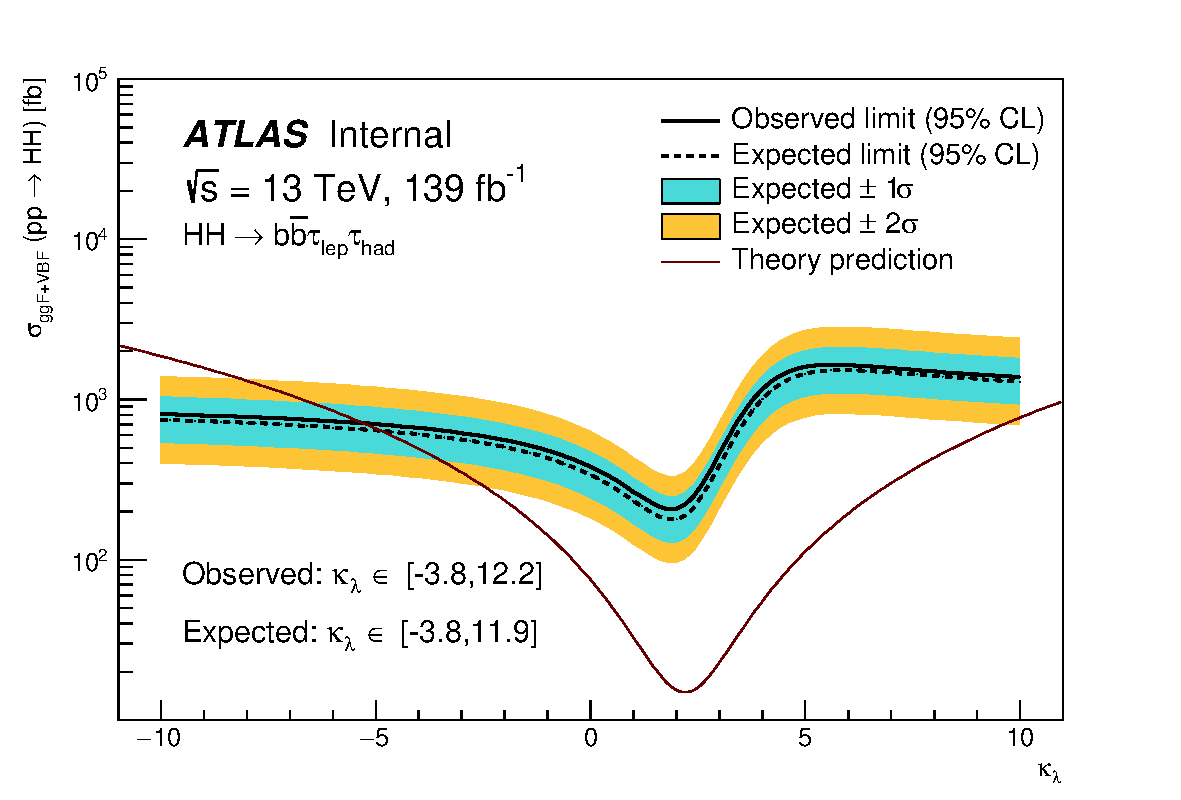
\includegraphics[width=.8\textwidth]{DiHiggs/plots/kl_scan/bbtautauSubchannels/bbtautau_lephad_kl_scan.pdf}
\end{center}
\caption{Observed and expected 95\% CL exclusion limits on non-resonant 
HH production as a function of $\kl$ in the 
using \lephad only fit.
The observed (expected) limit on $\kl$ is 
[-3.8, 12.2] ([-3.8, 11.9]).}
\label{fig:bbtautau_subklscans}
\end{figure}


\newpage

\subsection{Combination results of \lephad and \hadhad}

\label{sec:DiHiggs:combination-bbtautau}
A combined fit is then performed on all three signal regions and the \ZHF\ control region.
The combined results are shown in this section. 



Table~\ref{sec:fit:tab:SMCombinedLimits} shows 95\% C.L. expected limit on the non-resonant
HH production cross-section assuming SM kinematics from the combined fit.


\begin{table}[htbp]
\centering
\begin{tabular}{|c|c|c|c|c|c|c|}
\hline
& Observed & $-2\sigma$ & $-1\sigma$ & Median & $+1\sigma$ & $+2\sigma$\\
% \hline
% $\sigma_{ggF}$ [fb] & 130.41   &    59.05   &    79.27   &    110.02    &    153.11  &    205.25 \\
% \hline
% $\sigma_{ggF}$ StatOnly [fb] & 83.68   &    46.60  &     62.56  &     86.82   &    120.83  &    161.98 \\ 
% \hline
% $\mu_{ggF}=\sigma_{ggF}/\sigma_{ggF}^\text{SM}$ & 4.75   & 2.11   &    2.84  &     3.95  &    5.49  &    7.36 \\ 
% \hline
% $\mu_{ggF}=\sigma_{ggF}/\sigma_{ggF}^\text{SM}$ StatOnly & 2.69   & 1.50   &    2.01   &    2.80   &    3.89  &    5.22 \\ 
% \hline
\hline
$\sigma_\text{ggF+VBF}$ [fb] & 135.27   & 61.35  &   82.36  &   114.31   &   159.08  &   213.26 \\ 
\hline
$\sigma_\text{ggF+VBF}$ StatOnly [fb] & 85.58  &    48.45  &   65.04  &  90.27  &   125.63  &   168.41 \\ 
\hline
$\mu_\text{ggF+VBF}$ & 4.65  &     2.08   &    2.79   &    3.87  &    5.39  &    7.22 \\ 
\hline
$\mu_\text{ggF+VBF}$ StatOnly & 2.61   &    1.48   &    1.98   &    2.75   &    3.83  &    5.14 \\ 
\hline
\end{tabular}
\caption{95\% C.L. expected and observed limit on the non-resonant HH production cross-section 
assuming SM kinematics using \lephad and \hadhad combined fit.
The signal strength is with respect to the 
SM cross-section, i.e.\ 
$\mu_\text{ggF+VBF}=\sigma_\text{ggF+VBF}/\sigma_\text{ggF+VBF}^\text{SM}$.
The `StatOnly' indicates the limits are calculated with only statistical uncertainty,
and if not specified, the limits are obtained with full systematics.}
\label{sec:fit:tab:SMCombinedLimits}
\end{table}

The 95\% C.L. expected and the observed limits on the 
resonant $HH$ production cross-section, as a function of the resonance mass from the 
\lephad and \hadhad combined fit are shown in Figure~\ref{fig:CombinedLimits}.
Observed (expected) upper limits range from 26 -- 950 fb (12 -- 850 fb), 
depending on the mass of the resonance.
In the combined fit, excess (observed limit deviates greater than 2~$\sigma$ from the expected limit)
is present in the mass range between 800 and 1100~GeV. 
The maximum excess is found at the 1000~GeV which has a deviation of
of 3.1~$\sigma$. 
The local p-values as a function of resonance mass are shown in Figure~\ref{fig:CombinedPValues}.
The look-elsewhere effect is accounted by calculating the global significance
following Ref.\cite{global-significance}, using the up-crossing method:
\[ p_\text{global} = p_\text{local} +  N_\text{up} e^{-1/2(Z^2_\text{local} - Z^2_\text{ref})},
\]
where the $p_\text{local}$ and $p_\text{global}$ are the local and global p-values, and
$Z_\text{ref}$ is chosen for p=0.5 (corresponding to 0~$\sigma$ significance level), 
and $N_\text{up}$ is the number of times the local p-value curve crossing the reference line (in this case,
p=0.5) in the upwawrd direction.
The estimated global significance is $2.1^{+0.4}_{-0.2} \sigma$.


\begin{figure}[htbp]
\centering
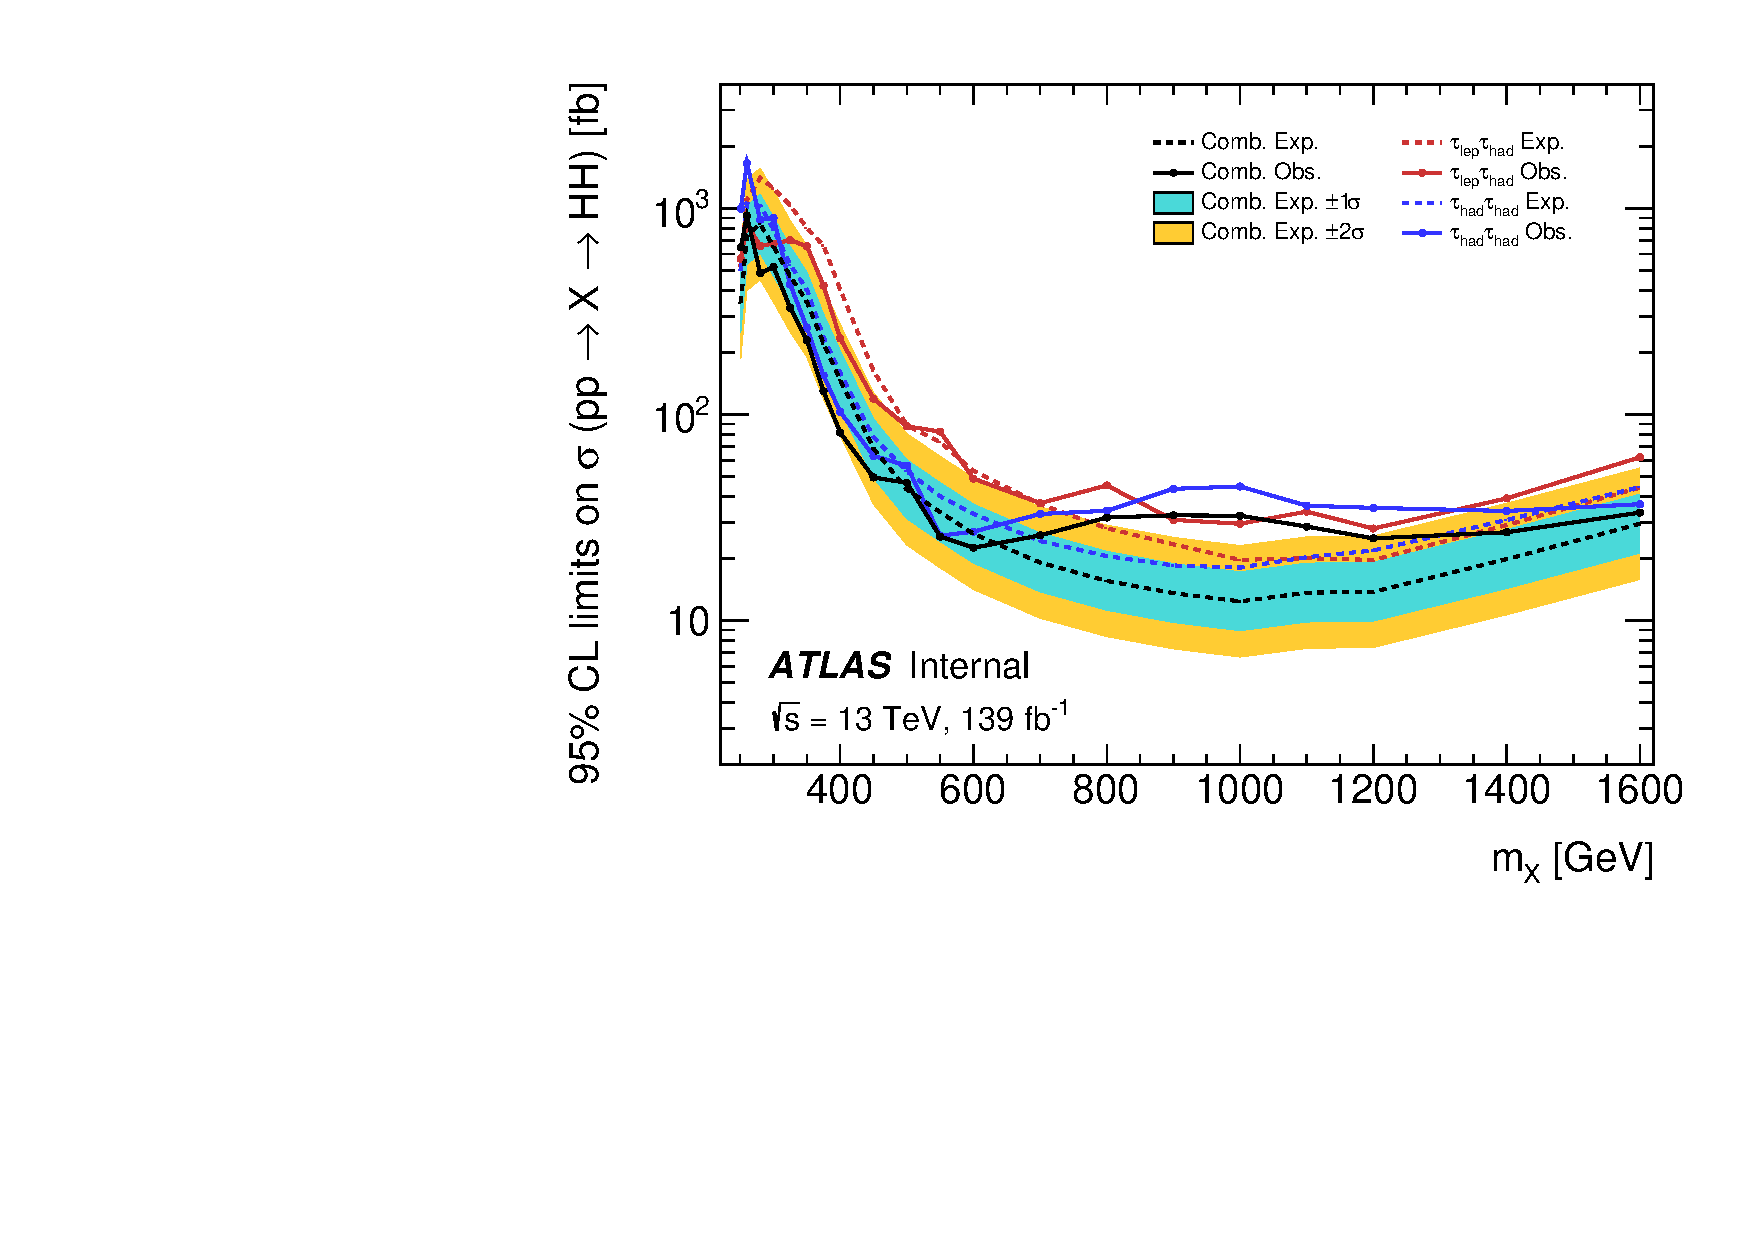
\includegraphics[width=.8\textwidth]{figures/results/HH/Combined/CombSysts_21072021.pdf}
\caption{95\% C.L. expected and observed limits on the resonant HH production cross-section as a function of the resonance mass. 
The dashed lines show the expected limits, while the solid lines show the observed limits. 
Black, red and blue represents the upper limit from combination, \lephad channel and \hadhad channel, respectively.}
\label{fig:CombinedLimits}
\end{figure}


\begin{figure}
\centering
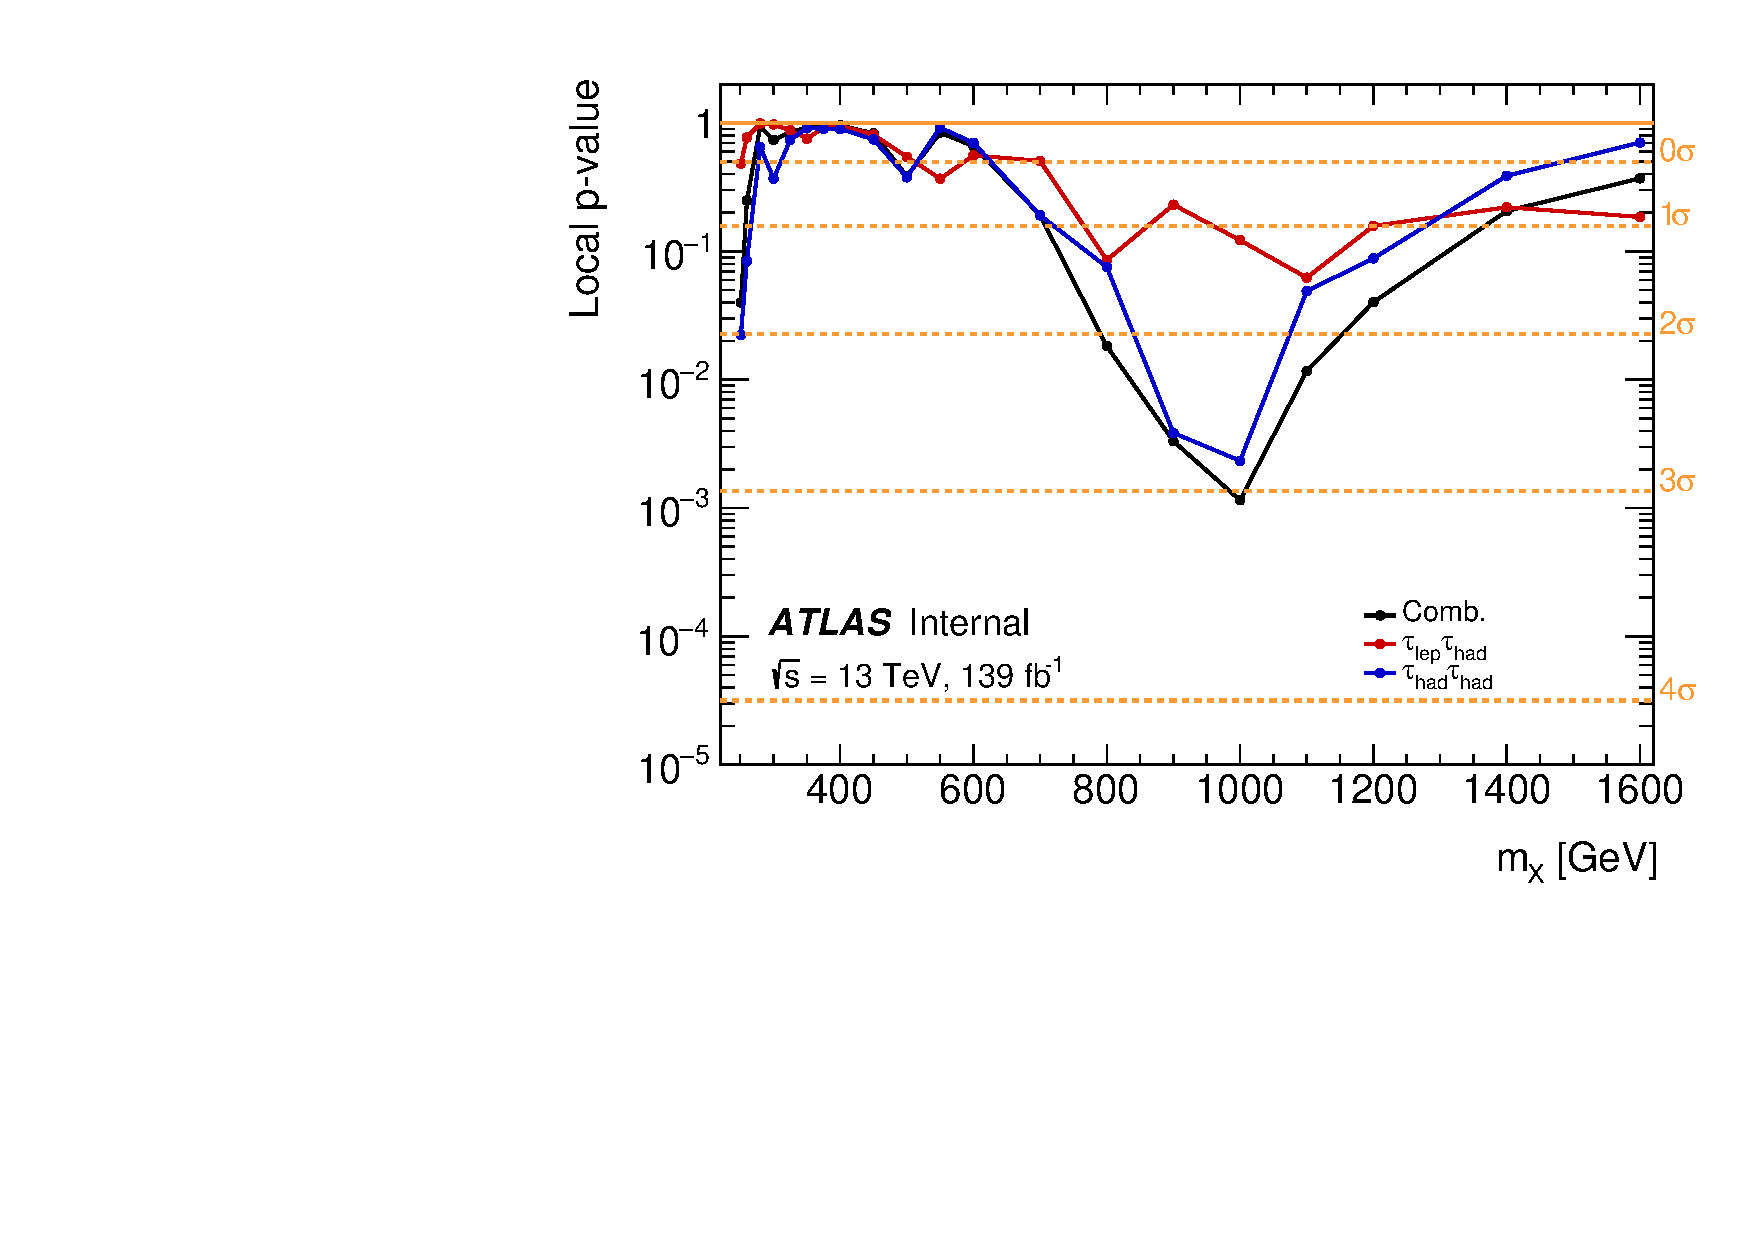
\includegraphics[width=.8\textwidth]{figures/results/HH/Combined/CombObsPvalues_21072021.pdf}
\caption{Local p-value of the background only hypothesis test as a function of the mass of the resonance. 
The black line represents the p-value from combination, while red and blue line are those 
for the \lephad and \hadhad channel, respectively. 
The horizontal dashed orange lines show the corresponding (2-side) significance level.}
\label{fig:CombinedPValues}
\end{figure}

The 95\% C.L.\ expected and the observed upper limits on the cross-section of non-resonant $HH$ production 
as a function of $\kappa_\lambda$ are shown in Figure~\ref{fig:kl_scan_individual_channels}.
The 95\% C.L.\ observed (expected) exclusion limit of $\kappa_\lambda$ is $-2.4 < \kappa_\lambda < 9.2$ 
($-2.0< \kappa_\lambda < 9.0$).

\begin{figure}[htbp]
\centering
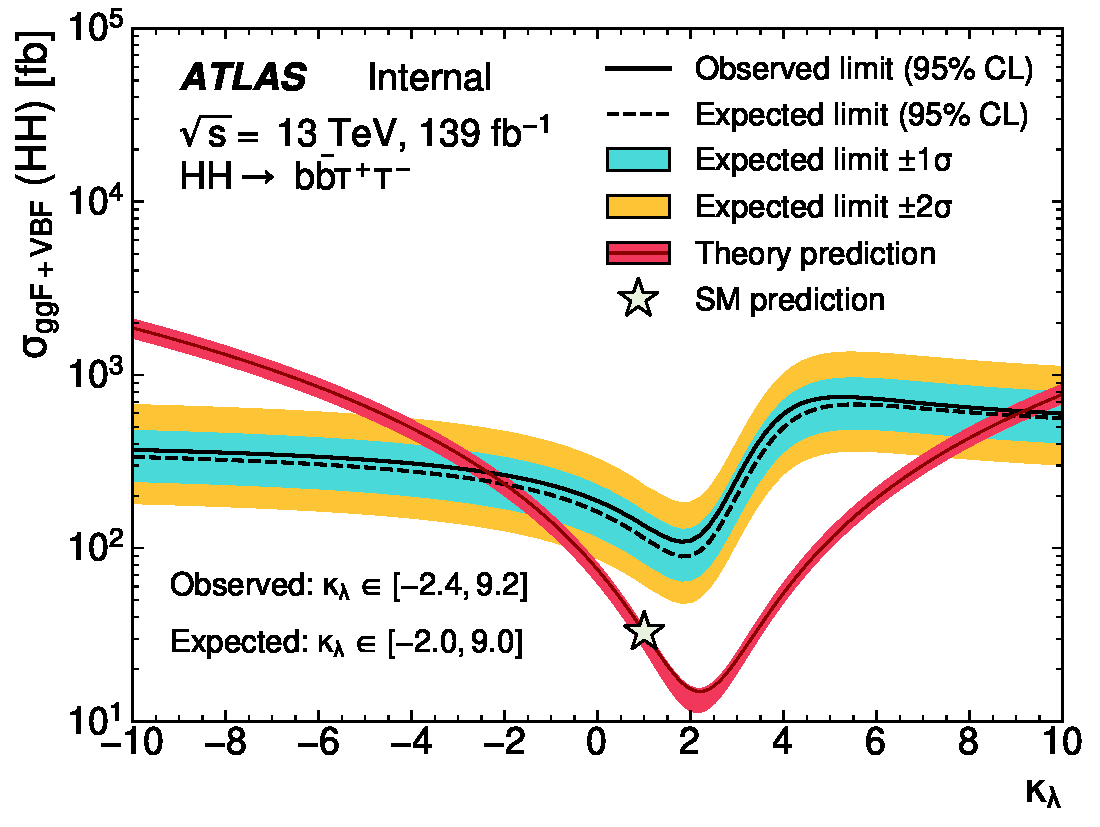
\includegraphics[width=0.8\textwidth]{DiHiggs/plots/kl_scan/20210926/bbtautau_kl_scan_mH125.pdf}
\caption{Observed and expected 95\% CL upper limits on non-resonant $\sigma(pp \rightarrow HH)$ 
    cross-section  as a function of $\kappa_\lambda$ using \lephad and \hadhad combined fit.
    The observed (expected) exclusion limit at 95\% C.L. on $\kappa_\lambda$ in the \bbtautau channel is: 
    [-2.4, 9.2] ([-2.0, 9.0]). 
}
\label{fig:kl_scan_individual_channels}
\end{figure}



\newpage

\subsection{Combination results with other $HH$ decay channels}
\label{sec:DiHiggs:combination-HH}
To maximise the sensitivity in the $HH$ searches, 
the \bbtt results are combined with other $HH$ decay channels results.
The \bbtt non-resonant $HH$ result is combined to the \bbyy channel, 
which also has high sensitivity due to the high energy resolution in 
di-photon systems.
For the resonant searches, the \bbtt results are combined with
\bbyy and \bbbb channels.
The \bbyy channel is expected to have high sensitivity in low energy
regime and the \bbbb channel dominates over the high-energy regime, which
benefits from high selection efficiency in the more boosted events topology.



\subsubsection{Combination results of \bbtt and \bbyy}

The \bbtt results are combined with the results in \bbyy channel 
in terms of upper limits on the non-resonant $HH$ production signal strength $\mu$, 
and on cross-section as a function of \kl~\cite{ATLAS-CONF-2021-052}.
The upper limits on signal strength 
are shown in Table~\ref{tab:results_nonres_exp_limits}, and the
limits on the cross-section are shown in Figure~\ref{fig:kl_scan_combined}.
This combination result sets the current world-best observed upper limit on the SM $HH$ cross-section
~\cite{PhysRevLett.122.121803,  CMS-PAS-HIG-20-004, CMS-PAS-HIG-20-005,CMS-HIG-19-018}, 3.1 times 
SM cross-section, at 95\% C.L. 

\begin{table}[htbp]
\sisetup{}
\begin{center}

\begin{tabular}{l
S[round-mode=places, round-precision=1]|
S[round-mode=places, round-precision=1]
S[round-mode=places, round-precision=1]
S[round-mode=places, round-precision=1]
S[round-mode=places, round-precision=1]
S[round-mode=places, round-precision=1]
}
\toprule
& {Obs.} & $\SI{-2}{\sigma}$ & $\SI{-1}{\sigma}$ & {Exp.} & $\SI{+1}{\sigma}$ & $\SI{+2}{\sigma}$ \\
\midrule
% {cross-section} & & & & & & & \\
% % \bbbb & $-$ & $4.806748$ & $6.453069$ & $8.955687$ & $12.514435$ & $16.953666$ \\
% \bbtautau &    4.126402 &           1.871041 &           2.511876 &    3.486028 &           4.973379 &           7.015396 &  2.995979 &  2.312411 & \\
% \bbyy &    4.058352 &           2.905606 &           3.900781 &    5.413576 &           7.998831 &          11.986507 &  5.327046 &  3.790706 &  \\
% Combined &    2.786297 &           1.510250 &           2.027514 &    2.813821 &           4.002772 &           5.619012 &  2.486833 &  1.682553 &  \\
% \midrule
%{Signal strength} & & & & & & & \\
\bbyy &         4.308676 &           3.083336 &           4.139384 &    5.744714 &           8.821852 &          14.253823  \\
\bbtautau &    4.644017 &           2.072931 &           2.782913 &    3.862179 &           5.871155 &           9.380173   \\
\midrule
Combined &    3.056996 &           1.657194 &           2.224786 &    3.087599 &           4.657015 &           7.342502   \\

\bottomrule
\end{tabular}
\caption{Observed and expected $\SI{95}{\percent}$ C.L.\ upper limits on the 
signal strength for SM \HH production derived from the \bbtt and \bbyy searches,
and their statistical combination. 
}
\label{tab:results_nonres_exp_limits}
\end{center}

\end{table}



\begin{figure}[htbp]
\centering
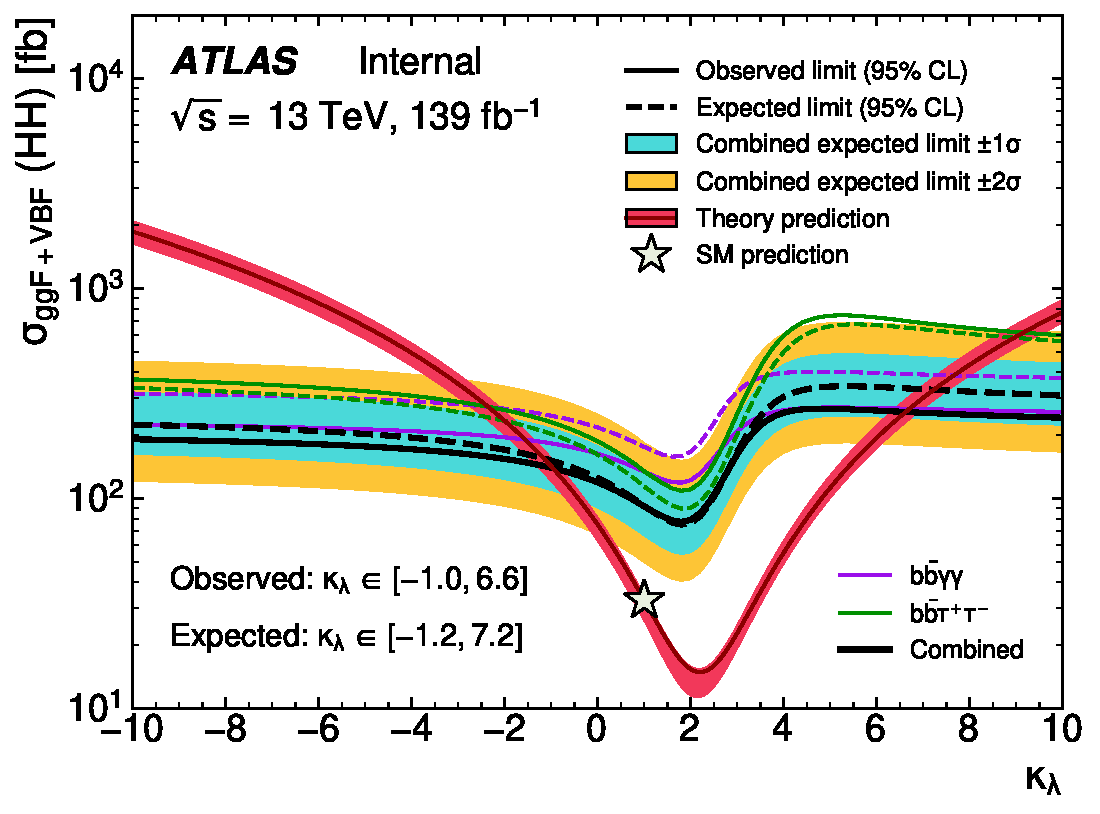
\includegraphics[width=0.8\textwidth]{DiHiggs/plots/kl_scan/20210926/all_channels_kl_scan_mH125.pdf}
\caption{Observed and expected 95\% CL exclusion limits on non-resonant $\sigma(pp \rightarrow HH)$ as a function of $\kappa_\lambda$ for the individual channels and the combination of \bbtt and \bbyy.
The observed (expected) combined limit on $\kappa_\lambda$ is:  [-1.0, 6.6]  ([-1.2 , 7.2]).
}
\label{fig:kl_scan_combined}
\end{figure}



\subsubsection{Combination results of \bbtt, \bbyy and \bbbb}

% The resonant $HH$ searches target a heavy, spin-0 scalar $X$, 
% which has a narrow-width compared to the experimental mass resolution. 
Observed and expected limits at 95\% C.L.\  are set on the resonant $HH$ production cross-section, 
$\sigma(X \rightarrow HH$, for \bbyy, \bbtt, and \bbbb searches, and their statistical combination~\cite{ATLAS-CONF-2021-052},
as shown in 
Figure~\ref{fig:spin0_obs_limits}.
The observed (expected) combined limits on cross-section range from 1.1 to 595~fb (1.2 to 392~fb) depending 
on the resonance mass.
As mentioned before, the \bbyy results shows largest sensitive low \mX, and the \bbbb limits dominates in high \mX.
The \bbtt search is the most sensitive in the intermediate range, around 400--800~GeV.
These three channels are therefore complementary to each other. 

The largest excess is observed at \SI{1.1}{\tev}, corresponding to a local significance of
3.2~$\sigma$. While the similar excess is observed in the \bbtt channel, the compatibility 
is checked with the \bbbb excess. At 1.1 \tev, the level of compatibility
of the fitted signal strength in the two channels corresponds to a p-value
of 0.34 ($>>$0.05), and hence the excess is compatible.


% The global significance is estimated to be 2.1~$\sigma$
% This feature has been investigated, and the local (global) significance for $\mX = \SI{1.1}{\tev}$ 
% using the asymptotic formula is found to be 3.2~$\sigma$ (2.1~$\sigma$).
%~\cite{Gross_2010}

\begin{figure}[htbp]
\centering
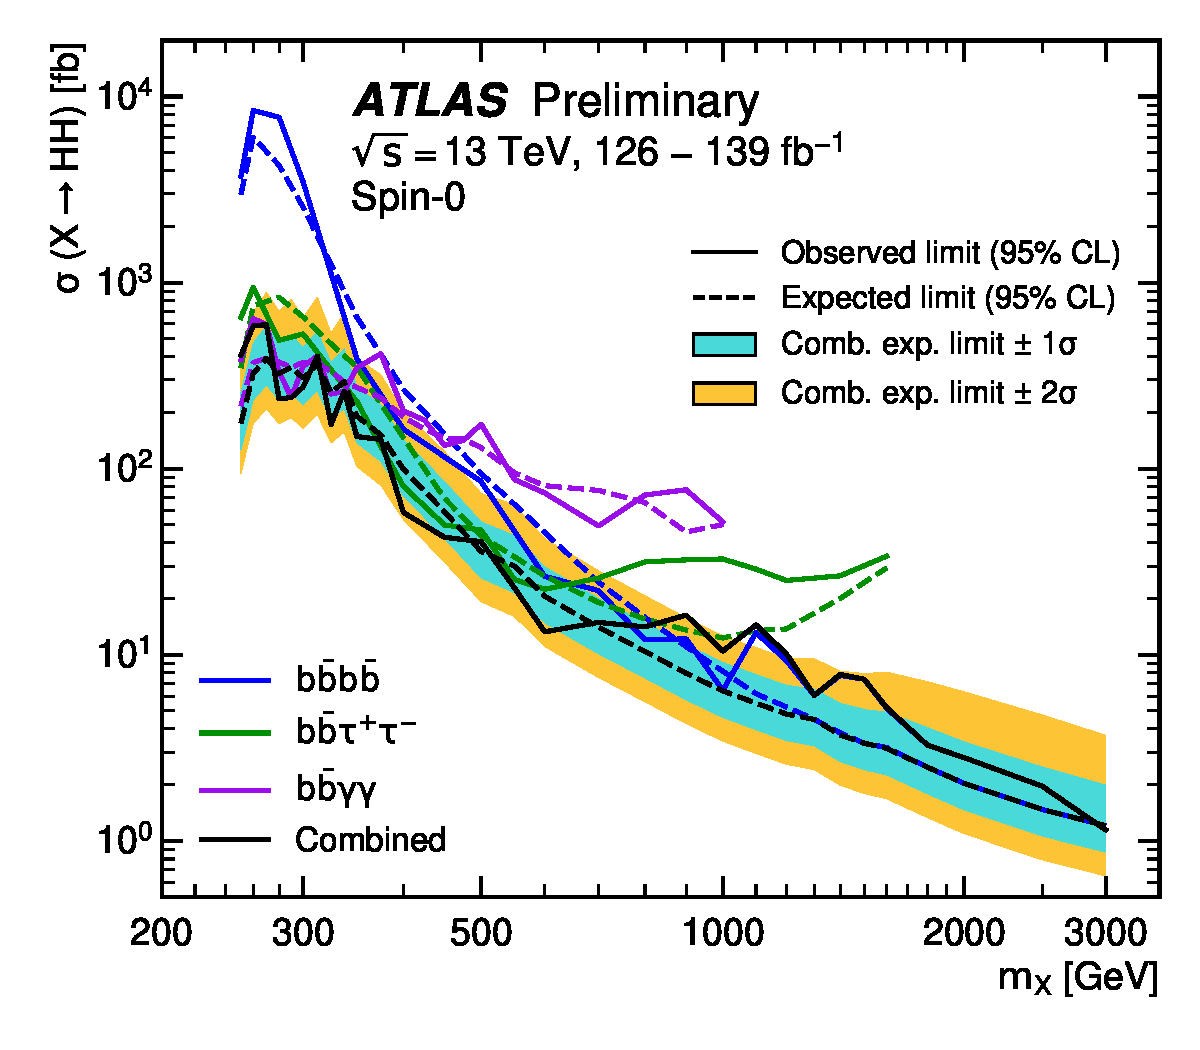
\includegraphics[height=0.45\textheight]{DiHiggs/plots/upperlimit_xsec_spin0_json_obs_fullcorr.pdf}
%\subfloat[Local $p$-value]{\includegraphics[width=0.5\textwidth]{figures/pvalue/\pvaluedate/spin0/spin0_local_pvalue.pdf}}
\caption{Expected and observed 95\% C.L.\ upper limits on $\sigma(X \rightarrow HH$ 
for a spin-0 resonance as a function of its mass \mX in the \bbyy, \bbtt and \bbbb searches, 
and their statistical combination. 
% The discontinuities in the limit visible in the range
%  $\mX < \SI{400}{\gev}$ are caused by the partial availability of the different analysis limits on 
%  a point-by-point basis, which are provided only for the \bbyy search at the weakest limit points. 
%  Further details can be found in \Tabrange{\ref{tab:spin-0-individual-fullcorr-1}}{\ref{tab:spin-0-individual-fullcorr-4}} in the appendix.
}
\label{fig:spin0_obs_limits}
\end{figure}
